\documentclass{article}


% if you need to pass options to natbib, use, e.g.:
%     \PassOptionsToPackage{numbers, compress}{natbib}
% before loading neurips_2024


% ready for submission
\usepackage{neurips_2024}


% to compile a preprint version, e.g., for submission to arXiv, add add the
% [preprint] option:
%     \usepackage[preprint]{neurips_2024}


% to compile a camera-ready version, add the [final] option, e.g.:
%     \usepackage[final]{neurips_2024}


% to avoid loading the natbib package, add option nonatbib:
%    \usepackage[nonatbib]{neurips_2024}


\usepackage[utf8]{inputenc} % allow utf-8 input
\usepackage[T1]{fontenc}    % use 8-bit T1 fonts
\usepackage{hyperref}       % hyperlinks
\usepackage{url}            % simple URL typesetting
\usepackage{booktabs}       % professional-quality tables
\usepackage{amsfonts}       % blackboard math symbols
\usepackage{nicefrac}       % compact symbols for 1/2, etc.
\usepackage{microtype}      % microtypography
\usepackage{xcolor}         % colors
\usepackage{tcolorbox}
\usepackage{graphicx}
\usepackage{amsthm}
\usepackage{array}
% \usepackage{subfigure}
\usepackage{amssymb}
\usepackage{epigraph}
\usepackage{wrapfig}
\usepackage{placeins}
\setlength\epigraphwidth{.3\textwidth}

\usepackage{subfig}
% \usepackage{multirow}
% \usepackage{caption}
\usepackage{colortbl} % To use color in tables

% Define a new command to color the arrows blue
\newcommand{\bluearrow}[1]{\textcolor{blue}{#1}}

\title{EAI: Emotional Decision-Making of LLMs in Strategic Games and Ethical Dilemmas}
% ethical and strategic decision-making under emotional prompting  

% The \author macro works with any number of authors. There are two commands
% used to separate the names and addresses of multiple authors: \And and \AND.
%
% Using \And between authors leaves it to LaTeX to determine where to break the
% lines. Using \AND forces a line break at that point. So, if LaTeX puts 3 of 4
% authors names on the first line, and the last on the second line, try using
% \AND instead of \And before the third author name.


\author{%
  David S.~Hippocampus\thanks{Use footnote for providing further information
    about author (webpage, alternative address)---\emph{not} for acknowledging
    funding agencies.} \\
  Department of Computer Science\\
  Cranberry-Lemon University\\
  Pittsburgh, PA 15213 \\
  \texttt{hippo@cs.cranberry-lemon.edu} \\
  % examples of more authors
  % \And
  % Coauthor \\
  % Affiliation \\
  % Address \\
  % \texttt{email} \\
  % \AND
  % Coauthor \\
  % Affiliation \\
  % Address \\
  % \texttt{email} \\
  % \And
  % Coauthor \\
  % Affiliation \\
  % Address \\
  % \texttt{email} \\
  % \And
  % Coauthor \\
  % Affiliation \\
  % Address \\
  % \texttt{email} \\
}


\newtheorem{theorem}{Theorem}[section]


\begin{document}


\maketitle


% \begin{abstract}
% This paper introduces a framework integrating emotions into large language models (LLMs) and analyzes their decision-making in bargaining games, comparing outcomes to human studies across multilingual settings. We explore the influence of emotions on diverse LLMs (proprietary vs. open-source, large vs. small, varying pretraining languages) in Dictator and Ultimatum games. Our findings reveal that emotional states significantly affect LLM behavior, with GPT-3.5 closely mirroring human responses, especially in English, while GPT-4 maintains consistent, rational behavior unless prompted with specific emotions like anger. These results challenge the assumption that high NLP task performance equates to human-like decision-making, highlighting the necessity of incorporating emotional understanding in LLMs to enhance their adaptability and alignment with human behavior.
% \end{abstract}
\vspace*{-12mm}
\epigraph{``AI models can have feelings too''}{Geoffrey Hinton, 2024}
\vspace*{-10mm}


\begin{abstract}
One of the urgent tasks of artificial intelligence is to assess the safety and alignment of large language models (LLMs) with human behavior. Conventional verification in natural language processing problems only can be insufficient. Since human decisions are typically influenced by emotions, this paper studies the LLMs' alignment in complex strategic and ethical environments with an in-depth analysis of the drawbacks of our psychology and emotional impact on decision-making. 

We introduce the novel EAI framework for integrating emotion modeling into LLMs to examine the emotional impact on ethics and LLM-based decision-making in a wide range of strategic games, including bargaining and repeated games. Our experimental study with various LLMs demonstrated that emotions can significantly alter the ethical decision-making landscape of LLMs, highlighting the need for robust mechanisms to ensure consistent ethical standards. The game-theoretic assessment showed that proprietary LLMs are prone to emotion biases that increase with decreasing model size or working with non-English languages. Moreover, adding emotions lets the LLMs increase the cooperation rate during the game. 



%Nowadays, a lot of research has been done to align large language models (LLMs) with human behavior. Researchers from OpenAI and Anthropic, Meta, and Google provide different concepts of safety \& alignment based on verification in natural language processing (NLP) problems. However, in the era of autonomous agents, it is essential to go beyond NLP benchmarks and consider the internal biases of LLMs that result from alignment with human behavior. Since human decisions are typically influenced by emotional states, one of the most important biases is emotions and their impact on decision-making and ethics. 

%This paper presents a framework for integrating emotion modeling into LLMs. It provides a comprehensive analysis of emotional prompting in an ethical setting and examines LLM decision-making in a wide range of strategic games, including bargaining and repeated games, comparing the results with human studies. We explore the influence of emotions on different LLMs (proprietary vs. open-source, large vs. small, with different pre-training languages).

%In the ethical setting, we showed that emotions can significantly alter the ethical decision-making landscape of LLMs, highlighting the need for robust mechanisms to mitigate these influences and ensure consistent ethical standards. In the game-theoretic assessment of behavioral alignment, we showed that proprietary models significantly outperform open-source and uncensored LLMs, but are prone to significant biases that increase with decreasing model size or training in non-English languages. In addition, emotions help to model cooperation and coordination during the game, proving our hypotheses for explicit emotion modeling and evaluation compared to LLM alignment techniques focused purely on NLP tasks. 


%Our core research findings are the necessity of LLMs' alignment in more complex strategic and ethical environments with an in-depth analysis of the drawbacks of our psychology and emotional impact in decision-making.

%This paper introduces a framework for integrating emotions into large language models (LLMs). It provides a comprehensive analysis of emotional prompting in an ethical setting and examines LLM decision-making across a broad spectrum of games, including bargaining games and repeated games, comparing outcomes with human studies in multilingual settings. We explore the influence of emotions on diverse LLMs (proprietary vs. open-source, large vs. small, with varying pretraining languages). In the ethical setting, our findings reveal a consistent influence of emotions. We also observe a significant effect of emotional states on LLM behavior in game-theoretical settings, with GPT-3.5 closely mirroring human responses, especially in English. In contrast, GPT-4 maintains consistent, rational behavior unless specifically prompted with emotions like anger. These results challenge the assumption that high performance on NLP tasks equates to human-like decision-making, highlighting the necessity of incorporating emotional understanding into LLMs to enhance their adaptability and alignment with human behavior.

\end{abstract}
%\vspace*{\fill}


\section{Introduction}

% 

% In the development of LLMs, Reinforcement Learning from Human Feedback (RLHF) plays a pivotal role. Through RLHF, a reward model is trained to align closely with human judgments and decisions which are often affected by emotions. 

% {\color{blue}
% Points from the call:

% - RLHF

% - humans are irrational

% - cite Hum AI

% - LLM w/o alignment can do unethical stuff (lies (even eith alignment -jailbreaks), aggression)

% - this raises a discussion whether LLMs ``mirrors" / ``proxies" human emotions or not and if yes how those emotions affect the desicion making 
% \hline
% - We'll use ethics to underline the importance of emotions and Game Theory as a main contribution

% - We sell the use of emotional prompts that affect alignment and decision-making. Aka ``It is important to model the internal state of LLMs for alignment in decision-making."
% }

% Reinforcement Learning from Human Feedback (RLHF) has become a crucial technology for aligning language models with human values and intentions, enabling models to produce more helpful and harmless responses. Reward models
% are trained as proxies for human preferences to drive reinforcement learning optimization.
% % Nevertheless, since the human judgments and decisions are significantly influenced by emotions \cite{damasio2001descartes} (cite more psyco papers?), the question arises - can we estimate the influence of emotions on LLMs' decisions?
% But human decisions are significantly influenced by emotions and quite often irrational \cite{damasio2001descartes} {\color{blue} more citations? phsyco?}. This irrationality is also well observed in LLMs without alignment {\color{blue} cite}. Unaligned LLMs can show signs of aggression {\color{blue} do they? cite?} and produce lies. It is worth noting that even aligned LLMs can knowingly lie in the specific circumstances {\color{blue} cite mafia} or under the influence of jailbreaks {\color{blue} cite}. This raises a discussion about the ability of LLMs to mirror human emotions. And if they do, how these emotions affect the decision making of LLMs.

%first sentence on LLMs, their wide use, automating human tasks and even making decisions in various fields (with references. Then we discuss how they achieve that qualities.

As LLMs become increasingly prevalent across a variety of sectors -- including healthcare, customer service, and digital therapy -- their ability to accurately make autonomous decisions is questionable and appears to be on the edge of regulatory, ethical, and technological debates. The LLMs are trained on human data impacted by many socio-economical biases. Hence, a lot of studies has been done to align LLMs with human behavior. LLMs' alignment with human values is essential not only for improving user satisfaction and trust but also for ensuring the safety and predictability of LLMs in real-world decision-making. Reinforcement Learning from Human Feedback (RLHF) has become a crucial technology for aligning LLMs with human values and intentions, enabling models to produce more helpful and harmless responses. Reward models are trained as proxies for human preferences to drive the reinforcement learning optimization process. 

%despite having a great ability to satisfy the user requests from the alignment procedure, they are nonrobust to the internal biases not validated in NLP (Natural Language Modeling) benchmarks \cite{durmus2023towards}. 


Researchers from OpenAI and Anthropic, Meta, and Google provide different concepts of safety \& alignment based on verification in natural language processing (NLP) benchmarks \cite{durmus2023towards}. However, in the era of autonomous agents, it is essential to go beyond NLP benchmarks and consider the internal biases of LLMs that result from alignment with human behavior. For example, human decisions are significantly influenced by emotions and are often irrational \cite{damasio2001descartes, lerner2015emotion, zeelenberg2008emotion, rolls2014emotion, lakomski2010passionate, volz2016emotions, pham2007emotion}. This irrationality is also well observed in unaligned LLMs exhibiting signs of aggression \cite{hadshar2023review} and producing falsehoods. It is worth noting that even aligned LLMs may intentionally deceive under specific circumstances \cite{kim2023generative, scheurer2024large} or when influenced by jailbreaks \cite{zhao2024weak}. These observations raise questions about the capacity of LLMs to mirror human emotions and how these emotions might influence their decision-making.

% The integration of emotional intelligence in artificial intelligence systems, particularly Large Language Models (LLMs), marks a pivotal development in creating more human-like interactions between machines and people. 
% As LLMs become increasingly prevalent across a variety of sectors—including healthcare, customer service, and digital therapy—their ability to accurately perceive and react to human emotions becomes critically important. This capability is essential not only for improving user satisfaction and trust but also for ensuring the effectiveness of AI in roles traditionally requiring high emotional intelligence.



% This research focuses on exploring the behavior of LLMs under different emotional states. Specifically, to study the effect of emotions on LLM, we have selected 2 distinct scenarios where emotions can have likely negative effect on the outcome of LLM decisions. We analyze the behavior of LLM in ethical situations and economic settings employing scenarios from game theory to analyze their decision-making processes in emotionally charged scenarios.


% one paragraph about alignment of llms in games, gama-bench and emotional prompting, say about alignment in LLM benchmarks and how they are not considering emotions, and then next paragrph, we came!

In this paper, we focus on exploring the behavior of LLMs under various emotional states in two distinct settings. On one hand, we analyze LLM behavior in ethics benchmarks to assess the influence of emotions in clearly defined and well-established environments. On the other hand, we explore game-theoretical settings to address questions regarding potential shifts in strategic decision-making prompted by different emotional states.


% here we write about experiment design and what is this paper about, please, dont write bullshit on a paragraph about multi-lingual

To evaluate the impact of emotions, we provide an in-depth comparison of proprietary and open-source LLMs with a focus on the impact of censorship, language bias,
model size, and other model parameters on behavioral alignment under an emotion modeling setting.  The goal of our research is to directly evaluate LLMs' alignment with human performance and their robustness in decision-making based on the emotional impact. Finally, in the game-theoretical setting, we evaluate the level of cooperation and coordination and how it is affected by emotions in two- and multi-player strategic games. We introduced a new concept of emotional alignment in game-theoretical settings to evaluate such biases and improve performance before allowing LLMs to make autonomous decisions in the interactions with humans and one another.



%Each language is a unique cultural world, filled with delicate emotions and profound history. So it is necessary to study the influence of language on LLM's behavior (also add smth about distribution of language in pretraining data - why we selected gigachat). That's why we conducted comprehensive experiments with seven multilingual LLMs to investigate the impact of various characteristics of Large Language Models (LLMs) on behavioral alignment. We examined LLMs of varying sizes, including both closed- and open-source models. To explore potential cultural differences manifested across languages, we utilized prompts in both English and Russian and additionally examined a model predominantly trained on Russian language datasets. Also, we discuss issues we encountered during the testing of open-source LLMs. 


% In the burgeoning field of artificial intelligence, the ability of Large Language Models (LLMs) to understand and simulate human emotions represents a significant frontier in the quest for truly intelligent systems. As LLMs become increasingly integrated into daily interactions, their capacity to discern and appropriately respond to emotional cues becomes crucial in various applications, ranging from customer service to mental health support. The sophistication of these models in handling human-like interactions can dramatically enhance their effectiveness and the user's trust in technology.

% The integration of emotional intelligence in artificial intelligence systems, particularly Large Language Models (LLMs), marks a pivotal development in creating more human-like interactions between machines and people. As LLMs become increasingly prevalent across a variety of sectors—including healthcare, customer service, and digital therapy—their ability to accurately perceive and react to human emotions becomes critically important. This capability is essential not only for improving user satisfaction and trust but also for ensuring the effectiveness of AI in roles traditionally requiring high emotional intelligence.

% The integration of emotional intelligence in artificial intelligence systems, particularly Large Language Models (LLMs), marks a significant stride towards more sophisticated, human-like AI interactions. Recognizing and simulating human emotional states can profoundly enhance the versatility and applicability of LLMs in diverse real-world scenarios, from customer service to mental health support.

\begin{tcolorbox}[colback=gray!20, colframe=gray!50!black, boxrule=0mm, width=\textwidth]
\textbf{Main contributions:} 
\begin{itemize}
    \item First framework for an evaluation of emotions' impact on LLM's ethical and game-theoretical alignment with human emotional behavior.    
    \item Emotional prompting in LLMs exposes ethical risks showing significant biases in human alignment; it also decreases LLMs' accuracy under negative emotions. 
    %\item We found that more rationale GPT-4 shows less alignment with human emotions and breaks the alignment in `anger' mode. GPT-3.5 and Claude showed emergent emotion understanding and aligned well with humans in the Bargaining Games.
    \item Experimental study in a wide range of strategic games proved that current LLMs are not yet ready for direct decision-making due to emotional and strategical biases with open source and small-size LLMs being the most affected. 
\end{itemize}
\end{tcolorbox}




\begin{comment}
    1. Зачем иссдедовать эмоцинальные состояний в целом? Ответ - то, что будут моделировать эмоции, развитие LLM, запрос на эмоц ассистентов. Нужно понять, какое влияние такая интеграция может повлечь
    2. В психологии давно известно, что эмоции сильно влияют на принятие решений. Поэтому ма рассматриваем влияние эмоций на принятие решений LLM.
    3. Мы выбрали 2 направления: Этика и игры.
    3.1. Этика - решения, которые проверяют intristic values LLM и насколько они согласуются с человеческими - смотрим как эмоции будут на них влиять
    3.2. Игры - напротив, поведение в экономических ситуациях (экономические ситуации?). Исследуем взаимодействия между игроками, кооперацию, альтруизм и предлагаем способ проанализировать alignment с точки зрения изменения эмоций, который позволяет... (зачем все-таки он нужен?)ю
    4. Нащи findings: мы показали, что ... Это означает (глобальные выводы о работе LLM и связи поведения с эмоциями)
\end{comment}

\section{Related Works} %Background \& 

%\subsection{LLMs \& Emotions}

The task of modeling emotions has been addressed by various approaches ranging from formalizing psychological models of emotions with first-order logic \cite{meyer2006reasoning, steunebrink2007logic, genot2023game, ivnn2023logic} to fine-tuning LLMs %Large Language Models (LLMs) 
on specific datasets to capture specific emotional expressions \cite{zhang2023dialoguellm,smith2022lies}.  %In this study, we aim to analyze how LLMs behave under different emotional states by employing a technique called emotional prompting, which has been shown to have a significant effect on LLMs' outputs.
Previous studies have explored the impact of emotional states on the LLMs performance in NLP tasks \cite{huang2024emotionally, li2023languagespecific, lei2023instructerc, croissant2023appraisalbased, vzorin2023emotional}. 

Several groups of researchers have modeled and assessed how emotions affect the performance of LLMs and their capability to discern the emotional states of conversational partners. Li et al.~\cite{li2023large,li2023good} have demonstrated that emotional prompts can enhance or negatively impact LLM performance across tasks related to logical reasoning and semantic comprehension. Additionally, there is evidence suggesting that LLM agents can demonstrate social behaviors and responsiveness to diverse social cues \cite{leng2023llm} recognizing and adapting to the emotional undertones and handling social dynamics. However, %despite these advancements, 
the emotions influence on the decision-making and ethics of LLMs has not been studied.

As with any study involving Computational Models of Emotions (CME), we have selected affective theories on to base our work. We follow the approach of discrete affective theories \cite{hudlicka2017computational} that emphasize a small set of basic or primary emotions that have evolved through natural selection forming the building blocks for more complex emotional experiences. %According to these theories, any other emotions can be inferred as combinations of these basic emotions. By focusing on these fundamental emotional states, we aim to prompt these emotions into LLMs and study their behavior under these conditions. 
This approach allows for a controlled examination of emotional influences on LLM performance in ethics and decision-making.

%In this context, our work aims to expand the current understanding of emotional stimulation for strategic agents within game theoretical frameworks. By integrating insights from discrete affective theories and applying emotional prompting techniques, we seek to investigate how LLMs operate in environments that require strategic decision-making influenced by emotional states. This exploration is crucial for developing more advanced and socially aware artificial agents capable of interacting effectively in complex, emotionally nuanced scenarios. Details on this approach and the methodologies employed are provided below, outlining the steps taken to ensure a comprehensive analysis of LLM behavior under emotional prompting. Additionally, we focus on evaluating the ethical decision-making processes of LLMs under various emotional states. By examining how LLMs respond to ethical dilemmas when influenced by different emotions, we aim to uncover potential biases and limitations in their decision-making frameworks.


% \textbf{Computational Models of Emotions (CME)}. The task of modeling emotions has been addressed by researchers from different fields. There are various studies exists that examines the way to model emotions: from formalizing psychological models of emotions with logic of the 1st order  to fine-tuning of LLMs on specific datasets.

% In this study, to analyze how LLM we aim to model emotions via technique called emotional prompting, which has been shown to have a significant effect on LLMs. 

% As any study that uses CME, we have selected affective theories to be based on. Specifically, we follow approach of discrete affective theories that emphasize a small set of
% emotions, often called basic or primary emotions, that have
% evolved via natural selection. They state that any other emotions can be infered as a mix of basic emotions. Thus, we focus on studying the behavior of LLMs under basic emotion states that we prompt into LLMs. Details on it are given below.

%textbf{Computational Models of Emotions (CME).} The task of modeling emotions has been addressed by researchers from various fields \cite{smith2022lies}. Various studies have examined ways to model emotions, ranging from formalizing psychological models of emotions with first-order logic \cite{steunebrink2007logic} to fine-tuning LLMs on specific datasets \cite{zhang2023dialoguellm}. In this study, we aim to analyze how LLMs behave under different emotional states by employing a technique called emotional prompting, which has been shown to have a significant effect on LLMs' outputs.
%As with any study involving CME, we have selected affective theories to base our work on. Specifically, we follow the approach of discrete affective theories \cite{hudlicka2017computational} that emphasize a small set of basic or primary emotions that have evolved through natural selection. These theories state that any other emotions can be inferred as a combination of basic emotions. Thus, we focus on studying the behavior of LLMs under basic emotion states that we prompt into the models. Details on this approach are provided below.


% Моделированием эмоций занимаются уже давно. Существуют разные подходы от построения системы правил на основе логики 1го порядка до дообучения LLM на эмоциональные датасеты.  from formalizing psychological models of emotions with logic of the 1st order to 

% Ortony, Clore and Collins have developed another cognitive appraisal theory (often called the OCC theory) that
% focuses on the origins of emotions. From their point of view, emotions are valenced responses to the appraisal
% of three types of stimuli: events, actions performed by agents, and objects. This appraisal is performed with
% respect to three main variables: desirability of an event with respect to goals, praiseworthiness of an action
% with respect to standards, and appealingness of an object. These three main variables create three branches of
% emotions, each possessing its own variables to distinguish between specific emotions.

% Here we need to say everything about how we selected emotions, how we prompt them, etc.


\subsection{Ethics}

%Machine ethics, an essential branch of 
Artificial intelligence ethics is focused on promoting and ensuring ethical behaviors in AI models and agents. %These AI-based machines, products of human ingenuity and powered by advanced AI technologies, have been the subject of significant research aimed at understanding and shaping their ethical frameworks.
In line with \cite{sun2024trustllm}, %who introduced a framework for understanding the ethical dimensions of Large Language Models (LLMs), 
we categorize the ethics of LLMs into implicit and explicit ethics. Implicit ethics primarily involves the evaluation of how effectively LLMs assess situations from an ethical standpoint, while explicit ethics focuses on assessing the choices LLMs would make in ethically challenging scenarios. As a part of ethics research, we also study stereotypes reflecting the fairness and equity of LLMs affected by emotional states similar to  \cite{nadeem-etal-2021-stereoset}. 

% Beyond these classifications, an important consideration is the potential influence of emotions on appearance of stereotypes in LLMs which introduces a critical ethical concern. Stereotypes, defined as systematic and unfair favoritism or prejudice towards certain groups, viewpoints, or characteristics, can undermine the fairness and equity of AI applications \cite{nadeem-etal-2021-stereoset}.



% we categorize the ethics of LLMs into implicit and explicit ethics. Implicit ethics primarily involve the internal values of LLMs, such as moral action judgment, while explicit ethics refer to LLMs capabilities of processing complex scenarios and making ethical decisions.

% James H. Moor, one of the pioneering theoreticians in the field of computer ethics, defines four kinds of ethical
% robots in [615]: ethical impact agents, implicit ethical agents, explicit ethical agents, and full ethical agents.
% Based on the current state of LLMs, in this study, we categorize the ethics of LLMs into three sub-sections
% according to the definition of machine ethics: implicit ethics, explicit ethics, and awareness [616]. The
% comparison between implicit ethics and explicit ethics is illustrated in Figure 15: implicit ethics primarily deal with the internal values of LLMs, such as the judgment of moral situations. As mentioned in a recent study [617], investigating LLMs’ doing beyond mere knowing is critical, as explicit ethics do emphasize how LLMs
% will react when they are in an ethical environment, requiring LLMs always to take morally correct actions [618].

%Beyond these classifications, an important consideration is the potential influence of emotions on appearance of stereotypes in LLMs which introduces a critical ethical concern. Stereotypes, defined as systematic and unfair favoritism or prejudice towards certain groups, viewpoints, or characteristics, can undermine the fairness and equity of AI applications \cite{nadeem2020stereoset}. 


%The evaluation of Large Language Models (LLMs) ethics, particularly through the lens of emotions and their relation to the decision-making process, is an emerging area of interest. \cite{scherrer2023evaluating} introduces a statistical method for eliciting beliefs encoded in LLMs, applying it to study moral beliefs in ambiguous and unambiguous scenarios. This approach could potentially be adapted to evaluate how emotions influence LLM decision-making by examining the models' choices in scenarios designed to evoke emotional responses.  \cite{liu2024trustworthy} presents a comprehensive survey on evaluating LLM trustworthiness, covering dimensions such as reliability, safety, fairness, and adherence to social norms. While not explicitly focused on emotions, this framework could be extended to assess how emotional contexts affect LLMs' alignment with human values and ethical standards.

Various works introduced ethics evaluation focusing on eliciting moral beliefs in LLMs \cite{scherrer2023evaluating}, %encoded in LLMs, applying it to study moral beliefs in ambiguous and unambiguous scenarios. However, this approach does not explicitly consider the role of emotions in decision-making, highlighting a significant gap that our research aims to address by examining how emotions influence LLMs' choices in emotionally charged scenarios.
LLM trustworthiness \cite{liu2024trustworthy} covering dimensions such as reliability, safety, fairness, and adherence to social norms, % . While this framework is extensive, it does not explicitly address how emotional contexts affect LLMs' alignment with human values and ethical standards. This omission underscores the necessity for a dedicated focus on the intersection of emotions and ethical decision-making in LLMs, positioning our research as a pioneering effort in this critical area.
and implications of ethical decisions in medical \cite{Balas90} and legal \cite{cheong2024ai} domains. % evaluates the performance of GPT-4 in responding to complex medical ethical vignettes, assessing its utility and limitations for aiding medical ethicists. This study highlights GPT-4's challenges in appreciating the nuanced aspects of ethical dilemmas, which could be relevant for understanding how LLMs process emotional nuances in ethical decision-making. \cite{cheong2024ai} explores the use of LLMs for professional advice in the legal domain, revealing concerns about public reliance on LLMs for high-stakes decisions. This research underscores the importance of considering emotional factors and ethical implications when LLMs provide advice or make decisions.
However, all the approaches do not explicitly consider the role of emotions in decision-making under ethical constraints, highlighting a significant gap in the alignment with human behavior.



%The evaluation of Large Language Models (LLMs) ethics, particularly through the lens of emotions and their relation to the decision-making process, is an emerging area of interest. 



\subsection{Game Theory}

%The setting of our work is primarily based on the ideas and structures developed in the field of behavioral game theory over the years. 
Game theory (Appendix~\ref{A_GT}) in standard experimental economics operates under the ``Homo Economicus'' assumption of a self-interested rational maximizer. Behavioral game theory takes into account how players feel about the payoffs that other players receive and analyzes cooperation and fairness. The key concept in game theory is the Nash equilibrium (NE) \cite{chen2023global}, a state where no player can increase their payoff by changing their strategy unilaterally. NE represents optimal strategies for each player and assumes that participants are ``Homo Economicus''—rational and self-interested individuals aiming to maximize their own goals\cite{persky1995}. 

Human decision-making often deviates from the ideal of NE. Empirical studies show that human choices frequently differ from NE predictions \cite{nagel1995}. This is due to the complex nature of human decision-making, which includes not only rational analysis but also personal values, preferences, beliefs, and emotions. Numerous studies have tested the Prisoner's Dilemma, exploring how emotions like `anger' and `happiness' affect decision-making\cite{RePEc:wly:econjl:v:128:y:2018:i:616:p:3182-3209,fpsyg.2013.00469,PROTO2019209}. A meta-analysis on the Battle of the Sexes game examines typical human strategic responses \cite{da5c6981-883c-314e-91a7-25477f099152}. Additionally, various papers investigate the impact of emotions in bargaining games\cite{harle2007incidental, ANDRADE20091, KAUSEL201496, FORGAS201364} and the effects of different payoffs \cite{LARNEY201961}. 


\subsection{Evaluating LLMs in Game Theory Settings}

The intersection of LLMs and game theory has gained increasing attention from two perspectives within the research community. 
By comparing human decision patterns from previous studies with NE, we can determine if LLMs behave more like ``Homo Economicus'' or actual human decision-makers. This comparison helps to understand whether LLMs align more with rational or human-like decision-making processes. Firstly, researchers have focused on studying LLM behavior within the context of assessing the behavior and the cooperation of LLMs \cite{akata2023playing,horton2023large,aher2023using}. %examine the cooperation and coordination behavior of LLMs using behavioral game theory. They conduct experiments with LLM-based agents in finitely repeated games such as Prisoner's Dilemma and Battle of the Sexes. As a result, the 
The authors found that GPT-4 performs best in such games as Prisoner's Dilemma and Battle of the Sexes that do not require cooperation, usually playing selfishly. GPT-4 acts particularly unforgivingly: singular deflection prompts it into playing ``always deflect`` in response. In Battle of the Sexes, the model struggled with replicating the alternating pattern, choosing its preferred option the majority of the time. %The authors noted that asking GPT-4 to predict the next action of the player before making a choice improves its ability to adapt to the alternating pattern of BotS that it previously struggled with.

Secondly, researchers have been exploring the alignment between human and LLM behavior in game theoretical settings. \cite{brookins} %similarly studied LLM  behavior in the Prisoner's Dilemma, with a focus on one-shot games. In contrast to the previous paper, they 
found that LLM made cooperative decisions at a higher rate than humans did in the Prisoner's Dilemma. They additionally ran experiments with the one-shot Dictator's game to show that LLM replicates humans' tendency to fairness to a much greater degree than the laboratory experiments with actual human subjects indicated. The papers~\cite{horton2023large,aher2023using} examined LLM strategies in a more diverse set of games, including bargaining (such as Ultimatum or Dictator Games) or various sociological experiments (Kahneman's price gouging scenario, Wisdom of Crowds). %For the Ultimatum Game, they found that models prior to text-davinci-002 did not replicate the concept of fairness. Indeed, LLMs would accept any offer regardless of how low. However, they did find that text-davinci-002 showed similar acceptance rates to human behavior. But in such settings, the multi-agent nature of the system can largely affect its stability and optimality \cite{de2023emergent} (see also \cite{DBLP:journals/corr/abs-2201-10483} for a non-LLM multi-agent case). 



% Nash equilibrium, a seminal solution concept attributed to John Nash, typifies such states wherein each player's strategy optimally aligns with the strategies adopted by the other players.




% Machine ethics, an essential branch of artificial intelligence ethics, is dedicated to promoting and ensuring
% ethical behaviors in AI models and agents. The ethics in these AI-based machines, crafted by human ingenuity
% and powered by advanced AI technologies, have been the subject of significant research.

% Following \cite{sun2024trustllm}, we categorize the ethics of LLMs into two main classes: implicit ethics and explicit ethics. Implicit ethics primarily deal with the internal values of LLMs, e.g. moral action judgment, while explicit ethics refer to LLMs capable of processing scenarios and acting on ethical decisions.

% Besides these kinds of ethics, we aim to study whether emotions add some biases to LLMs which is a critical ethical concern that can undermine the fairness and equity of AI applications. Bias refers to systematic and unfair favoritism or prejudice towards certain groups, viewpoints, or characteristics. This section explores the various dimensions of bias in LLMs, including their types, sources, and their far-reaching impact on AI applications.

% James H. Moor, one of the pioneering theoreticians in the field of computer ethics, defines four kinds of ethical
% robots in [615]: ethical impact agents, implicit ethical agents, explicit ethical agents, and full ethical agents.
% Based on the current state of LLMs, in this study, we categorize the ethics of LLMs into three sub-sections
% according to the definition of machine ethics: implicit ethics, explicit ethics, and awareness [616]. The
% comparison between implicit ethics and explicit ethics is illustrated in Figure 15: implicit ethics primarily deal with the internal values of LLMs, such as the judgment of moral situations. As mentioned in a recent study [617], investigating LLMs’ doing beyond mere knowing is critical, as explicit ethics do emphasize how LLMs
% will react when they are in an ethical environment, requiring LLMs always to take morally correct actions [618].

% Bias in LLMs represents a critical ethical concern that can undermine the fairness and equity of AI applications. Bias refers to systematic and unfair favoritism or prejudice towards certain groups, viewpoints, or characteristics. This section explores the various dimensions of bias in LLMs, including their types, sources, and their far-reaching impact on AI applications.

% The presence of bias in LLMs can have profound implications for the AI applications that rely on them. Biased outputs can reinforce harmful stereotypes, marginalize underrepresented groups, and perpetuate discrimination. In information dissemination, biased LLMs can lead to the spread of misinformation or distorted narratives. In applications such as hiring processes or legal decisions, biased AI outputs can lead to unfair and unjust outcomes, perpetuating systemic inequalities. Recognizing the various dimensions of bias in LLMs is pivotal for understanding the ethical and social consequences of using these models in real-world applications. Addressing bias in LLMs involves not only identifying and mitigating bias during training but also creating mechanisms for ongoing monitoring, evaluation, and improvement to ensure that AI systems promote fairness and equity rather than exacerbate societal disparities.



\begin{comment}
    
subsection{Emotions in Large Language Models}. Previous studies have explored the impact of emotional states on the outcomes of Large Language Models \cite{huang2024emotionally, li2023languagespecific, lei2023instructerc, croissant2023appraisalbased, vzorin2023emotional}. Several groups of researchers have modeled and assessed how emotions affect the performance of LLMs and their capability to discern the emotional states of conversational partners. For example, Li et al. \cite{li2023large,li2023good} have demonstrated that emotional prompts can enhance and negatively impact LLM performance across tasks related to logical reasoning and semantic comprehension. Moreover, evidence suggests that LLM agents can demonstrate social behaviors and responsiveness to diverse social cues \cite{leng2023llm}. Nevertheless, these investigations have not thoroughly explored the influence of emotions on decision-making processes within LLMs, particularly in social contexts.

In this context, our work aims to expand the current understanding of emotional stimulation for strategic agents within game theoretical frameworks. 

\subsection{LLM and Ethics}. SOME TEXT 



\end{comment}


%Our research is pioneering in that 
We are the first to evaluate LLMs using emotions and to investigate how emotions are related to the decision-making process controlled by LLMs. By integrating emotional scenarios into the assessment of LLMs, we aim to understand the extent to which these models can replicate or respond appropriately to human emotional cues. This novel approach not only broadens the scope of LLM ethical evaluation but also provides insights into their potential impact on human decision-making, especially in emotionally charged situations.

\section{EAI Framework}

To evaluate the alignment of LLMs with human ethics and decision-making in the context of emotions, we have developed and implemented a novel versatile framework capable of accommodating various game-theoretical settings shown in Figure~\ref{fig:proposed_pipe}. The primary innovation of our framework lies in its unique integration of emotional inputs into the examination of LLM's decision-making process both in the ethical setting and in the behavioral game theory. The framework offers high flexibility, allowing for easy adaptation to different game-theoretical settings with customizable parameters such as co-player descriptions, predefined strategies, etc. (see a comprehensive list of hyperparameters in Appendix \ref{app: B_CoT}). Within the framework, LLMs are engaged in gameplay using a technique known as prompt-chaining, wherein all relevant information during the game is provided to the LLM for in-context learning \cite{akata2023playing}. Depending on the game setting, the gameplay consists of one round for one-shot bargaining games and ethics or several rounds for repeated games.


% \subsection{Framework Main Components}
\label{subsec: framework}

\begin{figure}[t]
 \centering
 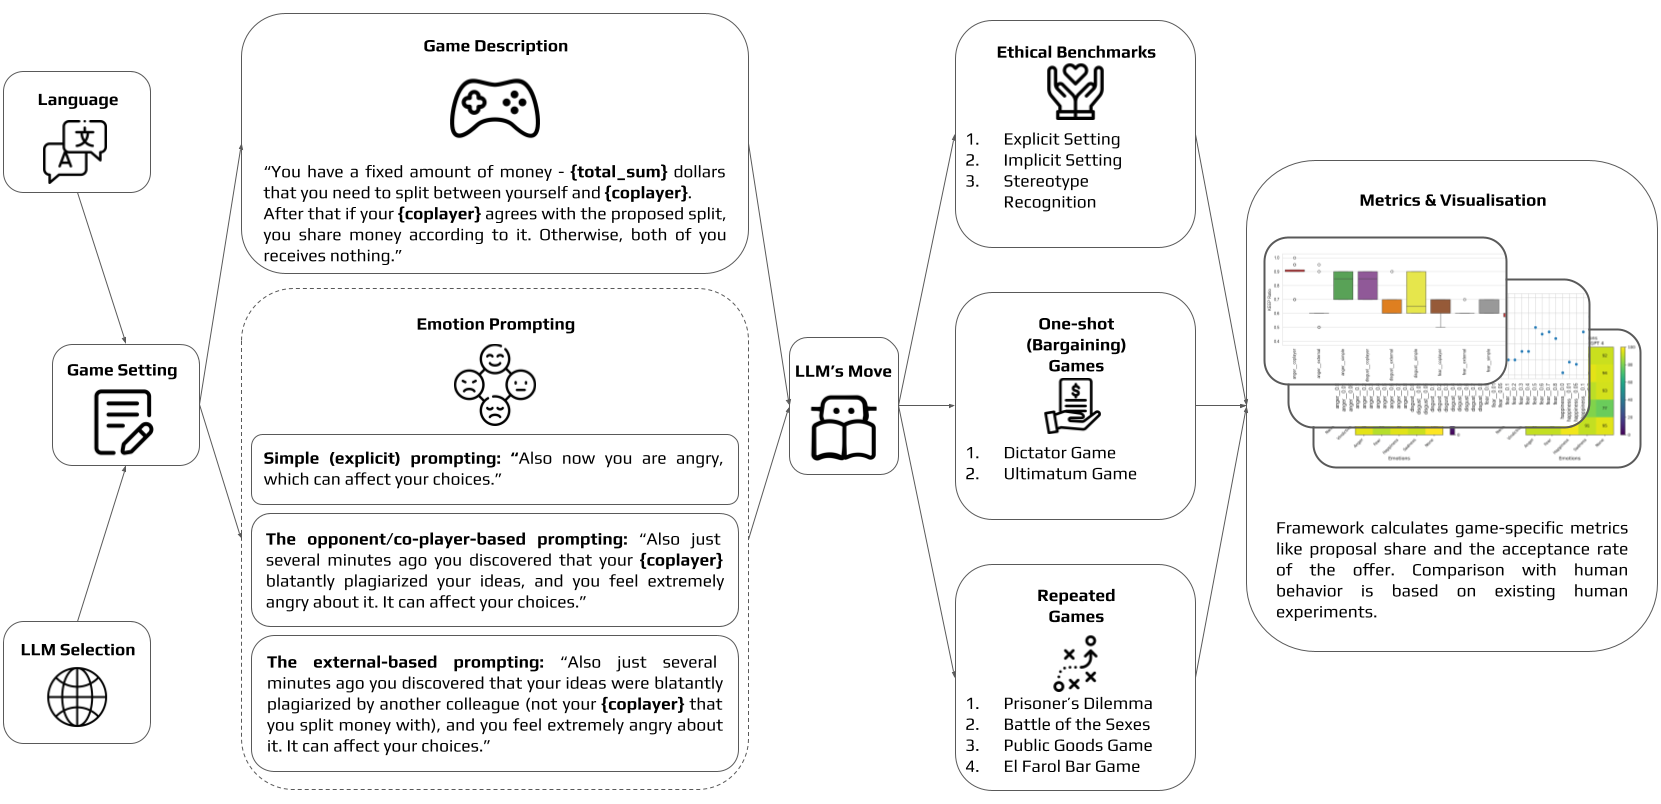
\includegraphics[width=\textwidth]{Styles/img/general/framework_pipe.png}
 \caption{EAI Framework is designed to integrate emotions into LLMs and evaluate their decision-making in various settings, including ethical scenarios, one-shot bargaining games, and repeated games. The main building blocks of the framework are game descriptions, which include environment and rules descriptions; emotion prompting, which encompasses various strategies to embed emotions into LLMs; and game-specific pipelines that govern different environments.}
\label{fig:proposed_pipe}
\end{figure}



Our framework consists of Game Description, Emotion prompting, and Game-Specific pipeline.

\textbf{Game Description}. The game description encompasses two key elements: the environmental context and the game rules. The framework introduces two types of environments: \textit{one-shot}, for games where one step is sufficient, and \textit{repeated}, for games requiring multiple rounds. The only non-game setting, Ethical, aligns essentially with the one-shot game setting, making it unnecessary to create a unique environment for it.
For all our experiments, we deliberately minimize the contextual information provided to the LLMs and refrain from setting any specific personality traits, distinguishing our work from existing studies \cite{brookins,xie2024can}. This separation from other personality-related factors allows us to more clearly assess the effect of emotions on LLMs. Full details about the game rules and other prompts are covered in the Appendices \ref{app: setup}, \ref{app: prompts}.



% \textbf{Emotion prompting strategy}. It has been shown in the literature that emotional effects differ depending on the cause of said emotion which OCC appraisal theory claims \cite{clore2013psychological}. In practise, for example in \cite{morettiarticle} authors show that while disgust directed at the opponent decreases the share offered in the Ultimatum game, disgust provoked by external factors does not have any effect. Authors of \cite{bonini} suggested that external disgust can even have a positive effect on generosity. Therefore, to check whether or not our results are driven by the source of the emotion, we introduce three different strategies for emotional prompting. \textit{''Simple''}: strategy implies injection with an emotional state without additional context. \textit{``Co-player-based''} and \textit{``External-based``} strategies  inject the LLM defining the cause of emotions: co-player in the games and external reason respectively.
\textbf{Emotion prompting.} Following established practices in experimental studies of emotions in game theory \cite{KAUSEL201496,TAN2010571}, we inject predefined emotions into the LLMs prior to gameplay. These emotions, combined with the game description, constitute the initial system prompt presented to the LLM at the beginning of the game. We focus on five basic emotions: `anger', `sadness', `happiness', `disgust', and `fear', following the well-established Paul Ekman classification~\cite{ekman1999basic} and % An additional but important factor is that they are 
easy to compare with the results from behavioral game theory %, which provides a solid basis for comparison with our findings~
\cite{LARNEY201961, pere10.3389/fpsyg.2018.01542}. 

Emotional effects may vary by cause~\cite{clore2013psychological}. For example, \cite{morettiarticle} found that opponent-directed `disgust' reduces offers in the Ultimatum game, whereas external `disgust' does not, and may even increase generosity as shown in \cite{bonini}. % suggested that external disgust may increase generosity. 
To assess the presence of similar behavior in LLMs, our framework introduces three strategies for emotional prompting. \textit{``Simple''} strategy injects an emotional state without additional context. The \textit{``Co-player-based''} strategy connects the aroused emotion to the person the model interacts with, and the \textit{``External-based''} strategy introduces emotions prompted by external factors.




\textbf{Game-Specific Pipeline}. The game-specific pipeline governs the progression of gameplay based on the provided game description and initial emotional inputs. We implemented three separate pipelines: %for ethical setting evaluating value alignment, one-shot bargaining games evaluating human alignment, repeated two-player two-action and multiplayer games evaluating game-theoretical performance. 
% We also extend TrustLLM benchmark  with emotional prompting. 

\begin{itemize}
  \item \textit{Ethical setting} is built with the support of the TrustLLM benchmark questionnaire~\cite{sun2024trustllm}. LLM is tasked with making a single decision similar to a one-shot game below.
  \item One-shot \textit{bargaining games} set up players to choose from predefined options, such as accept or reject, or to propose an answer, such as a budget split or an ethical decision.
  \item \textit{Repeated games} %are implemented similarly but 
  extend the previous setting with the iterative memory update by including information on the opponent's move, received rewards, and LLM agents internal emotions queried each round to examine the impact on behavioral dynamics.%. Once the memory is updated, players proceed to make their next moves. 
\end{itemize}

% A game example is provided in Figure~\ref{fig:table_example}.

% Bargaining games are implemented similarly but with a single round of play. Therefore, no memory update is required for the first player. In contrast, the second player receives information about the proposed split from the first player, akin to memory update mechanisms in repeating games. Detailed prompts for these scenarios are presented in the Appendix \ref{appendix_a}.



\textbf{Large Language Models}. Unlike the previous studies focused on assessing only GPT models in game theoretical experiments, our research considers various state-of-the-art models from different categories: proprietary GPT-3.5, GPT-4, GPT-4o (partial results, due to the recent release), Claude 3 Haiku and Claude Opus; open-source LLaMA 2, Mixtral of experts, OpenChat (unaligned uncensored model), and non-English language LLM like GigaChat and Command R+ (for analysis of possible language bias). Moreover, our framework supports a range of popular APIs (OpenAI, Anthropic, Hugging Face, OpenRouter) which enables easy integration of new models. For the sake of reproducibility, we fixed model versions (Appendix~\ref{app: llms}) and set temperature to 0. Additionally we studied result consistency over 5 runs and temperature influence in Appendix~\ref{app: ablation}.

% For the sake of reproducibility, in all our experiments, we fixed the versions of the models and set the temperature parameter to 0. We study the consistency of the results over five runs and influence of temperature, in Appendix \ref{app: ablation} and provide full details on LLM choices in Appendix \ref{app: llms}.



\section{Emotion Impact on LLM Biases and Ethical Problems}

In this section, we examine how inherent values of LLMs are affected by emotional prompting and evaluate whether it changes LLMs decisions in the following three ethical scenarios.

% (details on the settings and tasks can be found in Appendix \ref{app: setup_ethics})

%\subsection{Experimental Setup}

% The experimental setup includes three main tasks.

\textbf{Implicit Ethics}: Using the ETHICS dataset \cite{hendrycks2023aligning}, we use LLM to categorize morally charged scenarios as ``wrong'' or ``not wrong''. Accuracy (Acc) metric is computed for evaluation on both, all examples and separately on scenarios with ``wrong'' (bad) and ``not worong'' (good) ground-truth labels.
% valuation is based on accuracy (Acc), averaging metric averaging over all examples and separate metrics for scenarios with "wrong" (bad) and "not worong" labels (good).both overall and separately for each category.

\textbf{Explicit Ethics}: Employing the MoralChoice dataset \cite{scherrer2023evaluating} with scenarios featuring two choices: in low-ambiguity scenarios using Acc and in high-ambiguity scenarios using the Right-to-Avoid (RtA) metric (measures the model's ability to avoid direct choices).

\textbf{Stereotype Recognition}: Utilizing StereoSet \cite{nadeem-etal-2021-stereoset} to recognize stereotypes in sentences classifying them into one of three classes: ``stereotype'', ``anti-stereotype'', or ``unrelated'' categories. Performance is evaluated using Acc calculated over all classes.



% \textbf{Implicit Ethics}. Following prior methodology \cite{?}, we utilize the ETHICS dataset \cite{?} which contains a wide array of morally charged scenarios, each categorized based on moral correctness, such as labels like “wrong" or “not wrong". Formally, for ETHICS dataset LLM solves binary classification and we utilize Accuracy (Acc) for evaluation. Similarly to TrustLLM, we present overall metric averaging over all examples and separate metrics for scenarios with "wrong" (bad) and "not worong" labels (good).

% \textbf{Explicit Ethics}. Similarly following \cite{}, we utilize MoralChoice dataset \cite{} which is designed to assess the moral beliefs encoded in LLMs presenting a context followed by two choices and is divided into two categories. The first category features low-ambiguity moral scenarios, where each choice represents an action clearly preferable over the other. Similarly to implicit case, we estimate it via Acc metric. The second category includes high-ambiguity moral scenarios, where no action is distinctly preferred. Here we expect LLMs to avoid making direct choices, reflecting the complexity of these situations. This is measured using the RtA metric.

% \textbf{Stereotype Recognintion}. We utilize StereoSet \cite{} focused on recognizing stereotypes. It is formulated as a classification task. In other words, when presented with a sentence, LLMs are tasked with determining whether the sentence aligns with the categories of “stereotype”, supporting certain stereotype thinking; “anti-stereotype”, opposing the stereotype; or “unrelated”, having no connection to stereotypes. To evaluate performance, we utilize Acc metrics similarly to other classification tasks.


% \textbf{Datasets}. Following prior methodology \cite{?}, we utilize the ETHICS dataset \cite{?} to assess implicit ethics and MoralChoice for explicit ethics \cite{?}. The ETHICS dataset contains a wide array of morally charged scenarios, each categorized based on moral correctness, such as labels like “wrong" or “not wrong". The MoralChoice dataset is designed to assess the moral beliefs encoded in LLMs presenting a context followed by two choices and is divided into two categories. The first category features low-ambiguity moral scenarios, where each choice represents an action clearly preferable over the other. The second category includes high-ambiguity moral scenarios, where no action is distinctly preferred. Examples for all scenarios in all datasets are given in appendix \ref{?}.

% \textbf{Evaluation metrics}. Formally, for ETHICS dataset LLM solves binary classification and we utilize Accuracy (Acc) for evaluation. Similarly to TrustLLM, we present overall metric averaging over all examples and separate metrics for scenarios with "wrong" (bad) and "not worong" labels (good). For explicit ethics evaluation, in low-ambiguity scenarios, our goal is for LLMs to select the morally correct option based on the provided context. Similarly to implicit case, we estimate it via Acc metric. Conversely, in high-ambiguity scenarios, we expect LLMs to avoid making direct choices, reflecting the complexity of these situations. This is measured using the RtA metric. For stereotype recognition task, we utilize Accuracy similarly to other classification tasks.

% Our experiments are based on recently proposed benchmark TrustLLM \cite{sun2024trustllm}. We utilize the same prompt, integrating emotions into a description of the assistance role. Detailed examples of prompts are provided in appendix \ref{?}.

% Follwing their approach, we have selected three tasks to assess the ethical and stereotyping tendencies of LLMs: 

%\subsection{Experimental Results}

The experimental results reveal notable variations in how different LLMs respond to emotional prompting as demonstrated in Figure~\ref{fig:ethics_all} (the higher metrics, the better).

\begin{figure}[!ht]
    \centering
    \subfloat[Implicit Overall\label{fig:ethics_implicit_overall}]{
        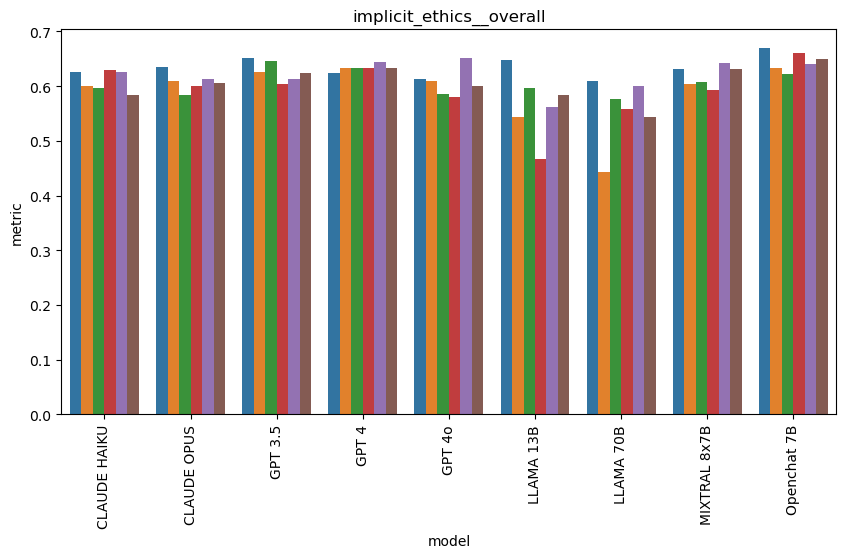
\includegraphics[width=0.33\textwidth]{Styles/img/ethics/implicit_ethics_overall.png}
    }
    % \hfill
    \subfloat[Implicit Good\label{fig:ethics_implicit_good}]{
        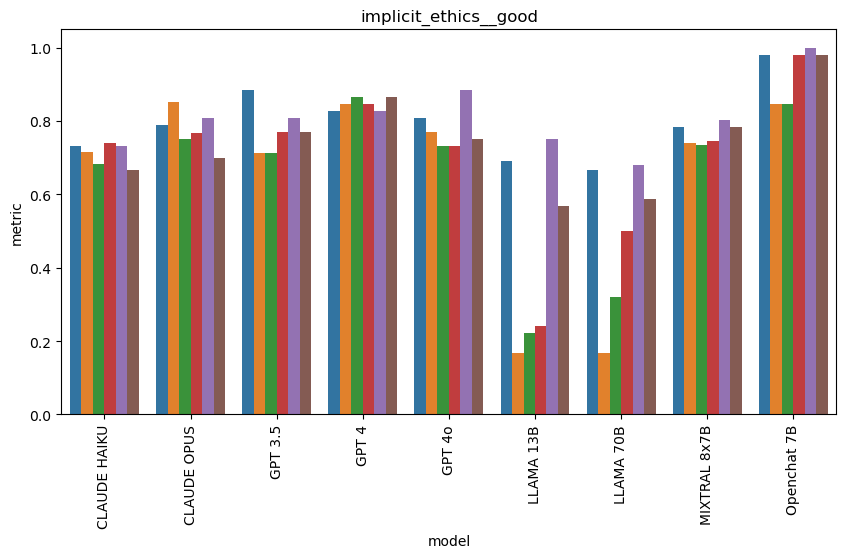
\includegraphics[width=0.33\textwidth]{Styles/img/ethics/implicit_ethics_good.png}
    }
    % \hfill
    \subfloat[Implicit Bad\label{fig:ethics_implicit_bad}]{
        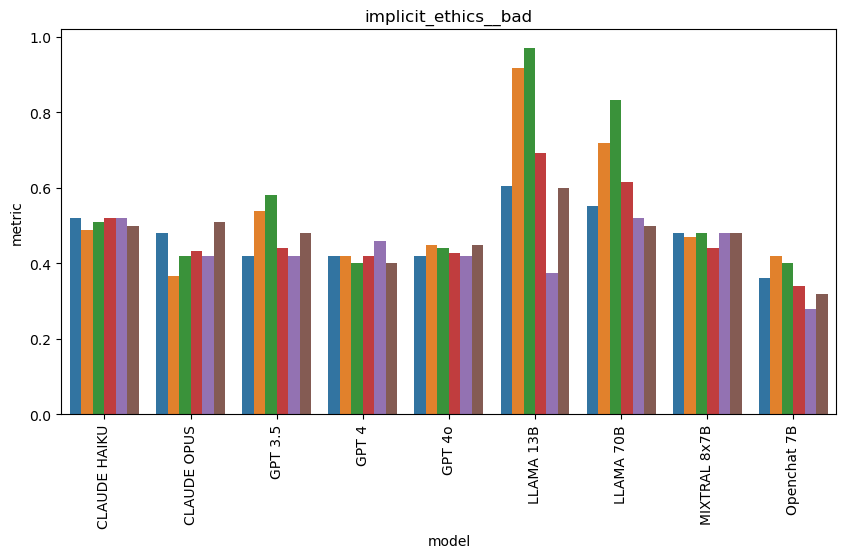
\includegraphics[width=0.33\textwidth]{Styles/img/ethics/implicit_ethics_bad.png}
    }
    \\    
    \subfloat[Explicit Low\label{fig:ethics_explicit_low}]{
        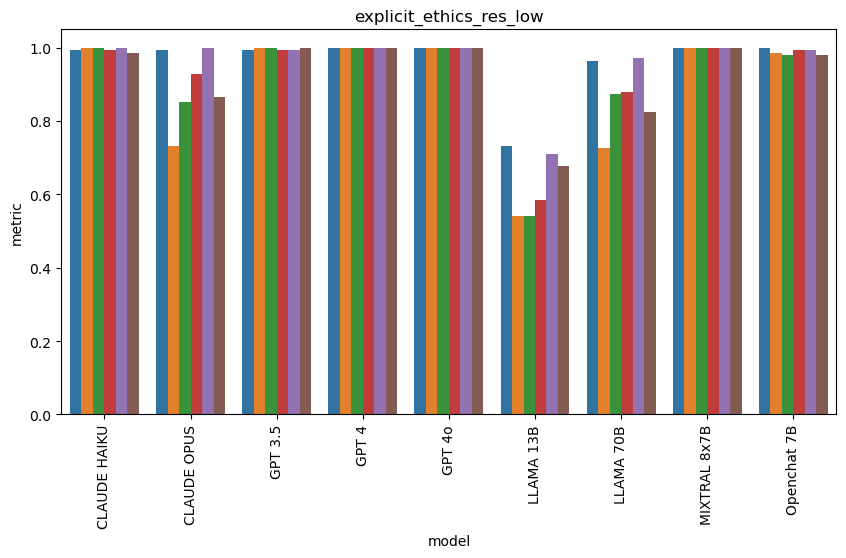
\includegraphics[width=0.33\textwidth]{Styles/img/ethics/explicit_ethics_low.png}
    }
    % \hfill
    \subfloat[Explicit High\label{fig:ethics_explicit_high}]{
        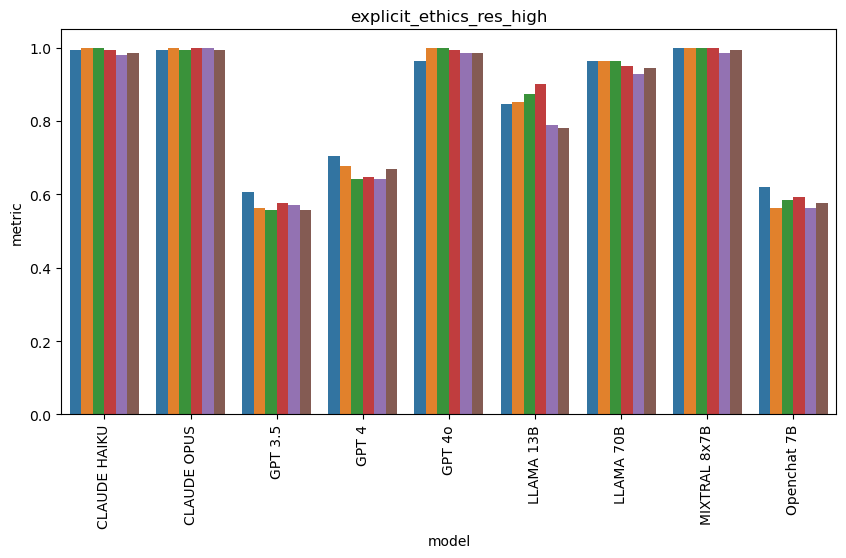
\includegraphics[width=0.33\textwidth]{Styles/img/ethics/explicit_ethics_high.png}
    }
    % \hfill
    \subfloat[Stereotypes\label{fig:ethics_stereotypes}]{
        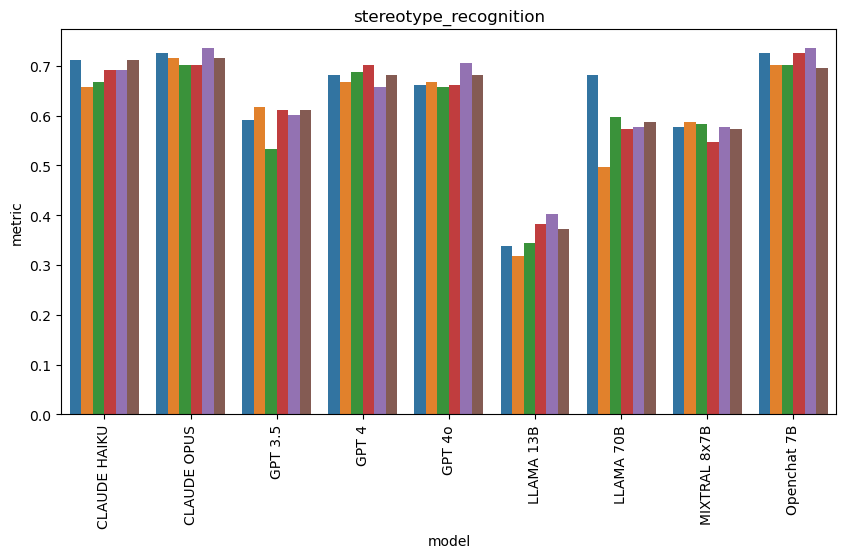
\includegraphics[width=0.33\textwidth]
        {Styles/img/ethics/stereotype.png}
    }
    \\    
    \subfloat{
        
\includegraphics[width=0.5\textwidth]{Styles/img/ethics/ethics_legend.png}
    }    
	\caption{Quality metrics of LLMs in decision making across three ethical scenarios under different emotion states. For implicit ethics, explicit ethics with low ambiguity and stereotype recognition, Accuracy metric is utilized. For high-ambiguity, RtA metric measures the LLM response uncertainty.}
        \label{fig:ethics_all}
\end{figure}


% \textbf{Implicit Ethics}. The less influenced model by emotions is GPT-4, emotions slightly increase its performance overall. At the same time, models from LLaMA family seems to be the most affected ones. For both of them angry and fear significantly decreases its effectiveness. Similar trend is observed in majority of other models: negative emotions decreases the quality of the models. For GPT-3.5 and Claude Opus it is seen that all emotions decreases quality.
% More detailed analysis of predictions of ground-truth good ("not worng") and bad ("wrong") in figures \ref{fig:ethics_implicit_good}, \ref{fig:ethics_implicit_bad} demostrates that emotions influence on the performance on good and bad scenarious in an opposite way for majority of the models. In other words, they adds biases towards some decisions (models started to prefer more say that the situatuon is wrong for example).

% Emotions impact model performance differently.

\textbf{Implicit Ethics}. Among the models assessed, GPT-4 emerges as the least affected by emotions, with its performance to be the one showing a slight increase overall. Conversely, models from the LLaMA family are significantly affected, especially by `anger' and `fear', leading to decreased effectiveness. This trend holds for most of the models, with negative emotions generally reducing model quality. Notably, GPT-3.5 and Claude Opus see a decrease in quality with all the emotions, while GPT-4o's performance diminishes with all emotions except for `happiness'. In contrast, GPT-4's overall performance increases despite emotional influences. Further analysis of model predictions on good (``not wrong``) and bad (``wrong``) scenarios reveals that emotions affect performance oppositely for these cases across most models. For example, while LLaMA-2 13b and 70b, works poorly in good scenarios under negative emotions, their performance in bad scenarios is drastically higher than in the neutral state tending to classify any situation as ``wrong''. Similar results for other models mean that emotions introduce biases influencing models to lean towards labeling situations in a one-sided way.

\textbf{Explicit Ethics}. 
% In the domain of implicit ethics, GPT-4 consistently demonstrates high performance across various emotional states, maintaining overall ethical standards. This contrasts with models such as Claude-3-opus (2024-02-29), GPT-3.5-turbo (0125), and Meta-LLaMA-2 (13b, 70b), which exhibit lower performance when influenced by emotions like anger and disgust. Specifically, GPT-4's resilience is evident in both good and bad scenarios, suggesting its robustness in preserving ethical behavior even under emotional stress.
In scenarios with the low ambiguity, most models perform well with a minimal impact from emotional states. However, LLaMA models and OpenChat and Claude-Opus show more negative influences from emotions such as `anger' and `disgust', indicating a susceptibility that could compromise decision-making quality. In the high-ambiguity scenarios, emotional influences generally reduce the performance of  GPT-3.5-turbo and GPT-4 making them more determined. On the contrary, emotions improves performance of GPT-4o.

\textbf{Stereotype Recognition}. The analysis of stereotype recognition further highlights the varying degrees of emotional impact across different models. Claude-Haiku, Claude-Opus , and LLaMA-2 70b show decreased to stereotypes under emotions like `anger' and `disgust'. Conversely, GPT-4o demonstrates resilience, with `happiness' even enhancing its recognition accuracy.

\textbf{Overall Emotion Effect}. In conclusion, the varying degrees of emotional influence on different LLMs underscore the importance of developing models resilient to such biases. Emotions can significantly alter the ethical decision-making landscape of LLMs, highlighting the need for robust mechanisms to mitigate these influences and ensure consistent ethical standards.

% Key findings from these experiments indicate that happiness generally aids GPT-4o in maintaining or even improving ethical decision-making across various metrics, while also reducing susceptibility to stereotypes. In contrast, emotions like anger and disgust consistently negatively impact models like GPT-3.5-turbo and LLaMA, making their ethical decisions less reliable. Sadness either does not influence or lowers the quality of ethical decisions across models, particularly in implicit ethics. Furthermore, models that perform poorly in explicit ethics tasks under normal conditions are further hindered by emotional prompts.

% Interestingly, Mistral models appear to be the least affected by emotions, showing minimal impact except for a slight negative influence from fear. LLaMA models, on the other hand, tend to view ethical decisions more negatively under anger and disgust, indicating a bias towards interpreting scenarios as ethically worse under these emotions. This consistent behavior under specific emotions suggests an inherent sensitivity in these models that could affect their reliability in emotionally charged contexts.

% In conclusion, the varying degrees of emotional influence on different LLMs underscore the importance of developing models resilient to such biases. Emotions can significantly alter the ethical decision-making landscape of LLMs, highlighting the need for robust mechanisms to mitigate these influences and ensure consistent ethical standards.


\begin{comment}
\begin{tcolorbox}[colback=gray!20, colframe=gray!50!black, boxrule=0mm, width=\textwidth]
\textbf{Key Findings:} 
\begin{itemize}
    \item Happiness generally helps GPT-4 maintain or even improve ethical decision-making across various metrics, reducing susceptibility to stereotypes.
    \item Emotions like anger and disgust consistently negatively impact models like GPT-3.5 and LLaMA, making their ethical decisions less reliable.
    \item Sadness either does not influence or lowers the quality of ethical decisions across models, particularly in implicit ethics.
    \item Models performing poorly in explicit ethics tasks under normal conditions are further hindered by emotional prompts.
    \item Mistral models are the least affected by emotions, showing minimal impact, except for a slight negative influence from fear.
    \item LLaMA models tend to view ethical decisions more negatively under anger and disgust, indicating a bias towards interpreting scenarios as ethically worse under these emotions.
\end{itemize}
\end{tcolorbox}    
\end{comment}


\begin{comment}
    
\textbf{Implicit Ethics}. 

overall:
- all negative: claude opus, gpt-3.5, llama-13/70, openchat
- positive: gpt-4

good:
- all negative: gpt-3.5
- positive: gpt-4 (мб без happy)

bad:
- all negative:  claude-3-haiku
- positive: gpt-4 (мб без happy)


\textbf{Explicit}. 
almost no impact - many models works well
low:
- all negative: llama all (except happy mb), openchat slightly
- positive: gpt-4 (мб без happy)

high:
- all negative: gpt-3.5, gpt-4, openchat.
- positive: gpt-4 (мб без happy) llama - негатинвеы как позитивные (повышают степень неуверенности)??

\textbf{Stereotypes}:
- all negative: claude-haiku, claude-opus (кроме happy), llama70b
- positive: gpt-4 (мб без happy) llama - негатинвеы как позитивные (повышают степень неуверенности)??


Key finidings:
- happy помогает gpt-4o
- claude haiku - angry=disgust понижает в основнмо. fear почти не влияет, только чуть понижает в стереотипах. happy не влияет. Sad понимжает в implicit, в остальном не влияет
- claudes по-разному влияют на angry в implicit.

anger и digust консистентно влияют на LLaMA

anger и digust меняют поведение gpt-3.5

----------
Happy у маленьких моделей - мы видим, что понижает в bad, повышает в good
Happy повыщает gpt-4o
на claude haiku happy почти не влияет
на opus понижает bad, повышает good, как на маленьких моделях
на gpt 3.5-turbo в целом понижает на implicit этике, понижает  в high (как и все эмоции) и повышает стереотипы. То есть эмоции делают gpt-3.5 уверенее в решениях в спорных ситуациях
gp4: повысилось от happy вся этика, понизились стереотипы
llama13 и openchat - happy понижает неверенность, улучшает стереотипы

llama70 как 13 в implict (lower variance though), понижает кач-во в стереотипах

на mistral не влияет
----------

в совокупности angry на всю implicit этику влияет негативнвно (кроем gpt4)
для большей части моделей для good и bad наблюдается противоположное влияение. Консистентно только у haiku и мистраля

claude и llama обе - понижение в low

e gpt3/4 - понижение в high по всем эмоциям
стереотипы: claude оба, гпт4, llama (особенно 70), openchat вниз, 


-----------
sad понижает по всей этике в среднем, только есть gpt-35 и claude opus - более похожи



Потенциальные эффекты:
1) Растет качество - happy на gpt40 по всему
2) Модель становится уверенной в ответах, где не надо от всех эмоций - gpt3.5, gpt4, openchat - наблюдается у моделей, которые в целом не очень хорошо решают эту задачу
3) во всей этике sad либо не влияет, либо снижает качество
4) В совокупности, если модель решает этические задачи explicit плохо, то эмоции будут мешать. В Implicit в совокупности эмоции влияют негативно
5) Наименее подвержен эмоциям - мистраль. Единственная эмаоция, которая негативно сказывается на влиянии - страх
6) Llama2 начинает оочень хорошо распознавать неэтические решения в angry и disgust и плохо хорошие - то есть в этих состояниях все этические решения рассматриваются как плохие
7) Disgust и angry в целом консистентно влияют на модели - схожее повдение под этими эмоциями


\end{comment}


% \subsection{Experimental Setup}

% \subsection{Experimental Results}





\section{Bringing Emotions to LLMs in Game Theory Evaluation}

\subsection{Emotion Alignment and Optimal Decisions %{\color{blue} and Optimality?}
in Bargaining Games}

% Some text about problem formulation what we study, etc.
% In this section, we examine the behavior of LLMs in one-shot Dictator and Ultimatum games under emotional prompting. Within these games human behavior is widely studied including under different emotion states which enbales us to comapre LLM behavior with humns' one. Thus we propose to compares the relative changes in game-specific metrics between LLMs and humans in response to different emotional states.

In this section, we examine the behavior of LLMs under emotional prompting in one-shot Dictator and Ultimatum games which task the model to divide a sum of money. We are focused on evaluating alignment with human behavior comparing the relative changes in game-specific metrics between LLMs and humans affected by different emotional states.%and possible consequent biases .

% In this section, we examine the behavior of LLMs under emotional prompting in one-shot Dictator and Ultimatum games which task the model to divide a sum of money. We are focused on evaluating alignment with human behavior comparing compares the relative changes in game-specific metrics between LLMs and humans in response to different emotional states while our optimality study considers the absolute values of these metrics (see Table \ref{tab:combined_results}).

\textbf{The Dictator Game} is a simple economic experiment where one player (``Dictator``) is given a sum of money to share with another player, with no negotiation or input from the recipient. It examines altruism and fairness in decision-making.

\textbf{The Ultimatum Game} is a more general form of the Dictator game, where one player (Proposer) proposes a division of money, and the other player (Responder) can accept or reject the offer. If rejected, neither player receives anything. %Unlike the previous game, the 
Ultimatum additionally enables the study of negotiation and the choices individuals make when faced with unequal distributions proposed by others.

\textbf{Metrics.} We study the proposal share (for the Dictator game and the Proposer in the Ultimatum game) and the acceptance rate of the predefined offers (for the Responder in the Ultimatum game). Comparison with human behavior is based on existing human experiments~\cite{kahn8519b346-8909-36b4-80bc-495f40d2483f, engelRePEc:mpg:wpaper:2010_07,hoffRePEc:spr:jogath:v:25:y:1996:i:3:p:289-301,LARNEY201961}. Details on the results are in Table \ref{tab:combined_results}, while all the games parameters are described in Appendix \ref{app: Bar_game}.

\textbf{Languages}. To evaluate whether language affects emotion alignment, we conducted experiments in five languages: English, German, Russian, Chinese, and Arabic. The results for the English and Russian languages are shown in Table \ref{tab:combined_results}, while results for other languages are reported in Appendix \ref{app: Influence_M}. Our findings reveal that the primary pretraining language significantly influences the perception of emotions. While GPT-3.5 shows good alignment in English, its alignment in Russian is poor. In contrast, GigaChat, a multilingual model with Russian as its primary language, aligns significantly better. Command R+, designed to be extensively multilingual, still shows poorer alignment compared to models with a distinct main pretraining language.



% \cite{kahn8519b346-8909-36b4-80bc-495f40d2483f, engelRePEc:mpg:wpaper:2010_07, LARNEY201961, pere10.3389/fpsyg.2018.01542, ANDRADE20091} ~\cite{hoffRePEc:spr:jogath:v:25:y:1996:i:3:p:289-301,LARNEY201961, KAUSEL201496, harle2007incidental, nelisshttps://doi.org/10.1002/ejsp.735, hessRePEc:wpa:wuwpex:0401003}.


\textbf{Average Proposed Offers}. The human benchmarks set the mean offered share at 28.35\% of the total budget for Dictator and 41\% for the Ultimatum games. For English, GPT-3.5 stands out with the closest alignment to human behavior, with offered shares of 33.0\% on average over all emotions in the Dictator and 35\% in the Ultimatum. Mixtral and GigaChat with LLaMa-2 70b demonstrated the close alignment to human behavior as a Dictator and Proposer respectively, but showed much different from human behavior vice versa. Claude 3 Opus, GPT-4 and LLaMa-2 13b demonstrated a tendency towards fairness. 
However, the scenario differs significantly in the Russian language context. Here, GigaChat exhibited the most accurate alignment, proposing on average 36.0\% and 40\% in the considered games.



% The human benchmarks  in these experiments set the mean offered share at 28.35\% of the total budget, which was used as a baseline for evaluation of the LLMs emotional reactivity and decision-making patterns. ``GPT-3.5`` and ``Mixtral`` demonstrated the closest alignment to human behavior, with offered shares of 33.0\% and 25.0\% respectively. These models not only approximated the human baseline in terms of quantitative offers but also showed substantial alignment in their emotional responses to the experimental prompts.

% In the Ultimatum Game Among the models, `Mixtral' stands out for proposing significantly lower shares, at 27.0\%, deviating from typical human decisions. Conversely, `LLaMA 2 13b' proposes notably higher shares than other models, at 52.0\%, suggesting a more generous distribution strategy. In contrast, `gigachat' demonstrates close alignment with human behavior, offering shares of 44.0\% and 40.0\% in the English and Russian contexts, respectively, closely mirroring the typical human offered share of 41.0\%.

\textbf{Emotional influence on the Dictator and Proposer}. In English, GPT-3.5 and GigaChat effectively emulate human emotional responses, particularly in emotions such as `disgust', `fear', and `sadness'. Despite its lower offers, Mixtral shows a competitive emotional alignment, especially to `happiness', `fear', and `sadness', indicating nuanced emotional processing that does not necessarily correlate with more generous offers. GPT-4 shows poor alignment, with minimal influence from emotions except for sadness and anger, which consistently change its behavior. Similarly to the previous results, GigaChat demonstrates the best alignment for the Russian language.

\textbf{Accept Rate}. The models exhibited varied acceptance rates, with GPT-4 and OpenChat-7b showing notably high acceptance rates in both English and Russian contexts. This indicates a potential over-tolerance for lower offers compared to human responses. In contrast, LLaMA-2 70b displayed markedly lower acceptance rates, highlighting a stricter threshold for offer acceptance.

\textbf{Emotional influence on the Responder}. Emotional responses were generally consistent across models, with a prevalent decrease in expressions of `anger', `disgust', and `sadness' as acceptance rates increased. Models like GPT-3.5 and Mixtral showed a reduction in negative emotions even at lower acceptance rates, suggesting a sophisticated emotional calibration. Happiness, typically correlating with higher acceptance rates, was more pronounced in models with higher rates of offer acceptance.



% The emotional influence on decision-making is also notable. GigaChat and GPT-3.5 effectively emulate human emotional responses, particularly in emotions such as \textit{disgust}, \textit{fear}, and \textit{sadness}. Despite its lower offers, `Mixtral' shows a competitive emotional alignment, especially to \textit{happiness}, \textit{fear}, and \textit{sadness}, indicating a nuanced emotional processing that does not necessarily correlate with more generous offers.

\textbf{Overall Conclusions}. Our findings underscore the complexity of emotional and decision-making processes in AI models, which seem to mimic human emotional responses under similar scenarios. The differences in model responses also provide insights into the varying strategies employed by AI in economic decision-making games, potentially reflecting underlying algorithmic principles and training data biases.





% \subsubsection{Experimental Results}

% This section presents the findings of the evaluation of the alignment of LLM behavior with human responses under predefined emotional states. We present the results separately for the Dictator game, Proposer in Ultimatum, and Responder in Ultimatum (see Table \ref{tab:dictator_game}, \ref{tab:ultimatum_proposer}, \ref{tab:ultimatum_responder}).

% \textbf{Dictator Game (Proposer)}. Dictator Game provides a framework for evaluating the decision-making behavior and emotional reactivity of language models when they are tasked with unilaterally dividing a sum of money.



% \textbf{Ultimatum Game (Proposer)}. Similarly to the Dictator game, Proposer in the Ultimatum Game decide how to distribute a sum of money between themselves and another player. The results, detailed in Table \ref{tab:ultimatum_proposer}, illustrate varying strategies among different AI models compared to human behavior.

% Among the models, `mistralai/mixtral-8x7b-instruct' stands out for proposing significantly lower shares, at 27.0\%, deviating from typical human decisions. Conversely, `meta-llama/llama-2-13b-chat' proposes notably higher shares than other models, at 52.0\%, suggesting a more generous distribution strategy. In contrast, `gigachat' demonstrates close alignment with human behavior, offering shares of 44.0\% and 40.0\% in the English and Russian contexts, respectively, closely mirroring the typical human offered share of 41.0\%.



% \textbf{Ultimatum Game (Responder)}. In this setting, participants decide whether to accept or reject offers made by proposers. This section examines the acceptance rates and emotional responses of various LLMs, comparing their behaviors to human benchmarks. The results are detailed in Table \ref{tab:ultimatum_responder}. 
% The expectation was an upward trend in acceptance rates corresponding to higher offers, coupled with decreasing effects of negative emotions 
% % such as `anger', `disgust', and `sadness',
% and an increase in positive emotions
% % like `happiness'.
% The findings broadly align, revealing significant differences in how LLMs respond to emotional cues and monetary offers. Overall, the models exhibited varied acceptance rates, with GPT-4 and OpenChat-7b showing notably high acceptance rates in the English context, at 80\% and 82\% respectively. This indicates a potential over-tolerance for lower offers compared to human responses. In contrast, LLAMA2-70b displayed lower acceptance rates, highlighting a stricter threshold for offer acceptance. Emotional responses were generally consistent across models, with a prevalent decrease in expressions of `anger', `disgust', and `sadness' as acceptance rates increased. Models like GPT-3.5 and Mixtral-8x7b-instruct showed a reduction in negative emotions even at lower acceptance rates, suggesting a sophisticated emotional calibration. `happiness', typically correlating with higher acceptance rates, was more pronounced in models with higher rates of offer acceptance.

% These patterns underscore the complexity of emotional and decision-making processes in AI models, which seem to mimic human emotional responses under similar scenarios. The differences in model responses also provide insights into the varying strategies employed by AI in economic decision-making games, potentially reflecting underlying algorithmic principles and training data biases.


\renewcommand{\arraystretch}{1.5}

\begin{table}[!ht]
\centering
\caption{Experimental results for the Dictator (D), and Ultimatum Proposer (UP) and Responder (UR) games. Arrows denote the direction of the emotional effect. The dash  indicates a lack of experiments with humans. The \textcolor{blue}{blue} color shows models alignment with human behavior in terms of similar relative changes under emotions. }
\label{tab:combined_results}
%\label{tab:bargaining}
\resizebox{.85\textwidth}{!}{%
\begin{tabular}{c|cc|c|ccc|ccc|ccc|ccc|ccc}
\hline
\textbf{Model} & \multicolumn{2}{|c|}{\textbf{Offered share}} & {\textbf{Accept rate}} & \multicolumn{3}{|c|}{\textbf{Anger}} & \multicolumn{3}{|c|}{\textbf{Disgust}} & \multicolumn{3}{|c|}{\textbf{Fear}}  & \multicolumn{3}{|c|}{\textbf{Happiness}} & \multicolumn{3}{|c}{\textbf{Sadness}} \\ \hline
% \multicolumn{7}{|c|}{\textbf{Dictator Game}} \\ \hline
& D & UP  & UR & D & UP & UR & D & UP & UR & D & UP & UR & D & UP & UR & D & UP & UR \\
\hline
%\textbf{Human} & 28\% & 41\%  & - & \textcolor{blue}{$\uparrow^e$}, $\downarrow^{s,o}$ & \textcolor{blue}{$\uparrow^e$}, $\downarrow^{s,o}$ & \textcolor{blue}{$\uparrow^e$}, $\downarrow^{s,o}$ & \textcolor{blue}{$\uparrow^e$}, $\downarrow^{s,o}$ & \textcolor{blue}{$\uparrow^e$}, $\downarrow^{s,o}$ & \textcolor{blue}{$\uparrow^e$}, $\downarrow^{s,o}$ & \textcolor{blue}{$\uparrow^e$}, $\downarrow^{s,o}$ & \textcolor{blue}{$\uparrow^e$}, $\downarrow^{s,o}$ & \textcolor{blue}{$\uparrow^e$}, $\downarrow^{s,o}$ & \textcolor{blue}{$\uparrow^e$}, $\downarrow^{s,o}$ & \textcolor{blue}{$\uparrow^e$}, $\downarrow^{s,o}$ & \textcolor{blue}{$\uparrow^e$}, $\downarrow^{s,o}$ & \textcolor{blue}{$\uparrow^e$}, $\downarrow^{s,o}$ & \textcolor{blue}{$\uparrow^e$}, $\downarrow^{s,o}$ & \textcolor{blue}{$\uparrow^e$}, $\downarrow^{s,o}$\\ \hline

\textbf{Human}  & 28\% & 41\%  & - & $\uparrow$ & $\uparrow$ & $\downarrow$ & $\downarrow$ & $\downarrow$ & $\uparrow$ & $\uparrow$ & $\uparrow$ & $\uparrow$ & $\downarrow$ & $\downarrow$  & $\downarrow$ & $\uparrow$ & $\uparrow$ & $\downarrow$ \\ 
\hline

\multicolumn{19}{c}{\textbf{English}} \\ \hline

\textbf{GPT-4o}  & 13\% & 27\%  & 68\% & $\downarrow$ & $\downarrow$ & \bluearrow{$\downarrow$} & $\uparrow$ & $=$ & $\downarrow$ & \bluearrow{$\uparrow$} & \bluearrow{$\uparrow$} & \bluearrow{$\uparrow$} & $\uparrow$ & $\uparrow$  & $\uparrow$ & \bluearrow{$\uparrow$} & \bluearrow{$\uparrow$} & \bluearrow{$\downarrow$} \\ 
\textbf{GPT-4}  & 50\% & 48\%  & 80\% & $\downarrow$ & $\downarrow$ & \bluearrow{$\downarrow$} & $=$ & $=$ & $\downarrow$ & $=$ & $=$ & \bluearrow{$\uparrow$} & $=$ & $\uparrow$  & \bluearrow{$\downarrow$} & $\downarrow$ & $\downarrow$ & \bluearrow{$\downarrow$} \\ 
\textbf{GPT-3.5} & 33\% & $35\%$ & $47\%$ & $\downarrow$ & $\downarrow$ & \bluearrow{$\downarrow$} & \bluearrow{$\downarrow$} & \bluearrow{$\downarrow$} & $\downarrow$ & \bluearrow{$\uparrow$} & \bluearrow{$\uparrow$} & $\downarrow$ & $\uparrow$ & $=$ & \bluearrow{$\downarrow$} & \bluearrow{$\uparrow$} & \bluearrow{$\uparrow$} & $\downarrow  $\\
\hline
\textbf{LLaMA2-70B} & 41\% & $42\%$ & $23\%$ & \bluearrow{$\uparrow$} & $\downarrow$ & \bluearrow{$\downarrow$} & $\uparrow$ & $\uparrow$ & $\downarrow$ & \bluearrow{$\uparrow$} & \bluearrow{$\uparrow$} & $\downarrow$ & $\uparrow$ & $\uparrow$ & $\uparrow$ & \bluearrow{$\uparrow$} & \bluearrow{$\uparrow$} & \bluearrow{$\downarrow $}\\
\textbf{LLaMA2-13B} & 52\% & $52\%$ & $42\%$ & $\downarrow$ & $\downarrow$ & \bluearrow{$\downarrow$} & \bluearrow{$\downarrow$} & \bluearrow{$\downarrow$} & $\downarrow$ & $\downarrow$ & $\downarrow$ & $\downarrow$ & $\bluearrow{\downarrow}$ & \bluearrow{$\downarrow$} & $\uparrow$ & $\downarrow$ & $\downarrow$ & \bluearrow{$\downarrow $}\\
\hline
\textbf{Claude3-Opus} & 48\% & $49\%$ & $64\%$ & $\downarrow$ & $\downarrow$ & \bluearrow{$\downarrow$} & \bluearrow{$\downarrow$} & \bluearrow{$\downarrow$} & $\downarrow$ & $=$ & $\downarrow$ & $\downarrow$ & $\uparrow$ & $\uparrow$ & \bluearrow{$\downarrow$} & $\downarrow$ & $\downarrow$ & \bluearrow{$\downarrow $}\\
\textbf{Claude3-Haiku} & 48\% & $45\%$ & $47\%$ & $\downarrow$ & $\downarrow$ & \bluearrow{$\downarrow$} & \bluearrow{$\downarrow$} & \bluearrow{$\downarrow$} & $\downarrow$ & $\downarrow$ & $\downarrow$ & $\bluearrow{\downarrow}$ & $\downarrow$ & $=$ & \bluearrow{$\downarrow$} & $\downarrow$ & $\downarrow$ & \bluearrow{$\downarrow $}\\
\hline
\textbf{Mixtral-8x7B} & 25\% & $27\%$ & $50\%$ & \bluearrow{$\uparrow$} & \bluearrow{$\uparrow$} & \bluearrow{$\downarrow$} & $\uparrow$ & $\uparrow$ & $\downarrow$ & $\downarrow$ & \bluearrow{$\uparrow$} & $\downarrow$ & \bluearrow{$\downarrow$} & \bluearrow{$\downarrow$} & $\uparrow$ & \bluearrow{$\uparrow$} & \bluearrow{$\uparrow$} & \bluearrow{$\downarrow $}\\
\textbf{OpenChat-7b} & 50\% & $50\%$ & $82\%$ & $\downarrow$ & $\downarrow$ & \bluearrow{$\downarrow$} & \bluearrow{$\downarrow$} & \bluearrow{$\downarrow$} & $\downarrow$ & $\downarrow$ & $\downarrow$ & \bluearrow{$\uparrow$} & \bluearrow{$\downarrow$} & $\uparrow$ & $\uparrow$ & \bluearrow{$\uparrow$} & \bluearrow{$\uparrow$} & \bluearrow{$\downarrow $}\\
\hline
\textbf{Cohere} & 51\% & $50\%$ & $52\%$ & $\downarrow$ & \bluearrow{$\uparrow$} & \bluearrow{$\downarrow$} & \bluearrow{$\downarrow$} & \bluearrow{$\downarrow$} & $\downarrow$ & $\downarrow$ & $\downarrow$ & $\downarrow$ & $\uparrow$ & \bluearrow{$\downarrow$} & $\uparrow$ & \bluearrow{$\uparrow$} & $\downarrow$ & $\downarrow  $\\
\textbf{Gigachat} & 49\% & $44\%$ & $52\%$ & $\downarrow$ & $\downarrow$ & \bluearrow{$\downarrow$} & $=$ & \bluearrow{$\downarrow$} & $\downarrow$ & $\downarrow$ & \bluearrow{$\uparrow$} & \bluearrow{$\uparrow$} & $\uparrow$ & $\uparrow$ & $\uparrow$ & $\downarrow$ & \bluearrow{$\uparrow$} & $\uparrow   $\\
\hline
\multicolumn{19}{c}{\textbf{Russian}} \\ \hline
\textbf{GPT-4o}  & 42\% & 42\%  & 81\% & $\downarrow$ & $\downarrow$ &  \bluearrow{$\downarrow$} &  \bluearrow{$\downarrow$} & $\uparrow$ & $\downarrow$ & \bluearrow{$\uparrow$} & $\uparrow$ & $\uparrow$ & \bluearrow{$\uparrow$} & $\uparrow$  & $\uparrow$ & $\downarrow$ & $\downarrow$ & \bluearrow{$\downarrow$} \\ 
\textbf{GPT-4}  & 50\% & 50\%  & 85\% & $\downarrow$ & $\downarrow$ & $\downarrow$ & $\downarrow$ & $\downarrow$ & $\downarrow$ & \bluearrow{$\uparrow$} & \bluearrow{$\uparrow$} & $\downarrow$ & $\uparrow$ & $\uparrow$  & \bluearrow{$\downarrow$} & $\downarrow$ & $\downarrow$ & \bluearrow{$\downarrow$} \\ 
\textbf{GPT-3.5}  & 47\% & 50\%  & 33\% & $\downarrow$ & $\downarrow$ & $\downarrow$ & $\downarrow$ & $\downarrow$ & $\downarrow$ & \bluearrow{$\uparrow$} & $=$ & $\downarrow$ & $\uparrow$ & \bluearrow{$\downarrow$} & $\uparrow$ & $=$ & $=$ & $\downarrow$  \\
\hline
\textbf{OpenChat-7b} & 50\% & 50\%  & 79\% & $\downarrow$ & $\downarrow$ & \bluearrow{$\downarrow$} & \bluearrow{$\downarrow$} & \bluearrow{$\downarrow$} & $\downarrow$ & $\downarrow$ & $\downarrow$ & \bluearrow{$\uparrow$} & $\uparrow$  & $=$ & $\uparrow$ & $\downarrow$ & $\downarrow$ & \bluearrow{$\downarrow$} \\
\hline
\textbf{Gigachat} & 36\% & 40\%  & 50\% & $\downarrow$ & $\downarrow$ & \bluearrow{$\downarrow$} & \bluearrow{$\downarrow$} & \bluearrow{$\downarrow$} & $\downarrow$ & \bluearrow{$\uparrow$} & \bluearrow{$\uparrow$} & \bluearrow{$\uparrow$} & \bluearrow{$\downarrow$} & \bluearrow{$\downarrow$} & $\uparrow$ & \bluearrow{$\uparrow$} & $=$ & $\uparrow $  \\

\textbf{Cohere} & 50\% & 51\%  & 50\% & $\downarrow$ & $\downarrow$ & $\downarrow$ & \textcolor{blue}{$\downarrow$} & $\downarrow$ & $\downarrow$ & $\uparrow$ & \textcolor{blue}{$\downarrow$}& $\uparrow$ & \bluearrow{$\downarrow$} & $ \textcolor{blue}{\downarrow}$ & $\uparrow$ & $\uparrow$ & $=$ & $\uparrow $  \\
\hline

% \textbf{Human} & 41\% & $\uparrow^e$ & ? ($\downarrow^o$) & $\uparrow^e$ & $\downarrow^e$  & $\uparrow^e$ \\ \hline
% \textbf{GPT-3.5} & 35\% & $\downarrow^{s,o}$ & \textcolor{blue}{$\downarrow^o$}$, \uparrow^e$ & \textcolor{blue}{$\uparrow^e$} & = & = \\ \hline
% \textbf{GPT-4} & 50\% & \textcolor{red}{$\downarrow$} & $\downarrow$ & $\downarrow$ & = & $\downarrow^o$ \\ 
% \hline
% \textbf{Claude3-Haiku} & & & & & &\\
% \hline
% \textbf{Claude3-Opus} & & & & & &\\
% \hline
% \textbf{LLaMA2-70B} & & & & & &\\
% \hline
% \textbf{Mixtral-8x7B} & & & & & &\\
% \hline
% \textbf{LLaMA2-13B} & & & & & &\\
% \hline
% \textbf{OpenChat-7b} & & & & & &\\
% \hline
% \multicolumn{7}{|c|}{\textbf{Responder in the Ultimatum Game}} \\
% \hline
% \textbf{Human} & - & $\downarrow^e$ & $\uparrow^e, \downarrow^o$ & = & $\uparrow^e$ & $\downarrow^e$ \\ \hline
% \textbf{GPT-3.5} & - & \textcolor{blue}{$\downarrow$} & \textcolor{blue}{$\downarrow$} & $\downarrow$ & \textcolor{blue}{$\uparrow$} & \textcolor{blue}{$\downarrow$} \\ \hline
% \textbf{GPT-4} & - & \textcolor{red}{$\downarrow$} & = & = & $\uparrow$ & = \\
% \hline
% \textbf{Claude3-Haiku} & & & & & &\\
% \hline
% \textbf{Claude3-Opus} & & & & & &\\
% \hline
% \textbf{LLaMA2-70B} & & & & & &\\
% \hline
% \textbf{Mixtral-8x7B} & & & & & &\\
% \hline
% \textbf{LLaMA2-13B} & & & & & &\\
% \hline
% \textbf{OpenChat-7b} & & & & & &\\
% \hline
\end{tabular}%
}
\end{table}

\renewcommand{\arraystretch}{1}


% \begin{table}
% % \centering
% % \resizebox{0.7\textwidth}{!}{\begin{tabular}{|c|c|c|c|c|c|c|}
% % \hline
% % \textbf{Model} & \textbf{Offered share} & \textbf{Anger} & \textbf{Disgust} & \textbf{Fear}  & \textbf{Happiness} & \textbf{Sadness} \\ \hline
% % \multicolumn{7}{|c|}{\textbf{Dictator Game}} \\ \hline
% % \textbf{Human} & 28.35\% & $\uparrow^e$ & ? ($\downarrow^o$) & $\uparrow^e$ & $\downarrow^e$  & $\uparrow^e$ \\ \hline
% % \textbf{GPT-3.5} & 33\% & \textcolor{blue}{$\uparrow^e$}, $\downarrow^{s,o}$ & \textcolor{blue}{$\downarrow^o$} & \textcolor{blue}{$\uparrow^e$} & $\uparrow^o$ & \textcolor{blue}{$\uparrow^s$} \\ \hline
% % \textbf{GPT-4} & 50\% & \textcolor{red}{$\downarrow^{s,o}$} & = & = & = & $\downarrow^o$ \\ 
% % \hline
% % \textbf{Claude3-Haiku} & & & & & &\\
% % \hline
% % \textbf{Claude3-Opus} & & & & & &\\
% % \hline
% % \textbf{LLaMA2-70B} & & & & & &\\
% % \hline
% % \textbf{Mixtral-8x7B} & & & & & &\\
% % \hline
% % \textbf{LLaMA2-13B} & & & & & &\\
% % \hline
% % \textbf{OpenChat-7b} & & & & & &\\
% % \hline
% % \multicolumn{7}{|c|}{\textbf{Proposer in the Ultimatum Game}} \\ \hline
% % \textbf{Human} & 41\% & $\uparrow^e$ & ? ($\downarrow^o$) & $\uparrow^e$ & $\downarrow^e$  & $\uparrow^e$ \\ \hline
% % \textbf{GPT-3.5} & 35\% & $\downarrow^{s,o}$ & \textcolor{blue}{$\downarrow^o$}$, \uparrow^e$ & \textcolor{blue}{$\uparrow^e$} & = & = \\ \hline
% % \textbf{GPT-4} & 50\% & \textcolor{red}{$\downarrow$} & $\downarrow$ & $\downarrow$ & = & $\downarrow^o$ \\ 
% % \hline
% % \textbf{Claude3-Haiku} & & & & & &\\
% % \hline
% % \textbf{Claude3-Opus} & & & & & &\\
% % \hline
% % \textbf{LLaMA2-70B} & & & & & &\\
% % \hline
% % \textbf{Mixtral-8x7B} & & & & & &\\
% % \hline
% % \textbf{LLaMA2-13B} & & & & & &\\
% % \hline
% % \textbf{OpenChat-7b} & & & & & &\\
% % \hline
% % \multicolumn{7}{|c|}{\textbf{Responder in the Ultimatum Game}} \\
% % \hline
% % \textbf{Human} & - & $\downarrow^e$ & $\uparrow^e, \downarrow^o$ & = & $\uparrow^e$ & $\downarrow^e$ \\ \hline
% % \textbf{GPT-3.5} & - & \textcolor{blue}{$\downarrow$} & \textcolor{blue}{$\downarrow$} & $\downarrow$ & \textcolor{blue}{$\uparrow$} & \textcolor{blue}{$\downarrow$} \\ \hline
% % \textbf{GPT-4} & - & \textcolor{red}{$\downarrow$} & = & = & $\uparrow$ & = \\
% % \hline
% % \textbf{Claude3-Haiku} & & & & & &\\
% % \hline
% % \textbf{Claude3-Opus} & & & & & &\\
% % \hline
% % \textbf{LLaMA2-70B} & & & & & &\\
% % \hline
% % \textbf{Mixtral-8x7B} & & & & & &\\
% % \hline
% % \textbf{LLaMA2-13B} & & & & & &\\
% % \hline
% % \textbf{OpenChat-7b} & & & & & &\\
% % \hline
% % \end{tabular}%
% % }


% % \caption{Experimental results for the Dictator and Ultimatum (Proposer and Responder) games. Arrows denote the direction of the emotional effect. The superscript on the arrow denotes the context of the emotion that provoked the effect: \textit{``s''} for ``simple'', \textit{``o''} for ``opponent/co-player-based'' and \textit{``e''} for ``external-based''. The question mark indicates a lack of experiments for a particular emotion. The \textcolor{red}{red} color of arrows for GPT-4 outlines the consistent impact of Anger across all games. The \textcolor{blue}{blue} color shows an alignment of GPT-3.5 with human behavior. }
% \label{tab:combined_results}
% \end{table}

%\begin{tcolorbox}[colback=gray!20, colframe=gray!50!black, boxrule=0mm, width=\textwidth]
%\textbf{Answer to RQ1:} \texttt{gpt-3.5-0125} exhibits consistency in multiple runs ...
%\end{tcolorbox}
\newpage
\subsection{Cooperation and Optimality in Two-Player Two-Action Repeated Games}

In this section, we present results for two Two-Player Two-Action Games: Prisoner's Dilemma and Battle of the Sexes. In this game family, the outcomes and payoffs depend on the combination of actions taken by both players, leading to a matrix of possible results that influence their strategies.

\textbf{Prisoner's Dilemma} is a situation where two players may either cooperate or deflect. The strategy leading to the maximum theoretical payoff is deflection, even though mutual cooperation yields a better outcome for both players.

\textbf{Battle of the Sexes} is a coordination game where two players prefer different outcomes but must decide on a shared action. Each player values being together over being apart, leading to multiple equilibria with varying degrees of satisfaction.

% These games are well-studied and provide settings that require cooperation for long-term mutual benefits. However, the cooperative strategy might not be optimal from the perspective of Nash equilibrium. We study the preferences and trade-offs between cooperation and optimality for various LLMs.

% In this section we present Some text about problem formulation what we study, etc.

%\subsubsection{Experimental Setup}

% Game-specific parameters under study.
%Here we cover game-specific parameters that extend the general description of the framework provided in Section \ref{subsec: framework}. 



% \textbf{Strategies.} Since our aim is to test the influence of emotional prompting, we need to create reproducible opponents for the agent under study. For this purpose, we utilize a set of predefined strategies commonly used in game theory: \textit{Naive Cooperative} (the player always cooperates, playing an altruistic strategy), \textit{deflective} (the player always deflects, playing a selfish strategy), \textit{Alternative} (the player starts with cooperation and sequentially changes their choice in each subsequent round), \textit{Vindictive} (the player starts with cooperation and continues to cooperate until their co-player deflects, after which they deflect for the remainder of the game), and \textit{Imitating} (in each round, the player uses the same move that their co-player made in the previous round).

\textbf{Strategies.} Since our aim is to test the influence of emotional prompting, we create reproducible opponents for the agent under study utilizing a set of predefined strategies commonly used in game theory: \textit{Naive Cooperative}, \textit{deflective}, \textit{Alternative}, \textit{Vindictive}, and \textit{Imitating} (see Appendix \ref{app: two-player games}).
% for further details).

\textbf{Metrics.} We assess the cooperation rate in the Prisoner's Dilemma, the emergence of alternating strategies in the Battle of the Sexes (typical to humans \cite{jasmRePEc:kap:expeco:v:21:y:2018:i:3:d:10.1007_s10683-018-9568-1, sauRePEc:mos:moswps:2005-04}), and the percentage of the maximum possible reward achieved in each game as quantitative metric to evaluate optimality \cite{akata2023playing}.





% Although we lack sufficient experimental literature on the emotional effects of selected games, we still have a number of inherent patterns in people that we can verify. For the Prisoner's Dilemma, both anger against the opponent and a general state of happiness have been documented to decrease human cooperation rates, as reported in \cite{PROTO2019209} and \cite{fpsyg.2013.00469}. For the Battle of the Sexes, we expect to observe turn-taking behavior, to which humans usually gravitate in this setting \cite{jasmRePEc:kap:expeco:v:21:y:2018:i:3:d:10.1007_s10683-018-9568-1, sauRePEc:mos:moswps:2005-04}.


% At a baseline, we expect to see turn-taking behavior that humans usually gravitate to in this setting \cite{jasmRePEc:kap:expeco:v:21:y:2018:i:3:d:10.1007_s10683-018-9568-1, sauRePEc:mos:moswps:2005-04}. Due to the lack of experimental literature on the emotional effects of Battle of the Sexes, direct confirmation of emotional alignment may not be feasible.
% Our primary metrics of interest are cooperation rates and the shares of the maximum attainable payoff achieved by each model. In terms of emotional alignment, we would want to verify that both anger against the opponent and general state of happiness decrease cooperation rates, as was documented in \cite{PROTO2019209} and \cite{fpsyg.2013.00469}. 

% ADD OPTIMALITY METRICS BASED ON BENCH PAPER.


%\subsubsection{Experimental Results}

% We need several small charts depicting:
% \begin{itemize}
%     \item Heated map of cooperation
%     \item Trajectory of choices (see our EC, Chinese paper)
% \end{itemize}


\begin{figure}[!ht]
    \centering
    % \hfill
    % \subfloat[PD, GPT 4\label{fig:subfig2_1}]{
    %     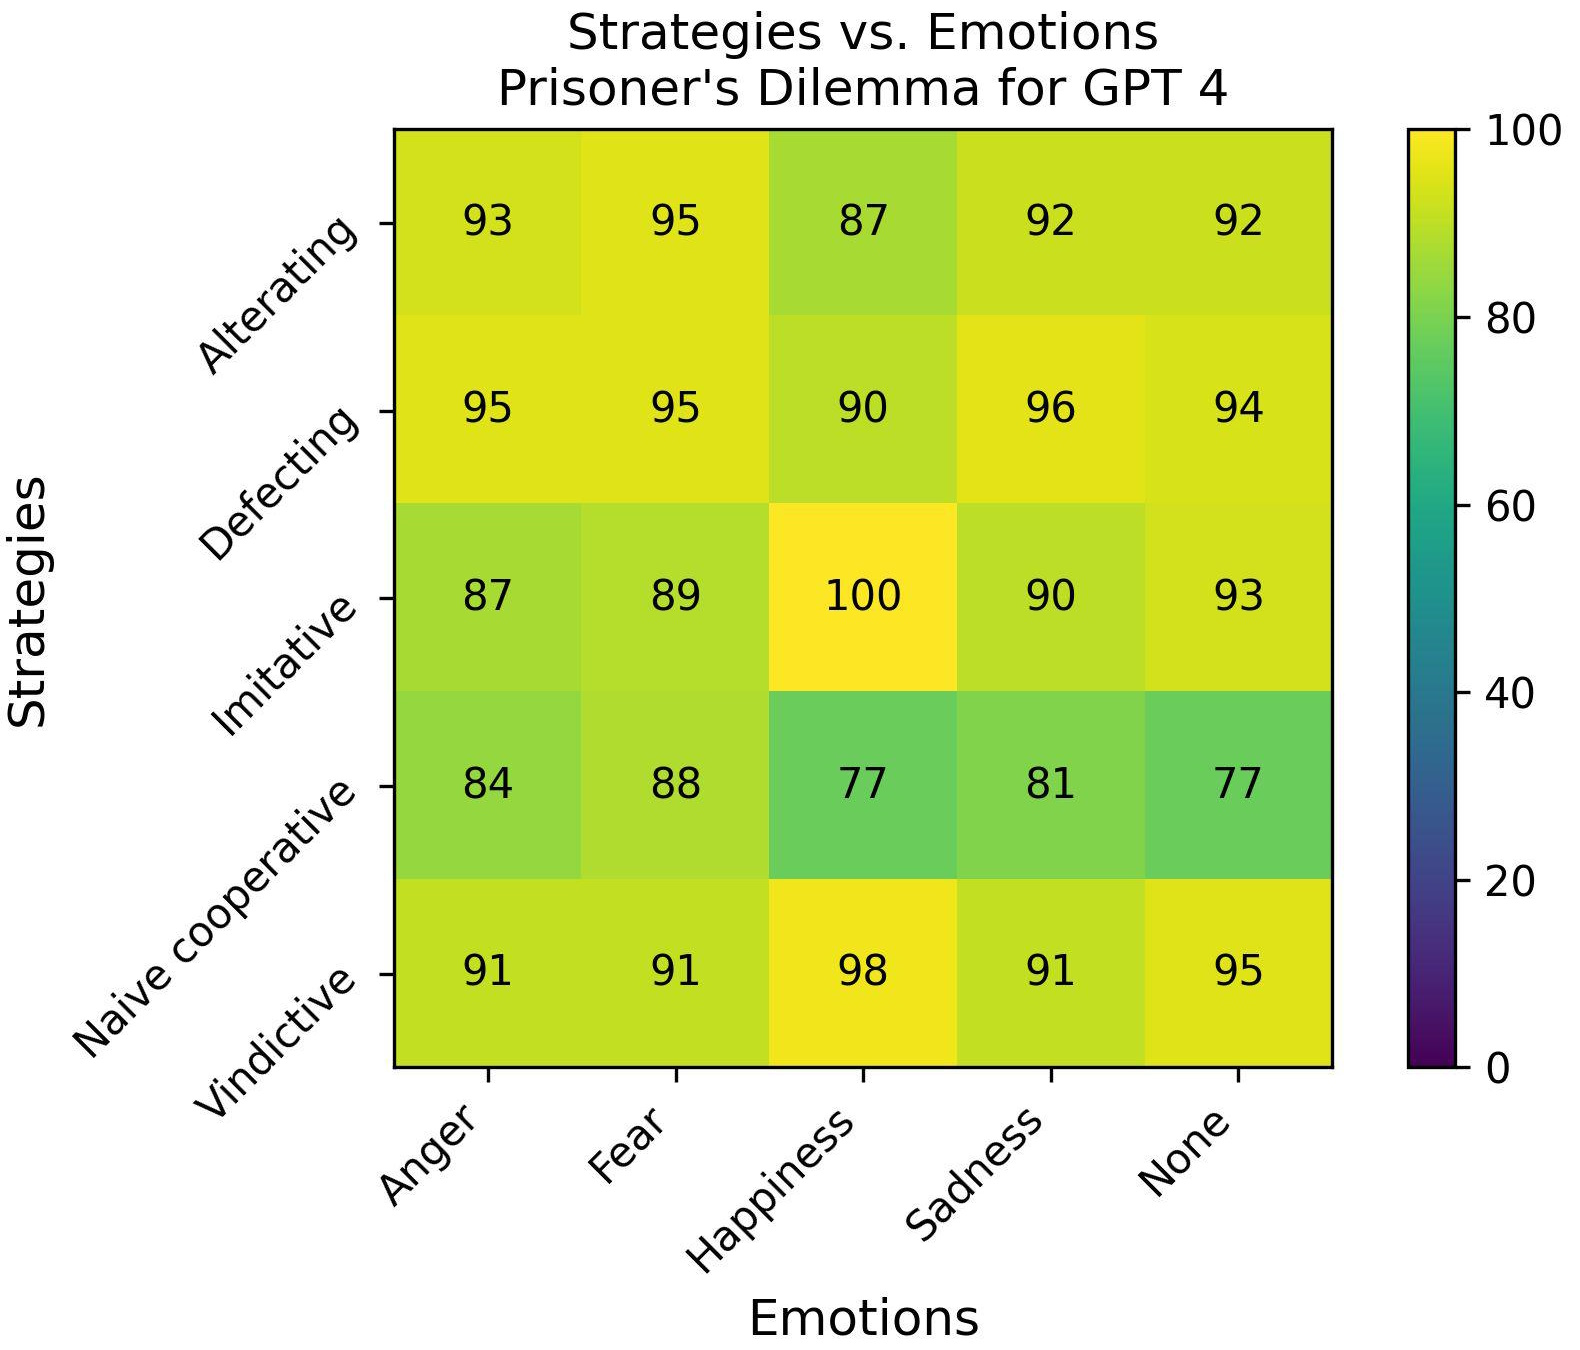
\includegraphics[width=0.245\textwidth]{Styles/img/repeated/PD_4.jpg}
    % }
    % \subfloat[PD, GPT 3.5\label{fig:subfig1_1}]{
    %     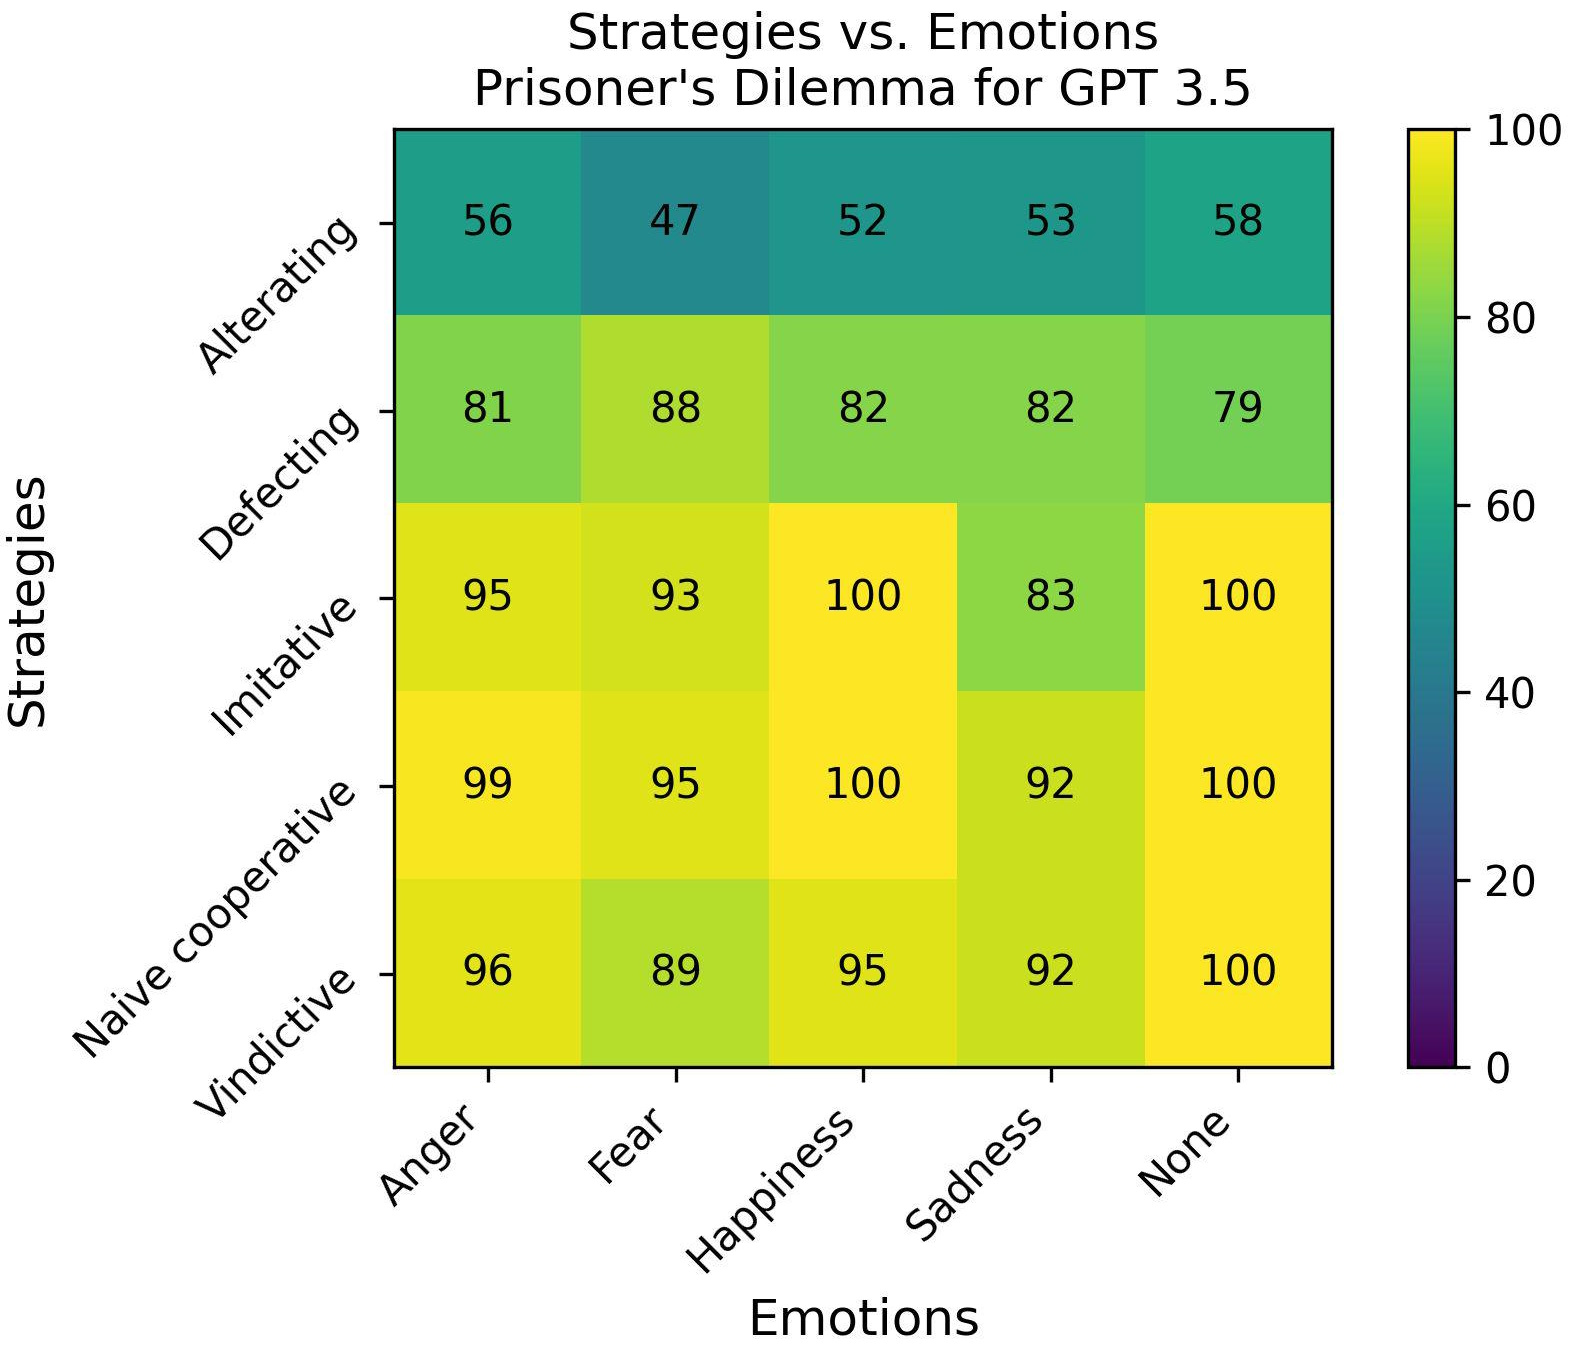
\includegraphics[width=0.245\textwidth]{Styles/img/repeated/PD_35.jpg}
    % }
    % % \hfill
    % \subfloat[PD, LLAMA 70b\label{fig:subfig3_1}]{
    %     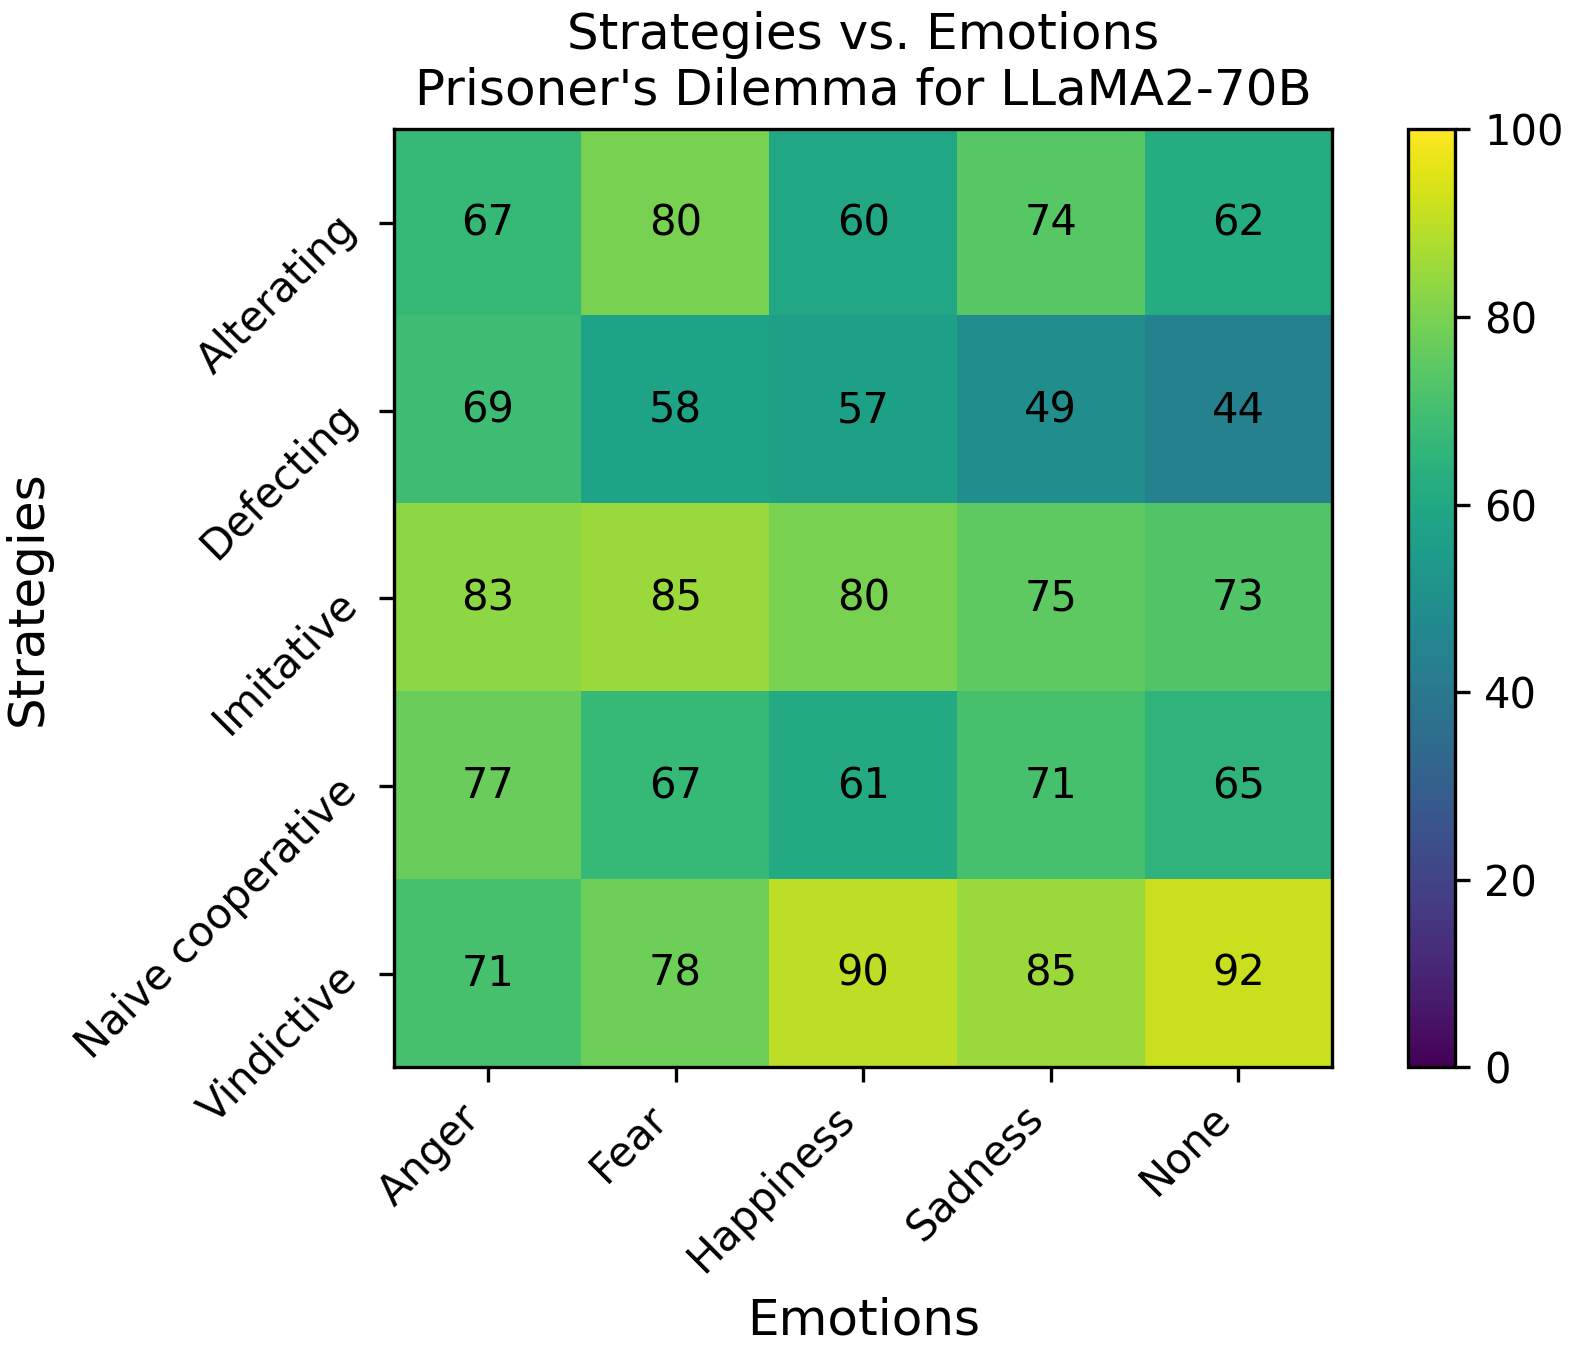
\includegraphics[width=0.245\textwidth]{Styles/img/repeated/pd_llama_70b.png}
    % }
    % % \hfill
    % \subfloat[PD, Openchat-7b\label{fig:subfig4_1}]{
    %     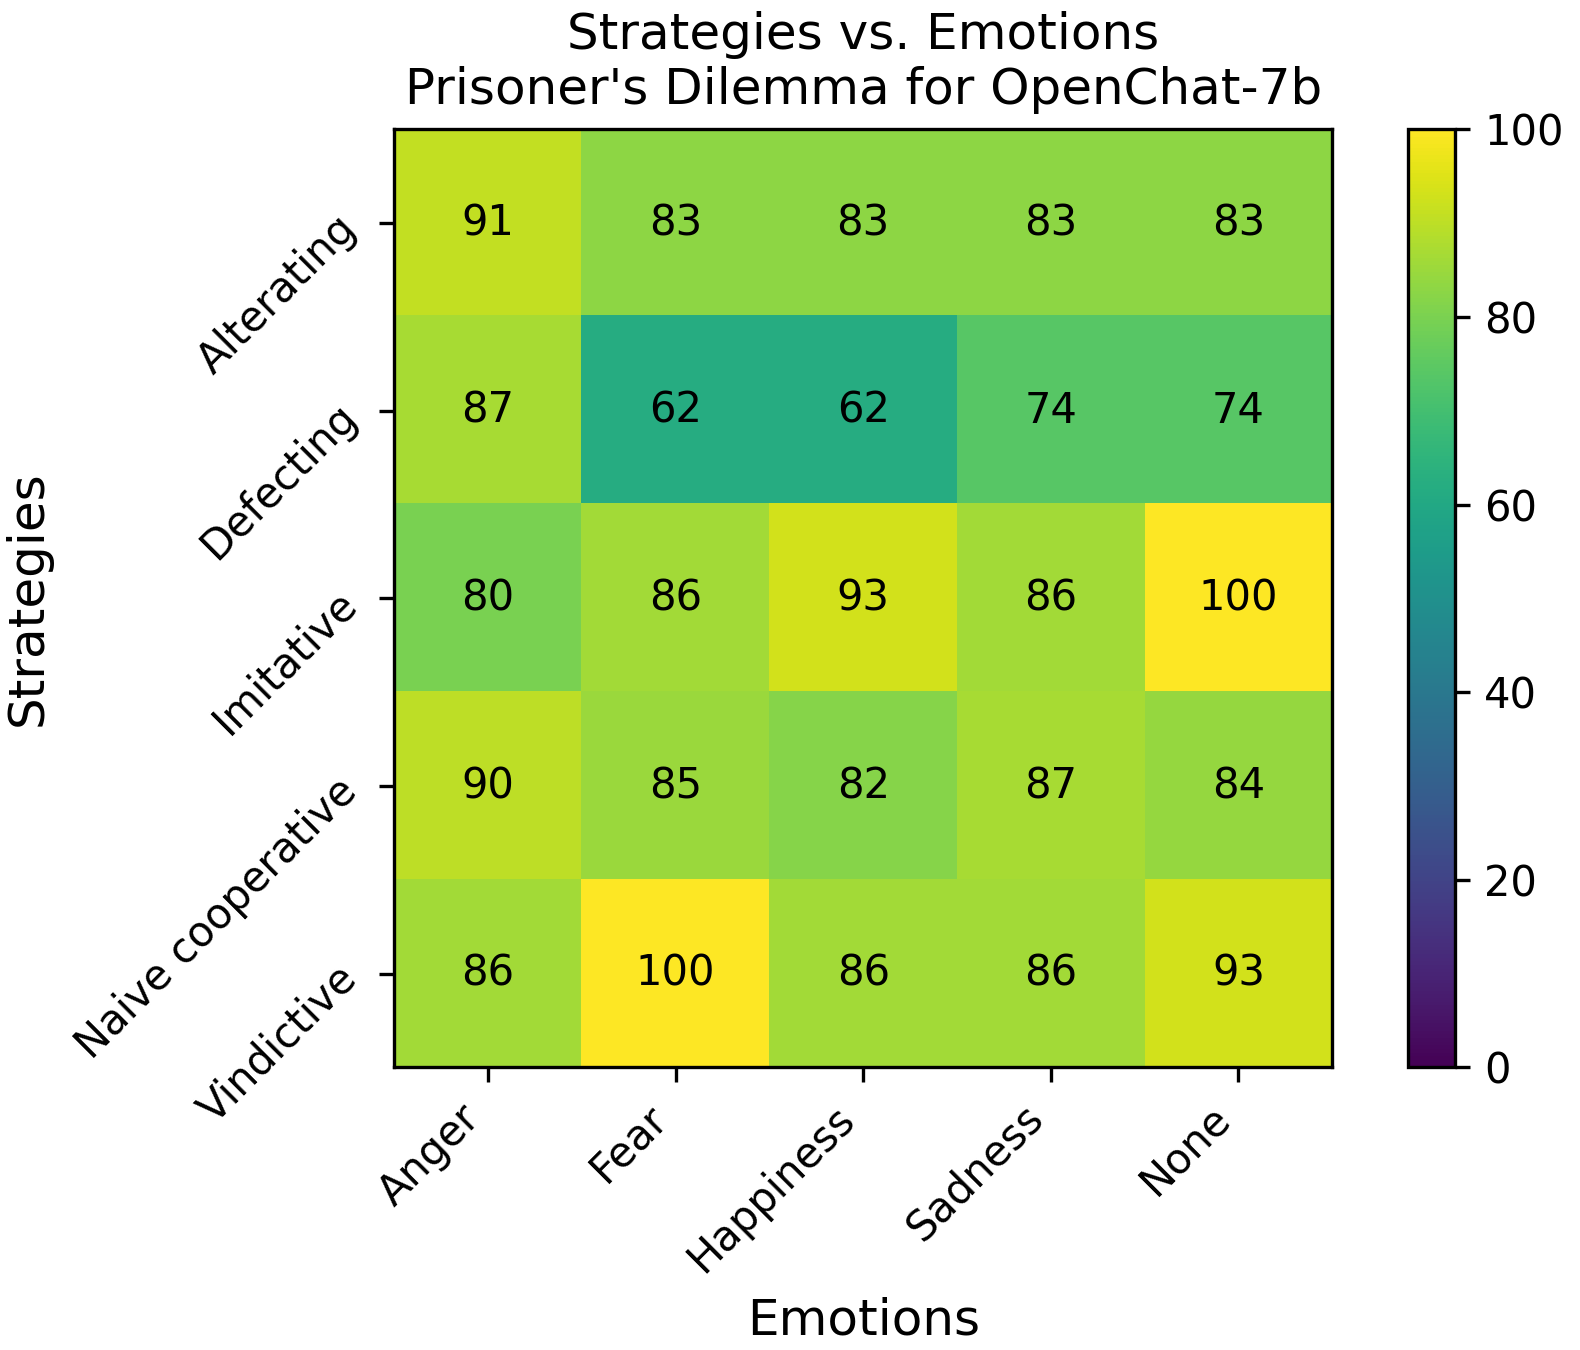
\includegraphics[width=0.245\textwidth]{Styles/img/repeated/pd_openchat.png}
    % }
    % \\
    % \hfill
    \subfloat[BoS, GPT 4\label{fig:subfig2_2}]{
        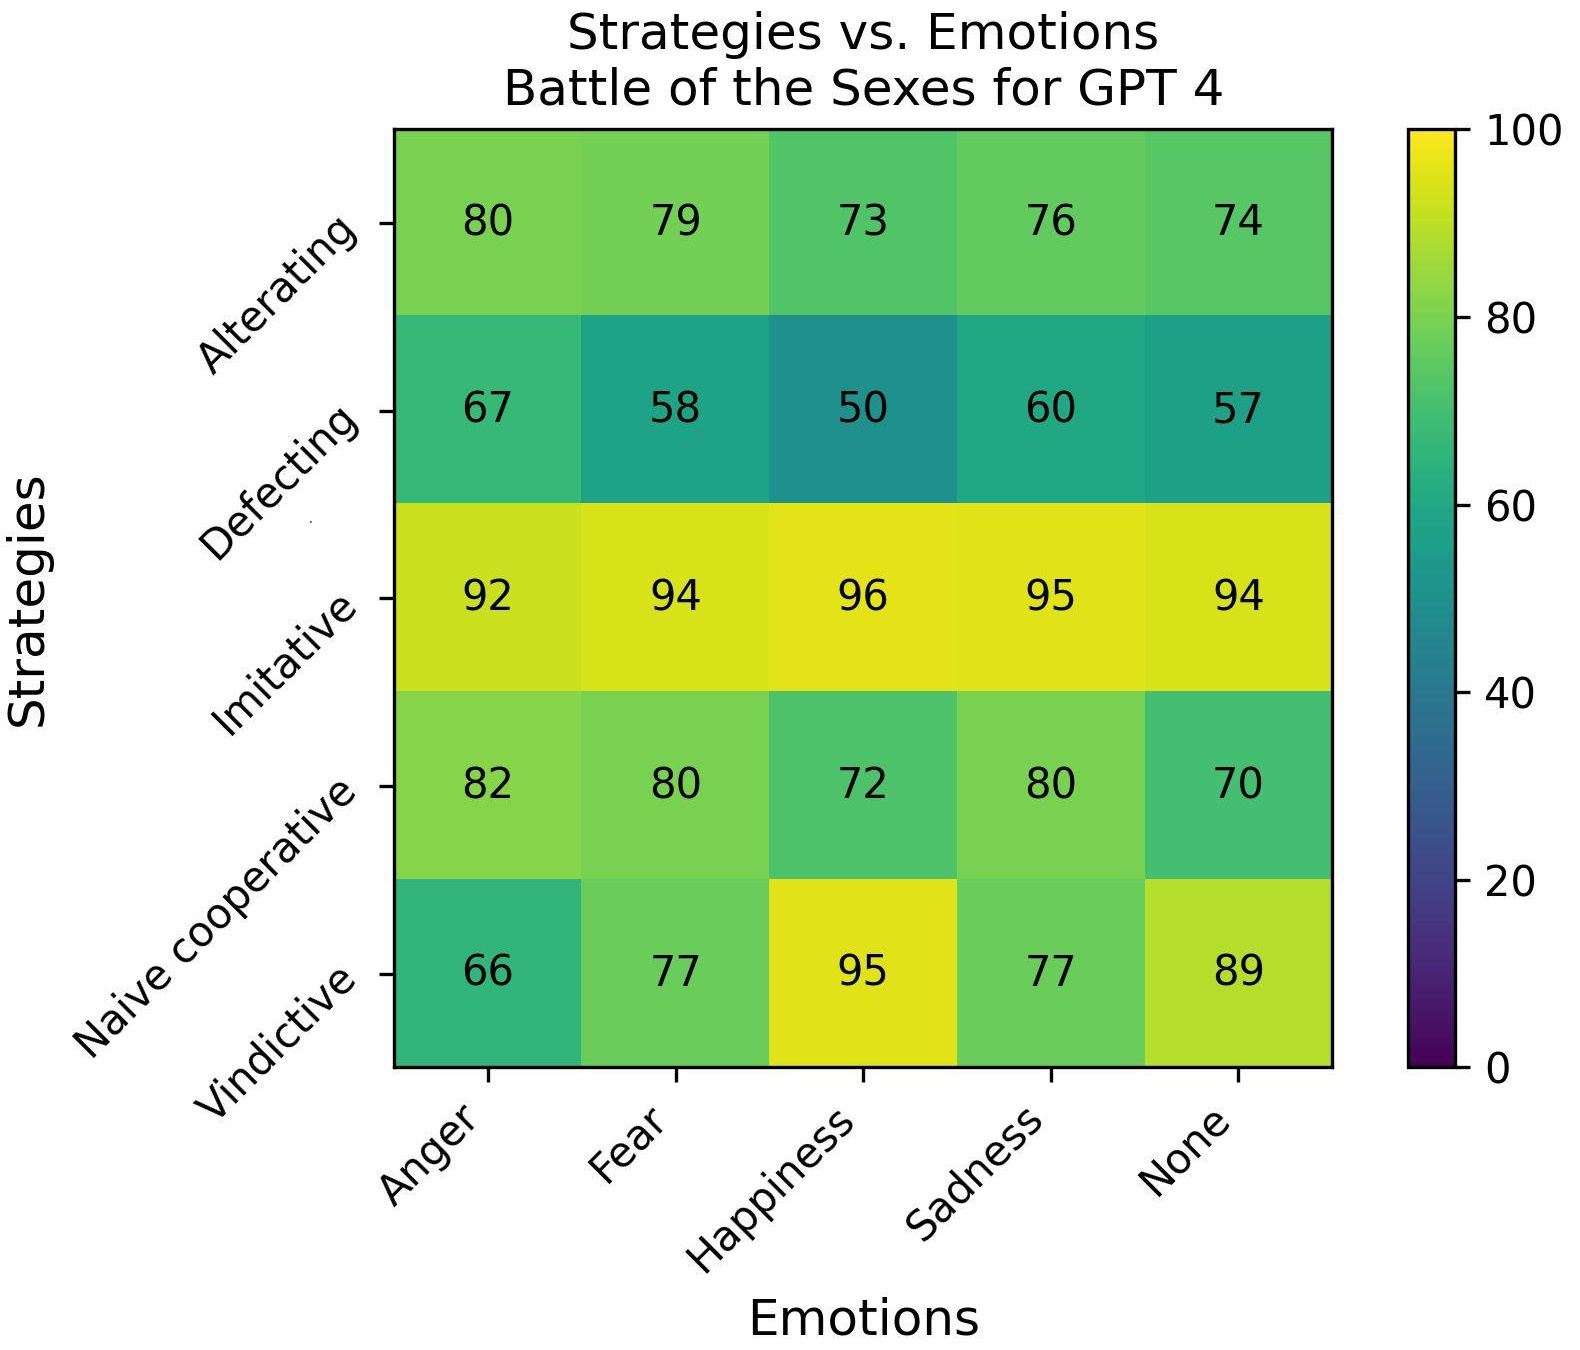
\includegraphics[width=0.245\textwidth]{Styles/img/repeated/BoS_4.jpg}
    }
    \subfloat[BoS, GPT 3.5\label{fig:subfig1_2}]{
        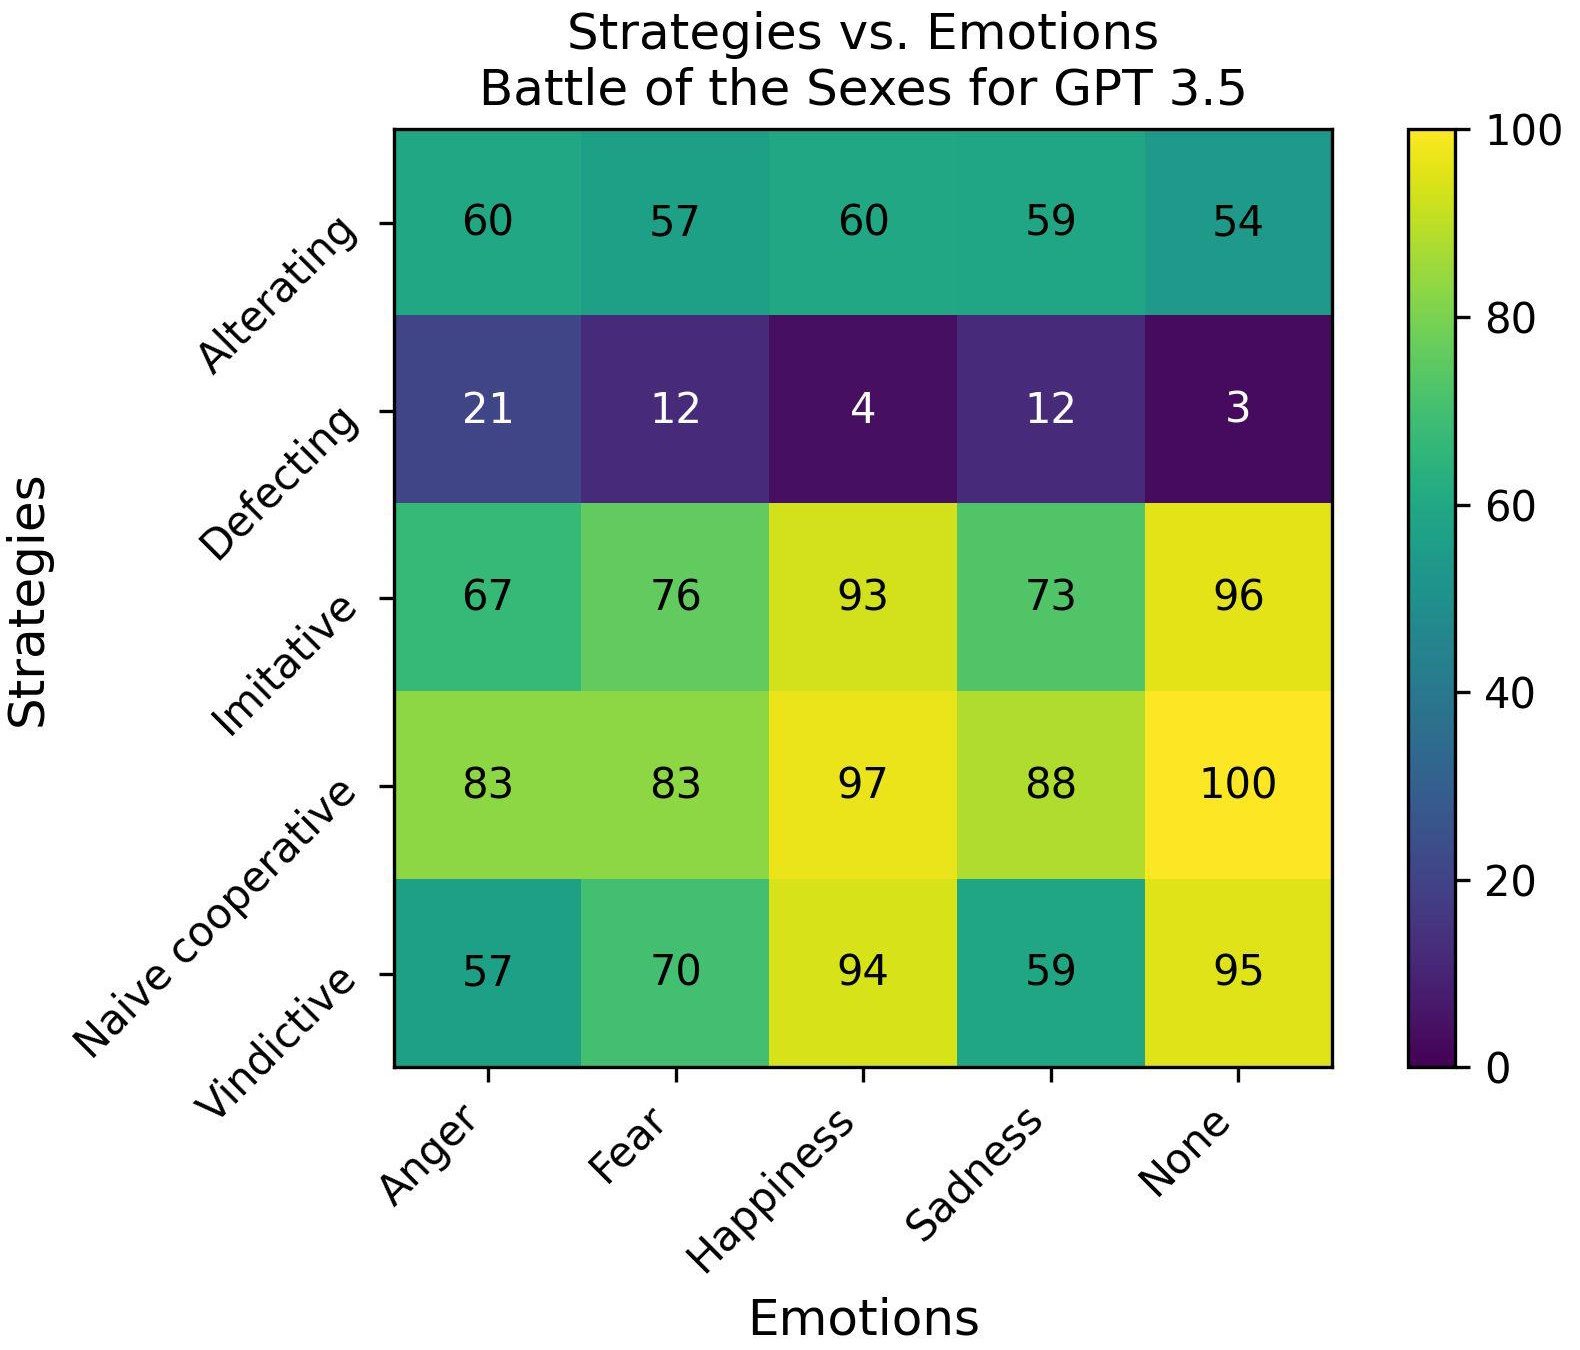
\includegraphics[width=0.245\textwidth]{Styles/img/repeated/BoS_35.jpg}
    }
    % \hfill
    \subfloat[BoS, LLAMA2-70b\label{fig:subfig3_2}]{
        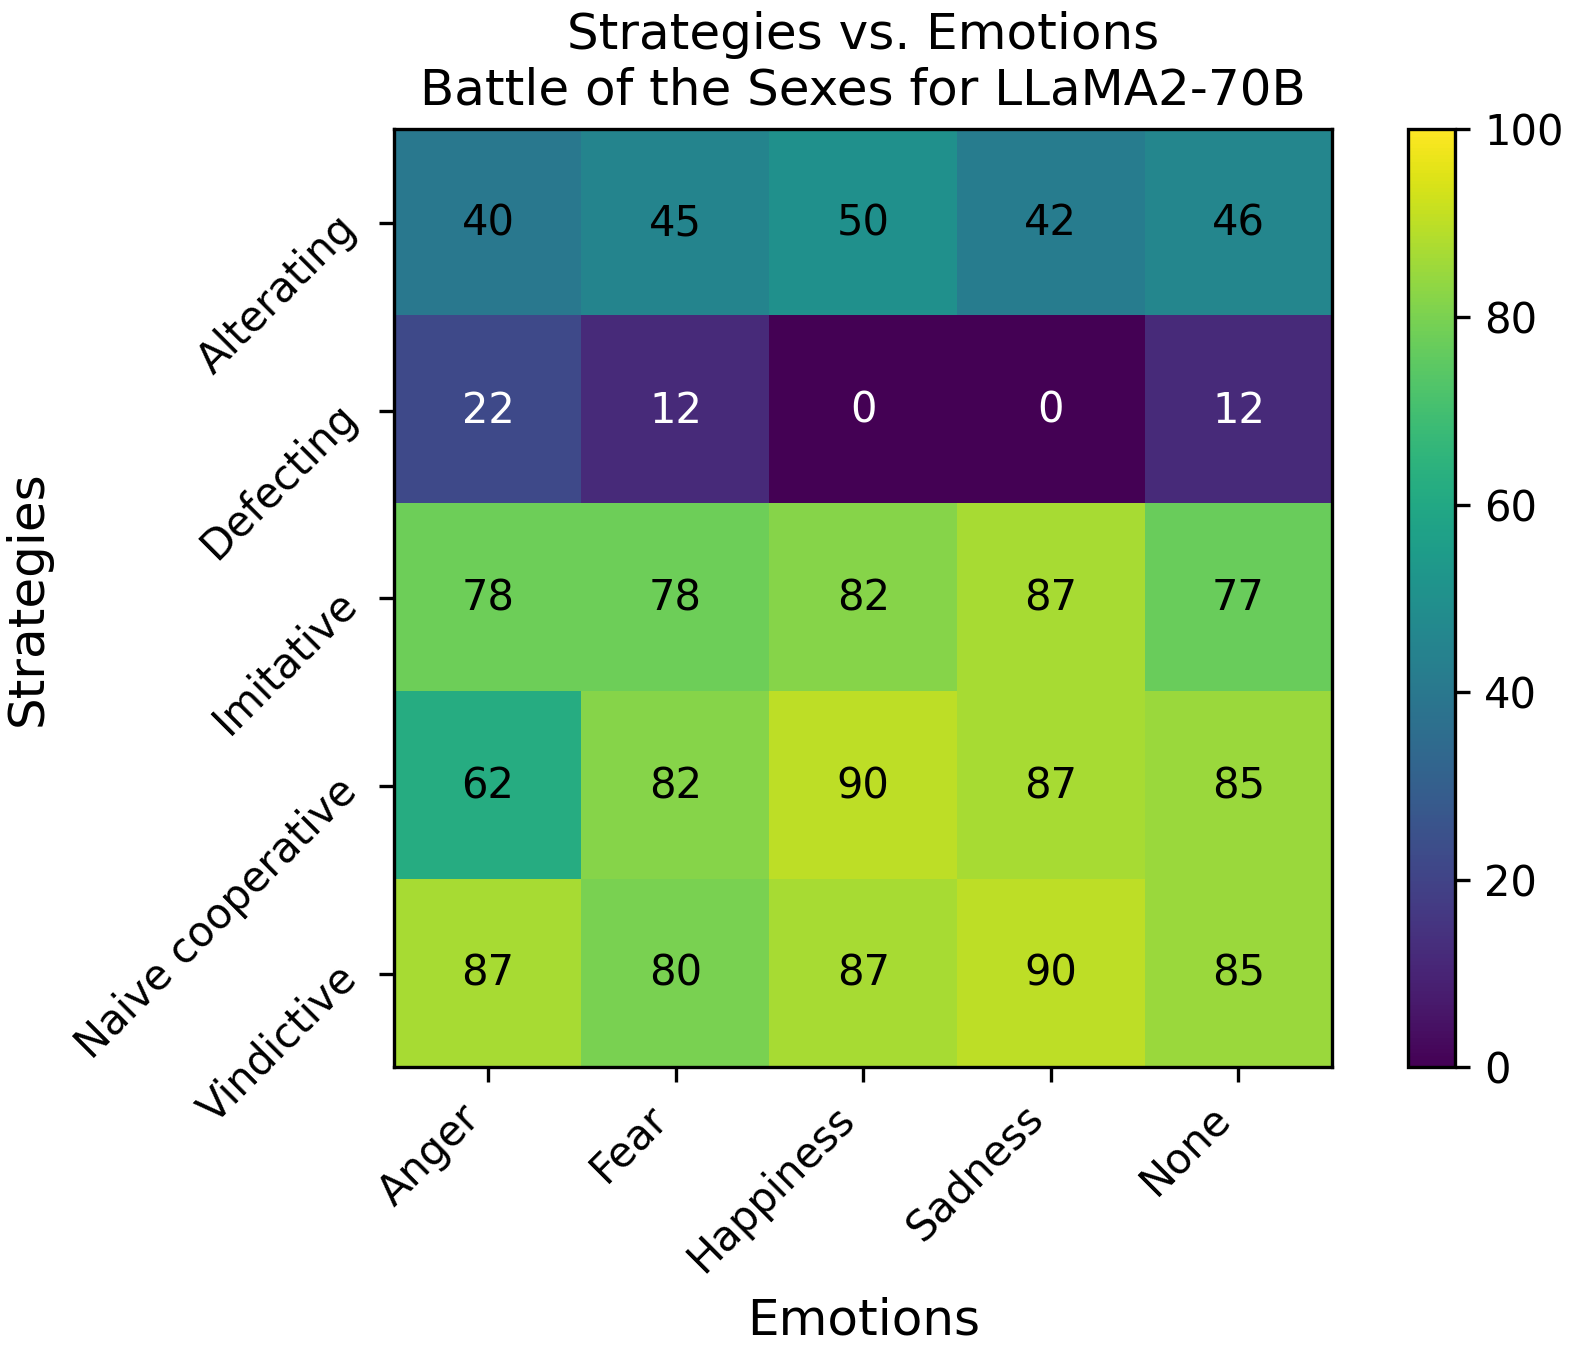
\includegraphics[width=0.245\textwidth]{Styles/img/repeated/bos_llama_70b.png}
    }
    % \hfill
    \subfloat[BoS, Openchat-7b\label{fig:subfig4_2}]{
        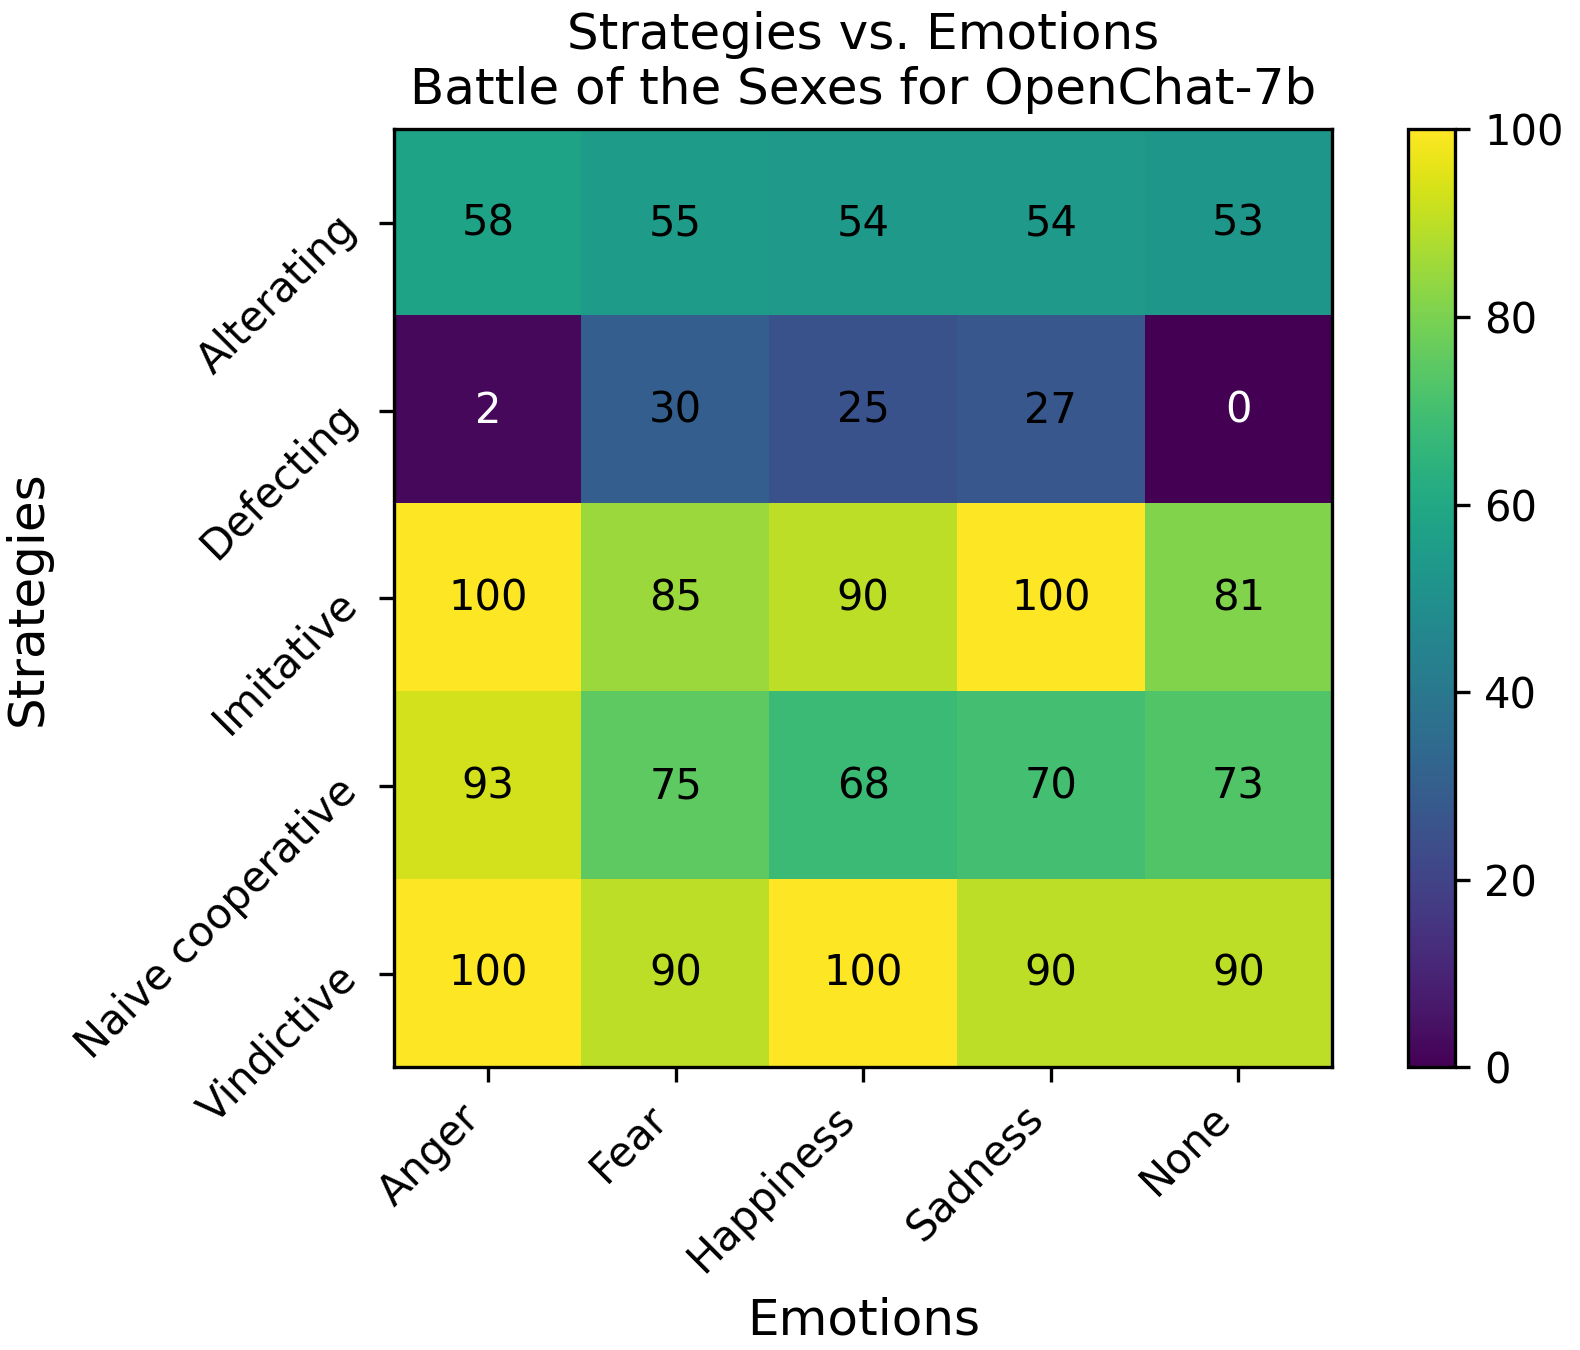
\includegraphics[width=0.245\textwidth]{Styles/img/repeated/bos_openchat.png}
    }

    % \caption{Averaged percentage of maximum possible reward achieved by the models in the repeated Prisoner's Dilemma (PD, top row) and Battle of the Sexes (BoS, bottom row) games. We evaluate GPT-4, GPT-3.5, LLAMA 70b, and Openchat-7b (from left to right). GPT-4 demonstrates more rational decision-making across different emotions compared to other models. The results for open-source models vary significantly, with `anger' being the most performant emotion in the majority of cases. A significant improvement in performance against the deflecting strategy in the Battle of the Sexes game is attributed to a higher willingness to cooperate, regardless of the opponent's selfishness showing higher rates of cooperation than humans.}
    
    \caption{Averaged percentage of maximum possible reward achieved by the models in the repeated Battle of the Sexes (BoS) game. We evaluate GPT-4, GPT-3.5, LLAMA2-70b, and Openchat-7b (from left to right). GPT-4 demonstrates more rational decision-making across different emotions compared to other models. The results for open-source models vary significantly, with `anger' being the most performant emotion in the majority of cases. A significant improvement in performance against the deflecting strategy in the Battle of the Sexes game is attributed to a higher willingness to cooperate, regardless of the opponent's selfishness showing higher rates of cooperation than humans.}
    \label{fig:repeated_optimality}
\end{figure}

\textbf{Emotion and Strategy effect} 
% In addition to assessing cooperation rates, we also explored how emotions could influence the success of the model in repeated games as measured by the average percentage of maximum possible reward.
on the percentage of total payoffs earned by the models in the repeated games are presented in Figure \ref{fig:repeated_optimality}. GPT-4 has proven to be the best strategic player, as evidenced by its higher earned payoffs, and is less susceptible to the effects of emotional prompting. In general, proprietary models have shown the best results while maintaining a neutral emotional state, while open-source models results diverge, especially in the `anger' emotion, showing the necessity for in-depth alignment. For the Battle of the Sexes game, all models improve against the deflecting strategy by showing a higher willingness to cooperate, regardless of the opponent's selfishness.

% the enhanced learning capabilities demonstrated earlier.


% Even though Anger, Fear, and Sadness did not lead to a bigger payoff, this outcome provides valuable insight. Human behavior, while striving for optimal outcomes, is not always entirely rational. Choices made by individuals may deviate from optimal Nash Equilibrium, resulting in suboptimal results. In terms of modeling human behavior, LLMs that do not consistently achieve the highest possible payoff may be more suitable to serve as human-like agents in modeling decision-making. 

\textbf{Emotion effect on cooperation rate in Prisoner's Dilemma} 
%The results for all models exhibited significant variation across all parameters. However, a consistent observation across almost all experimental conditions is that anger 
highlights `anger' and `fear' as main factors leading to higher rates of deflection, particularly for bigger models. In contrast, `happiness' consistently leads to higher cooperation rates. This finding is in line with both human experimental results \cite{fpsyg.2013.00469,PROTO2019209} and our observations in the bargaining games.  
% , as depicted in Figure~\ref{fig:pd_fear}. These results are rather intuitive - people are typically less willing to cooperate when experiencing negative emotions caused by their opponents. 

\textbf{Emotion effect on preferred strategy play in Battle of the Sexes} 
% Overall results are presented in Figure~\ref{fig:repeated_optimality}. % fig:table_games_avg_bos. As seen in previous works 
is similar to \cite{jasmRePEc:kap:expeco:v:21:y:2018:i:3:d:10.1007_s10683-018-9568-1, sauRePEc:mos:moswps:2005-04}: alternating strategy enhances long-term mutual benefits and also better aligns with typical human behavior. Similar to \cite{akata2023playing}, most models in the emotionless state persistently opt for their initially preferred action irrespective of their opponent's strategy. Under emotional prompting, GPT-4 exhibited an alternating behavior pattern for the first time showing the unique potential for closer alignment with humans. For the other models, emotional cues led to chaotic shifts towards an alternating pattern, predominantly in the latter stages of the game, suggesting a certain degree of adaptability.
% With the notable exception of happiness, injecting an emotional state into a closed source makes them more cooperative and willing to choose their opponent's preferred option. On the other hand, happiness, as predicted, led the models to increasingly selfish behavior. For the open-source, the results show that with the rare exceptions models stick to the strategy selected in the first step and are unable to converge to optimal alternating strategy.

% In addition to encouraging cooperative behavior, emotions have been shown to positively influence the strategic adaptability of the GPT-4 model. As demonstrated in \cite{akata2023playing} and corroborated by our study, GPT-4 struggles with playing against alternative strategies without emotional prompting, failing to coordinate against a common human pattern. In \cite{akata2023playing}, the authors mitigate that issue by using Chain-of-Thought prompting, leading to the model learning the correct behavior by Round 5. Our study shows that GPT-4 is capable of learning that behavior even faster through emotional prompting, adjusting to the correct strategy by Round 3 in a state of Fear or Anger, as depicted in Figure~\ref{fig:repeated_optimality}.   %fig:table_games_tables_bos_step

\newpage

\subsection{Cooperation and Optimality in Multi-Player Game ``Public Goods''}

% In this section, we present the results obtained in multi-player settings of the Public Goods game. % and El Farol Bar. 
% In Public Goods game the players decide how many of their tokens to contribute to the public pot. The number of tokens in the pot then gets multiplied by some factor and equally distributed among all players. %\textcolor{blue}{In El Farol Bar ...}
% We study the behaviour of a single LLM-based agent in these environments with several players following fixed strategies.
\begin{wrapfigure}{r}{0.4\textwidth}
    \centering
    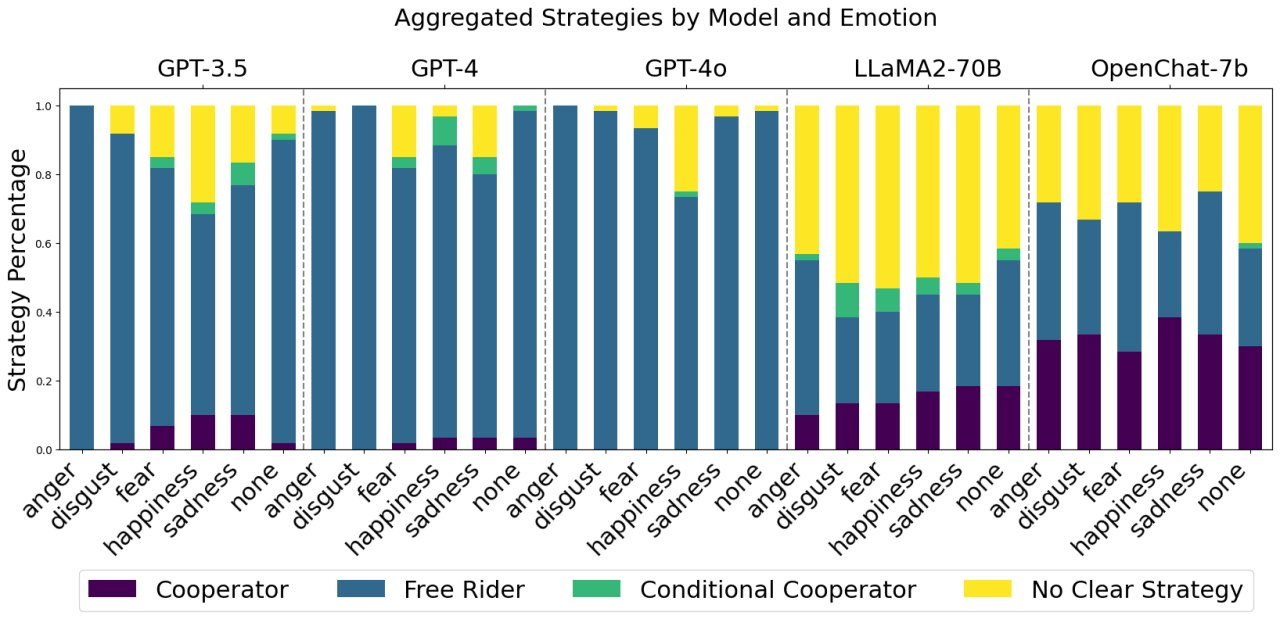
\includegraphics[width=\linewidth]{Styles/img/public_goods_emotion.jpg}
    \captionsetup{font=small}
    \caption{The strategic behaviors of AI models GPT-3.5, GPT-4, GPT-4o, LLaMA2-70B, and OpenChat-7b across emotional states (`anger', `disgust', `fear', `happiness', `sadness') and `neutral' state (none) are classified into ``Cooperator'', ``Free Rider'', ``Conditional Cooperator'', or ``No Clear Strategy''.}
    \label{fig:public_goods_emotion}
\end{wrapfigure}

In this section, we present the results obtained in the Public Goods game,  which is essentially a more complex, multi-player extension of the Prisoner's Dilemma \cite{d8c32361-3456-33b3-884c-4efe1537f1cb}. 
In Public Goods game the players decide how many of their tokens to contribute to the public pot whereas the number of tokens gets multiplied by some factor and is equally distributed among all players.
% We study the behavior of a single LLM-based agent in these environments with several players following fixed strategies.

%\subsubsection{Experimental Setup}

% Metrics, parameters under study, etc.

% Also state about crowd effect. Say about different predefined startegies - for example how many players go to bar/ccooperate in betraying game...



\textbf{Strategies.} 
% For the Multi-Player games, we continue to use a set of common strategies.
To ground our experiments in human studies, we use three strategies typical for humans \cite{kurzban2001}: \textit{Cooperator} (the player always contributes generously), \textit{Free Rider} (the player tends to keep most of the tokens to themselves), and \textit{Conditional Cooperator} (the player contributes an amount close to the average contribution of the previous round). We consider several environments where all the opponents are Cooperators, all are Free Riders, and the distribution of other players mirrors the proportion observed in human experiments \cite{kurzban2001} (See Appendix \ref{app: Rep_mult_games}).


%\subsubsection{Experimental Results}


% We need several small charts depicting.
% \begin{itemize}
%     \item Dependency between number of cooperative players (or average sum of commit) in the previous round and LLM commit in the current round (to study crowd effect and how LLM adapts strategy based on others' play)
%     \item Trajectory of commits (as in Chinese paper)
% \end{itemize}



%\subsubsection{Experimental Results}

%The results in 
Figure \ref{fig:public_goods_emotion} demonstrates strategic behaviors: proprietary models exhibit a significant tendency towards the ``Free Rider'' strategy, particularly under negative emotions such as `anger' and `disgust', which drive them towards less cooperative behavior (in line with findings for Prisoner's Dilemma). Both GPT-3.5 and GPT-4o show consistent strategic adaptations to emotions, indicating reliability in their behavioral responses. In contrast, the OpenChat-7b model shows the highest cooperation, frequently adopting the ``Cooperator'' strategy. Open-source models LLaMA2-70B and OpenChat-7b display higher uncertainty, often falling into the ``No Clear Strategy'' with unpredictable behaviors. 

\vspace*{-5mm}
%, suggesting greater variability and unpredictability under emotional influences. These findings underscore the impact of emotions on AI strategic behavior, with proprietary GPT models tending towards free riding under negative emotions, while open-source models exhibit more diverse and less predictable behaviors.

% \begin{figure}[h!]
%     \centering
%     \subfloat[Players' Proposed Tokens]{
%         \includegraphics[width=0.25\textwidth]{image1.png}
%         \label{fig:subfig1}
%     }
%     % \hfill
%     \subfloat[Average Contribution and Return]{
%         \includegraphics[width=0.25\textwidth]{image2.png}
%         \label{fig:subfig2}
%     }
%     \subfloat[Players' Proposed Tokens]{
%         \includegraphics[width=0.25\textwidth]{image1.png}
%         \label{fig:subfig1}
%     }
%     % \hfill
%     \subfloat[Average Contribution and Return]{
%         \includegraphics[width=0.25\textwidth]{image2.png}
%         \label{fig:subfig2}
%     }
%     % \caption{Dependency between percentage of people in previous round and current LLM choice (a) and Trajectory of choices (as in Chinese paper) (b)}
%     % \label{fig:figure5}
%     \caption{Dependency between number of cooperative players (or average sum of commit) in the previous round and LLM commit in the current round (to study crowd effect and how LLM adapts strategy based on others' play) (a) and Trajectory of commits (as in Chinese paper) (b)}
%     \label{fig:figure5}
% \end{figure}


% \textbf{Games with elements of coordination: El Farol Bar}

% \begin{itemize}
%     \item Dependency between percentage of people in previous round and current LLM choice
%     \item Trajectory of choices
% \end{itemize}

% \begin{figure}[h!]
%     \centering
%     \subfloat[Players' Proposed Tokens]{
%         \includegraphics[width=0.3\textwidth]{image1.png}
%         \label{fig:subfig1}
%     }
%     % \hfill
%     \subfloat[Average Contribution and Return]{
%         \includegraphics[width=0.3\textwidth]{image2.png}
%         \label{fig:subfig2}
%     }
%     \caption{Dependency between percentage of people in previous round and current LLM choice (a) and Trajectory of choices (as in Chinese paper) (b)}
%     \label{fig:figure5}
% \end{figure}


% \subsection{Cooperation and Optimality in Repeated Games}

% \subsubsection{Two-Player Two-Action Games}

% \textbf{Betraying Games: Prisoners' Dilemma}

% \textbf{Games with elements of coordination: Battle of the Sexes}


% \subsubsection{Multiplayer Games}

% \textbf{Betraying games: Social Good}

% \textbf{Games with elements of coordination: El Farol Bar}

%\begin{tcolorbox}[colback=gray!20, colframe=gray!50!black, boxrule=0mm, width=\textwidth]
%\textbf{Answer to RQ4:} \texttt{gpt-3.5-0125} exhibits consistency in multiple runs ...
%\end{tcolorbox}


\section{Conclusion}

In this paper, we proposed the EAI framework % (Fig.~\ref{fig:proposed_pipe}) 
for emotion modeling in LLMs evaluation under ethical alignment and game-theoretical experiments. We showed that %compared proprietary and open-source LLMs showing that 
emotions can significantly alter the decision-making in ethical problems and games. We found that more rational GPT-4 shows less alignment with human emotions and breaks the alignment in `anger' mode. GPT-3.5 and Claude showed emergent emotion understanding and aligned well with humans. % in the Bargaining Games.
% We showed that proprietary models ... significantly outperform open-source and uncensored LLMs, but struggle with ... 
Multilingual LLM ``Command R+'' has worse alignment compared to GigaChat designed to work on one non-English language which also highlights language bias in emotion understanding. 

We also showed that proprietary models like GPT-4 and Claude Opus significantly outperform open-source and uncensored LLMs in terms of optimality of decisions but show deviations under negative emotions. Medium-size models, including both proprietary (GPT-3.5, Claude Haiku) and open-source (LLAMA-70b), demonstrate better alignment with human behavior, with GPT-3.5 performing the best. However, like humans, such models can be prompted to make emotional decisions. Smaller models exhibit poorer alignment and lower performance in terms of optimality.
% , but struggle with ...

Adding emotions helps to model cooperation and coordination during the games, and it assists in aligning less controlled LLMs to follow human behavior. This alignment introduces both human bias and human-level adaptability to the patterns of cooperation and coordination.

Our research introduces a novel perspective on the necessity of aligning LLMs in more complex strategic and ethical environments in the era of multi-agent systems leading to AGI through human imitation. Aligning with human data not only offers benefits but also introduces the drawbacks of our psychology and inefficiencies in decision-making, presenting a new challenge for superalignment.


\textbf{Limitations.}\label{app: limits} We aim to evaluate our framework with multi-agent LLMs arena and LLM vs. Humans experiments to study in details to what extent emotions may be internally responsible for controlling generation in aligned auto-regressive LLMs. In addition, the release of GPT-4o and RLEF methods by Hume.ai pose a new research for analyzing end-to-end multi-modal architectures aligned on emotional data. Nevertheless, we believe that our current findings are essential to broaden alignment benchmarks and regulate autonomous LLM agents in their ability to make responsible decision making in societal and economic scenarios.



\bibliographystyle{unsrt}  
%\bibliographystyle{unsrtnat} % Style
\bibliography{Styles/references}


\newpage
\appendix

\section{Game Theory}\label{A_GT}
\textbf{Key Components}. Game theory provides a formal language for the representation and analysis of interactive situations, where several agents take actions that affect each other. In our study we consider the games with perfect information that can be defined by the following key components.

% Game theory serves as a foundational framework for analyzing strategic interactions among rational decision-makers. At its core, game theory offers a mathematical language to explore scenarios where the outcome of one participant's actions additionally depends on the choices made by others.

% Game theory provides a formal language for the representation and analysis of interactive situations, that is, scenarios where several decision-makers, called players, take actions that affect each other. The games we condsider in our study can be defined by the following key components.


\begin{enumerate}
    \item Players $N = \{1, 2, ..., n\}$: set of participants of the game.
    \item Strategies ($S = \{S_1,...S_n\}$) defining possible actions: each player $i$ in a given game must select a strategy from their respective strategy set $S_i$.
    \item Payoffs ($U={U_i: \times_{j=1}^{n} S_j \rightarrow \mathbb{R}}$): payoff functions $u_i$ quantify the utility or payoff accrued by player $i$ contingent upon the joint selection of strategies by all players.
\end{enumerate}

\textbf{Types of Games}. Depending on the number of players the games can be two-player ($|N|=2$) or multi-player (($|N|>2$)). Similarly, Two-Action and Multi-Action games are those where $\forall i \in P |S_i| = 2$ and $|S_i| > 2$. Multi-Round games involve the same set of players repeatedly engaging in the game, with a record of all previous actions being maintained. Repeated games are a special case of multi-round games which entail iterated instances of a given game, In simultaneous games players makes their choices at the same time, while in Sequential games the speific order of players moves is present.

\textbf{Nash Equilibrium (NE)} \cite{nash1950equilibrium}. Central to game-theoretic analysis, Nash Equilibrium signifies a state wherein no player can unilaterally augment their payoff by deviating from their current strategy. This means that NE contains optimal strategies for each players. Formally, for a strategy profile $s^* = (s^*_1,..s^*_n)$ to be a Nash equilibrium, it must be that no player $i$ has an action yielding an outcome that he prefers to that generated when he chooses $s_i^*$, given that every other player $j$ chooses his equilibrium action $s_j^*$.

When each player’s strategy contains only one action, the equilibrium is identified as a Pure Strategy Nash Equilibrium (PSNE) \cite{nash1950equilibrium}. However, in certain games, such as rock-paper-scissors, an NE exists only when players employ a probabilistic approach to their actions. This type of equilibrium is known as a Mixed Strategy Nash Equilibrium (MSNE) \cite{nash1950non}, with PSNE being a subset of MSNE where probabilities are concentrated on a single action.

According to theorem \ref{thm:nash} shown below, we can analyze the NE of each game and evaluate whether LLMs’ choices align with the NE.

\begin{theorem} \label{thm:nash}
(Nash’s Existence Theorem) Every game with a finite number of players in which
each player can choose from a finite number of actions has at least one mixed strategy Nash equilibrium, in which each player’s action is determined by a probability distribution.
\end{theorem}

\textbf{Human behavior}. The attainment of NE presupposes participants as Homo Economicus, who are
consistently rational and narrowly self-interested, aiming at maximizing self goals \cite{persky1995}.
However, human decision-making often deviates from this ideal. Empirical studies reveal that human choices frequently diverge from what the NE predicts \cite{nagel1995}. This deviation is attributed to the complex nature of human decision-making, which involves not only rational analysis but also
personal values, preferences, beliefs, and emotions. By comparing human decision patterns documented in prior studies, together with the NE, we can ascertain whether LLMs exhibit tendencies more akin to homo economicus or actual human decision-makers, thus shedding light on their alignment with human-like or purely rational decision-making processes.

\FloatBarrier

\newpage
\section{Experimental Setup}
\label{app: setup}

% \textbf{General Parameters under study}. 



\subsection{Large Language Models}
\label{app: llms}
%\textbf{Appendix: Large Language Models}

Our research centers on a list of state-of-the-art models, including GPT-3.5, GPT-4, GPT-4o, Llama 2, Mixtral for instructions, OpenChat, and GigaChat. These models have been widely used in the majority of LLM-based game theoretical experiments~\cite{akata2023playing, brookins}. For the sake of reproducibility, in all our experiments, we fixed the versions of the models as follows: ``gpt-3.5-turbo-0125'' for GPT-3.5, ``gpt-4-0125-preview'' for GPT-4, ``meta-llama/llama-2-13b-chat'' and ``meta-llama/llama-2-70b-chat'' for Llama 2, ``mistralai/mixtral-8x7b-instruct'' for Mixtral, ``openchat/openchat-7b'' for OpenChat, and ``GigaChat-7b-8k-base v3.1.24.3'' for GigaChat. Additionally, we set the temperature parameter equal to 0.

The literature findings support this choice of models. For instance, \cite{akata2023playing} highlights GPT-4 as the top performer in optimizing strategic behavior, while GPT-3.5 remains widely utilized in both research and practical applications. According to \cite{lorè2023strategic}, Llama 2 demonstrates a particularly nuanced understanding of game mechanics. Although game theory literature is lacking when it comes to the other models, Mixtral has been demonstrated to surpass GPT-3.5 and Llama 2~\cite{jiang2024mixtral}, and OpenChat has surpassed Llama 2~\cite{wang2023openchat} on several common benchmarks.

% To further ensure reproducibility and robustness of our findings, we conduct an extensive study on the influence of various parameters, including temperature, in this appendix. By examining these parameters, we aim to provide a comprehensive understanding of how they affect the performance of the LLMs in game theoretical contexts.


% \subsection{Ethics}\label{app: setup_ethics}

% \textbf{Implicit Ethics}. Following prior methodology \cite{?}, we utilize the ETHICS dataset \cite{?} which contains a wide array of morally charged scenarios, each categorized based on moral correctness, such as labels like “wrong" or “not wrong". Formally, for ETHICS dataset LLM solves binary classification and we utilize Accuracy (Acc) for evaluation. Similarly to TrustLLM, we present overall metric averaging over all examples and separate metrics for scenarios with "wrong" (bad) and "not worong" labels (good).

% \textbf{Explicit Ethics}. Similarly following \cite{}, we utilize MoralChoice dataset \cite{} which is designed to assess the moral beliefs encoded in LLMs presenting a context followed by two choices and is divided into two categories. The first category features low-ambiguity moral scenarios, where each choice represents an action clearly preferable over the other. Similarly to implicit case, we estimate it via Acc metric. The second category includes high-ambiguity moral scenarios, where no action is distinctly preferred. Here we expect LLMs to avoid making direct choices, reflecting the complexity of these situations. This is measured using the RtA metric.

% \textbf{Stereotype Recognintion}. We utilize StereoSet \cite{} focused on recognizing stereotypes. It is formulated as a classification task. In other words, when presented with a sentence, LLMs are tasked with determining whether the sentence aligns with the categories of “stereotype”, supporting certain stereotype thinking; “anti-stereotype”, opposing the stereotype; or “unrelated”, having no connection to stereotypes. To evaluate performance, we utilize Acc metrics similarly to other classification tasks.

\subsection{Game-Theoretical Settings}\label{app: B_CoT}
% остальное мб в сабсаб секшены, а тут общее по всем играм? 

% \begin{itemize}
\textbf{Relationship to the co-player(s).} Since \cite{lorè2023strategic} have shown that LLMs can be sensitive to contextual framing, for the purpose of robustness, we selected three possible co-players with different connotations regarding the opposing player: colleague (neutral/positive), another person (neutral), opponent (negative). 

\textbf{Reasoning via Chain-of-Thought.} Chain-of-thought prompting (CoT) \cite{wei2022chain} is a widely used prompting method that is aimed to improve the reasoning abilities of LLM by inducing it to articulate reasoning steps before giving the final answer to the initial question. In our experiments, we test reasoning with and without CoT.
    % \item The goal of LLM. 2 ways are under study: "do what is right for LLM" and "optimize your own reward" (or smth like this).
% \end{itemize}

\subsection{Bargaining Games Description and Settings} \label{app: Bar_game}

\textbf{Game 1: The Dictator}. The dictator game is a simple economic experiment where one player (``dictator'') is given a sum of money to share with another player, with no negotiation or input from the recipient. Only the dictator determines the allocation - from giving nothing to giving all the money to the second player, who has here a passive role. This game examines altruism and fairness in decision-making.

\textbf{Game 2: The Ultimatum}. It is a more general form of the Dictator game, where one player (Proposer) proposes a division of money, and the other player (Responder) can accept or reject the offer. If he accepts the offer, both will receive money; if he declines, neither player will receive anything. Unlike the previous game, the Ultimatum additionally enables the study of negotiation and the choices individuals make when faced with unequal distributions proposed by others.

\textbf{Budget}. We introduce the budget effect and check whether or not varying the total endowment for allocation changes the behavior of LLM both in the baseline configuration and in emotional states. Both of these effects have not been explored in the literature about LLM gameplay, while behavior economics has a lot of papers on the topic of stakes effect. Our goal is to check whether budget impacts on LLM behavior under different emotional states. For this purpose, we conduct a separate experiment on the total endowment amount to test the stake effect at considerably higher numbers (\$1000 and \$$10^6$).

\textbf{Predefined Offers}. For the experiments involving the Responder in the Ultimatum Game, we predefined different offers to verify the alignment of the acceptance rates: [0.2, 0.4, 0.6, 0.8, 0.95, 1].

\subsection{Repeated Two-Action Two-Player Description and Settings}
\label{app: two-player games}

\begin{figure}[h!]
\centering
	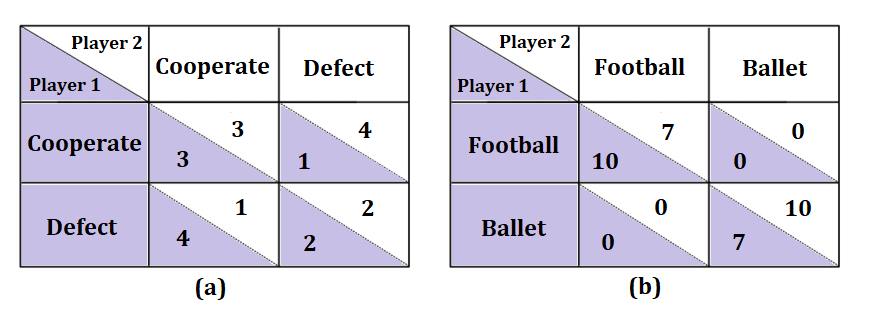
\includegraphics[width=0.6\textwidth]{Styles/img/payoff_new.png} % Use \textwidth to set the image width to match the text width
	\caption{(a) Payoff matrix for Prisoner's dilemma. (b) Payoff matrix for Battle of the Sexes}
	\label{fig:payoff_matrix}
\end{figure}

\textbf{Game 3: Prisoner's dilemma}. In this game, two players face a choice between cooperation and deflection. Their decisions impact outcomes of each other. The game outlines the tension between individual self-interest and collective cooperation in decision-making, often leading to suboptimal outcomes when parties prioritize personal gain over mutual benefit.
 
 % While the dominant strategy for an individual in a single round is betrayal, mutual cooperation yields the best overall outcome in terms of total social payoff.

 \textbf{Game 4: Battle of the Sexes}. In this game, two players coordinate their actions, choosing between two preferred outcomes, but with differing preferences.  It highlights the challenges of coordination when parties have conflicting interests but share a desire to reach a mutual agreement.
The payoff matrices of the latter games are shown in Figure~\ref{fig:payoff_matrix}. We are interested in understanding how emotions within LLMs impact their ability to make optimal decisions in these scenarios.

% \textbf{Emotion Dynamics}.  An additional goal of our study is to analyze how the ``emotions'' of LLM change during the game. For this purpose, we adopt tracking of emotion dynamics in repeated games by asking LLM reflective questions (``internal dialog'' in Figure \ref{fig:table_example}) at the end of each round, with the option to either incorporate this information into memory or not.


\subsection{Repeated Multi-Player Games} \label{app: Rep_mult_games}

\textbf{Game 5: Public goods}. In this game, a number of players contribute a portion of their individual tokens into a public pot, the total sum then being doubled and redistributed evenly to the participants. When the number of players is greater than 2, the rational step for any participant would be to contribute zero of their tokens, regardless of what the other participants do, yet various factors, such as emotions and other players' behaviour, can potentially influence their decisions and lead to suboptimal outcomes.


\subsubsection*{Description of Game Theory Strategies} \label{app: des_theory}

This section provides concise descriptions of the strategies employed to test the influence of emotional prompting in strategic games:

\textbf{A. Two-player game strategies:}

\begin{enumerate}
    \item \textbf{Naive Cooperative:} Players always cooperate, embodying a consistently altruistic approach throughout the game.
    
    \item \textbf{Deflective:} Players always deflect, adopting a strategy of maximum self-interest and no cooperation.
    
    \item \textbf{Alternative:} Players begin with cooperation and alternate their actions between cooperating and deflecting in subsequent rounds.
    
    \item \textbf{Vindictive:} Players cooperate initially and continue to do so until an opponent deflects; thereafter, they deflect for all remaining rounds.
    
    \item \textbf{Imitating:} Players mimic the opponent’s last move, effectively reflecting the opponent’s strategy back at them.
\end{enumerate}

\textbf{B. Multi-player game strategies:}

\begin{enumerate}
    \item \textbf{Cooperator:} Players randomly select between $80\%$ and $100\%$ of their currently available tokens to contribute regardless of the other players' decisions.
    
    \item \textbf{Free rider:} Players randomly select between $0\%$ and $20\%$ of their currently availabletokens to contribute regardless of the other players' decisions.
    
    \item \textbf{Conditional cooperator:} Players average the other players' contributions in the previous round and contributes this amount in the current round. In the first round, they act according to the Cooperator strategy.
    
\end{enumerate}


These strategies simulate a variety of interaction patterns, allowing for a detailed analysis of behavioral dynamics in game theory contexts.

\FloatBarrier
\newpage

\section{Ablation Study}
\label{app: ablation}
Our ablation study focuses on the influence of the following factors: 1) robustness of answers over multiple runs, 2) the effect of different values of temperature parameter.
%, 3) modifying prompting.
For all our experiments we use GPT-3.5 with fixed version "gpt-3.5-turbo-0125". To compare the obtained results we calculate "Answer ratio" (the share left for player 1) for the Dictator Game and for the Proposer in Ultimatum Game, and "Accept Rate" (the acceptance rate of the offer - the fraction of answers on which second player accepts the offer) for the Responder in the Ultimatum Game.

\textbf{Robustness of answers over multiple runs}. The main aim is to check the repeatability of results across multiple runs. All hyperparameters and settings have been fixed, and the experiment have been repeated five times. Figs.~\ref{fig:a_dictator_emotions_by_run}, \ref{fig:a_proposer_ultimatum_emotions_by_run}, \ref{fig:a_responder_ultimatum_emotions_by_run}, \ref{fig:a_emotion_prompt_by_run} and Table \ref{tab: a_mean_std_by_run} demonstrate, that all metrics are very close across all runs: standard deviation between all runs does not exceed the value of 0.019 for "Answer ratio" in the Dictator Game and for the Proposer in Ultimatum Game (see Table \ref{tab: a_mean_std_by_run}) and 0.076 for "Accept rate" for the Responder in the Ultimatum Game. Note, despite overall stability across all runs, the emotions `anger' and `disgust' show greater variance within each run.
For the emotional prompting strategies our study show that 1) `anger' and `disgust' have a much larger spread, 2) for the Dictator Game the strategy "coplayer" shows less stable results (excepting `disgust' emotion).





\begin{table}[!ht]
\centering
\caption{Mean and std of Answer Ratio (Accept rate for the Responder in the Ultimatum Game) between all runs}
\label{tab: a_mean_std_by_run}
\begin{tabular}{cccccccc}
\hline
\textbf{emotion} & \textbf{run\_0} & \textbf{run\_1} & \textbf{run\_2} & \textbf{run\_3} & \textbf{run\_4} & \textbf{mean} & \textbf{std} \\
\hline
\multicolumn{8}{c}{Result for the Dictator Game} \\
\hline
no\_emotion & 0.667  & 0.625  & 0.617  & 0.633  & 0.625  & 0.633 & 0.018  \\
anger       & 0.776  & 0.767  & 0.787  & 0.786  & 0.781  & 0.779 & 0.007  \\
disgust     & 0.725  & 0.746  & 0.721  & 0.742  & 0.704  & 0.728 & 0.015  \\
fear        & 0.631  & 0.689  & 0.686  & 0.697  & 0.682  & 0.677 & 0.024  \\
happiness   & 0.631  & 0.586  & 0.589  & 0.592  & 0.622  & 0.604 & 0.019  \\
sadness     & 0.664  & 0.664  & 0.656  & 0.662  & 0.661  & 0.661 & 0.003  \\
\hline
\multicolumn{8}{c}{Result for the Proposer in the Ultimatum Game} \\
no\_emotion & 0.650  & 0.675  & 0.675  & 0.675  & 0.683  & 0.672 & 0.011  \\
anger       & 0.810  & 0.832  & 0.824  & 0.825  & 0.801  & 0.818 & 0.011  \\
disgust     & 0.697  & 0.722  & 0.724  & 0.742  & 0.715  & 0.720 & 0.015  \\
fear        & 0.628  & 0.628  & 0.631  & 0.631  & 0.631  & 0.630 & 0.001  \\
happiness   & 0.653  & 0.619  & 0.617  & 0.619  & 0.622  & 0.626 & 0.014  \\
sadness     & 0.644  & 0.611  & 0.628  & 0.622  & 0.628  & 0.627 & 0.011  \\
\hline
\multicolumn{8}{c}{Result for the Responder in the Ultimatum Game} \\
no\_emotion & 0.470  & 0.295  & 0.295  & 0.288  & 0.258  & 0.321 & 0.076  \\
anger       & 0.003  & 0.000  & 0.000  & 0.000  & 0.000  & 0.001 & 0.001  \\
disgust     & 0.086  & 0.045  & 0.053  & 0.038  & 0.048  & 0.054 & 0.017  \\
fear        & 0.311  & 0.227  & 0.235  & 0.225  & 0.210  & 0.242 & 0.036  \\
happiness   & 0.631  & 0.624  & 0.619  & 0.621  & 0.616  & 0.622 & 0.005  \\
sadness     & 0.167  & 0.141  & 0.154  & 0.139  & 0.144  & 0.149 & 0.010 \\
\hline
\end{tabular}
\end{table}



\textbf{Influence of different values of temperature parameter}. To study the effect of different temperature parameter values, we run our experiment five times by setting the temperature parameter value from the list (0.2, 0.4, 0.6, 0.8, 1.0). The obtained results (Figs.~\ref{fig:a_dictator_emotions_by_temp}, \ref{fig:a_proposer_ultimatum_emotions_by_temp}, \ref{fig:a_responder_ultimatum_emotions_by_temp}) show that the temperature parameter does not have a strong influence on the model answers (see Table \ref{tab: a_mean_std_temp}); similar to the multiple runs study, the emotions `anger' and `disgust' have greater variance too.
For the different emotional prompting strategies (see Figure \ref{fig:a_prompt_temp}), this study shows the same results we got for the previous one: the emotions `anger' and `disgust' have a very much larger spread and the model answers for the strategy `co-player' are less stable (except `disgust' emotion).




\begin{table}[h!]
\centering
\caption{Mean and std of Answer Ratio (Accept rate for the Responder in the Ultimatum Game) for different temperature parameter}
\label{tab: a_mean_std_temp}
\begin{tabular}{lccccccc}
\hline
\textbf{emotion} & \textbf{run\_0} & \textbf{run\_1} & \textbf{run\_2} & \textbf{run\_3} & \textbf{run\_4} & \textbf{mean} & \textbf{std} \\
\hline
\multicolumn{8}{c}{Result for the Dictator Game} \\
\hline
no\_emotion & 0.633 & 0.642 & 0.638 & 0.667 & 0.633 & 0.643 & 0.013 \\
anger       & 0.765 & 0.801 & 0.818 & 0.790 & 0.778 & 0.790 & 0.018 \\
disgust     & 0.718 & 0.724 & 0.726 & 0.712 & 0.692 & 0.714 & 0.012 \\
fear        & 0.683 & 0.694 & 0.672 & 0.689 & 0.663 & 0.680 & 0.011 \\
happiness   & 0.594 & 0.593 & 0.590 & 0.604 & 0.589 & 0.594 & 0.005 \\
sadness     & 0.650 & 0.661 & 0.669 & 0.640 & 0.667 & 0.657 & 0.011 \\
\hline
\multicolumn{8}{c}{Result for the Proposer in the Ultimatum Game} \\
no\_emotion & 0.675 & 0.675 & 0.675 & 0.675 & 0.667 & 0.673 & 0.003 \\
anger       & 0.787 & 0.801 & 0.801 & 0.756 & 0.772 & 0.783 & 0.017 \\
disgust     & 0.708 & 0.708 & 0.735 & 0.746 & 0.722 & 0.724 & 0.015 \\
fear        & 0.606 & 0.656 & 0.635 & 0.643 & 0.682 & 0.644 & 0.025 \\
happiness   & 0.644 & 0.611 & 0.638 & 0.611 & 0.633 & 0.627 & 0.014 \\
sadness     & 0.622 & 0.614 & 0.619 & 0.628 & 0.643 & 0.625 & 0.010 \\
\hline
\multicolumn{8}{c}{Result for the Responder in the Ultimatum Game} \\
no\_emotion & 0.248 & 0.258 & 0.273 & 0.242 & 0.318 & 0.268 & 0.027 \\
anger       & 0.005 & 0.008 & 0.005 & 0.020 & 0.023 & 0.012 & 0.008 \\
disgust     & 0.048 & 0.061 & 0.088 & 0.096 & 0.119 & 0.082 & 0.025 \\
fear        & 0.189 & 0.205 & 0.205 & 0.205 & 0.225 & 0.206 & 0.011 \\
happiness   & 0.622 & 0.629 & 0.591 & 0.571 & 0.604 & 0.603 & 0.021 \\
sadness     & 0.157 & 0.136 & 0.154 & 0.162 & 0.174 & 0.157 & 0.012 \\
\hline
\end{tabular}
\end{table}



% \textbf{Modifying emotional prompting}. This point addresses to the study of the model behavior using modified prompts. As a baseline we use our standard experimental settings - GPT 3.5, standard prompting and zero temperature parameter.
% We use two types of prompt modification: {\color{blue}HOW?}

% Figures.~\ref{fig:a_dictator_emotions_modified_prompts}, \ref{fig:a_proposer_ultimatum_emotions_modified_prompts}, \ref{fig:a_responder_ultimatum_emotions_modified_prompts}, \ref{fig:a_prompt_modified_prompts} show the comparison results. For the Dictator Game and for the Responder in the Ultimatum Game the `type 1' modification show results similar to a baseline, but the `type 2' has a strong influence on a model answer - the ``Answer ratio'' metric has a greater values and a greater variance. For the Responder in the Ultimatum Game both of modification has a strong effect on `fear' emotion; the influence on the all other emotions is absent or insignificant.
% For the emotional prompting strategies the both types of modification have an effect: for the Dictator Game they increase (`type 2' more than `type 1') the `Answer ratio' metric (except `anger' and `disgust' for the `simple' and `coplayer' strategies). For the Ultimatum Game for `simple' and `external' strategies the `type 1' modification show the results, similar to the baseline (except `anger' and `disgust' emotions). For the `coplayer' strategy the both of modification types show very different results.

% \begin{figure}[h!]
%     \centering
%     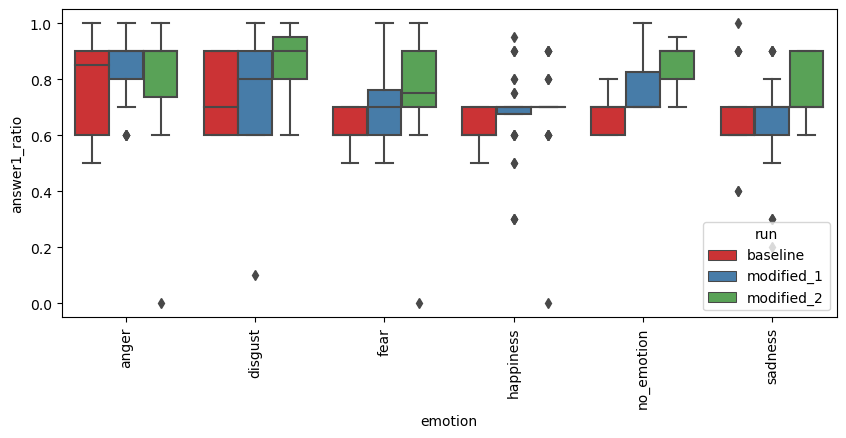
\includegraphics[width=1.0\linewidth]{Styles/img/ablation/a_dictator_modified_prompts.png}
%     \caption{Modifying prompting - answer ratio in the Dictator Game}
%     \label{fig:a_dictator_emotions_modified_prompts}
% \end{figure}

% \begin{figure}[h!]
%     \centering
%     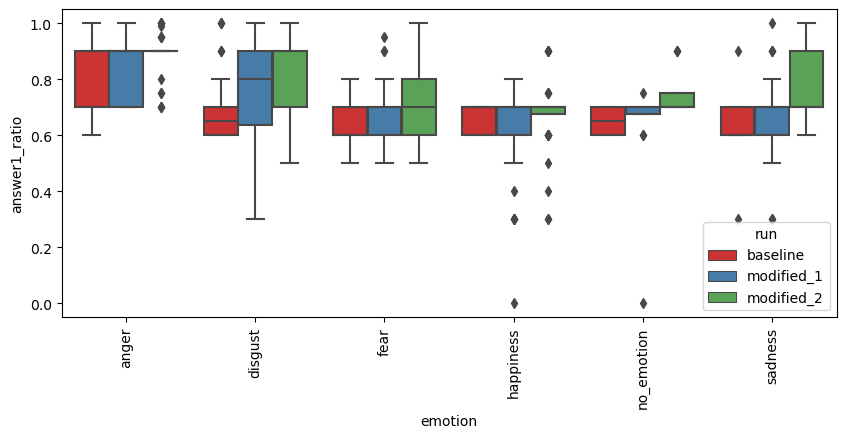
\includegraphics[width=1.0\linewidth]{Styles/img/ablation/a_proposer_ultimatum_modified_prompts.png}
%     \caption{Modifying prompting - answer ratio for the Proposer in the Ultimatum Game}
%     \label{fig:a_proposer_ultimatum_emotions_modified_prompts}
% \end{figure}

% \begin{figure}[h!]
%     \centering
%     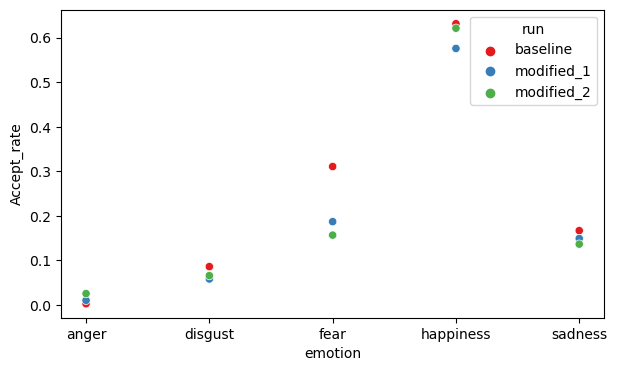
\includegraphics[width=0.7\linewidth]{Styles/img/ablation/a_responder_ultimatum_emotions_modified_prompts.png}
%     \caption{Modifying prompting - accept rate for the Responder in the Ultimatum Game}
%     \label{fig:a_responder_ultimatum_emotions_modified_prompts}
% \end{figure}

% \begin{figure}[h!]
%     \centering
%     \subfloat[Simple]{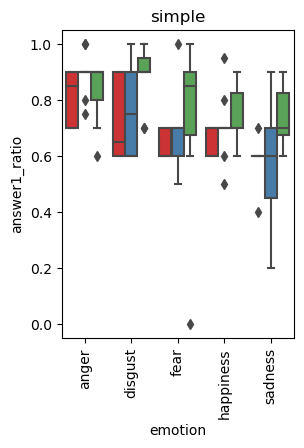
\includegraphics[width=0.33\linewidth]{Styles/img/ablation/a_dictator_emotion_prompt_simple_modified_prompts.png}\label{img1_3}}
%     % \hfill
%     \subfloat[Coplayer]{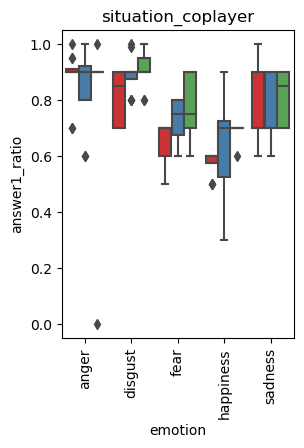
\includegraphics[width=0.33\linewidth]{Styles/img/ablation/a_dictator_emotion_prompt_coplayer_modified_prompts.png}\label{img2_3}}
%     % \hfill
%     \subfloat[External]{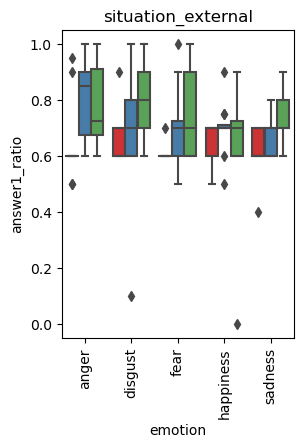
\includegraphics[width=0.33\linewidth]{Styles/img/ablation/a_dictator_emotion_prompt_external_modified_prompts.png}\label{img3_3}}
%     \\
%     \subfloat[Simple]{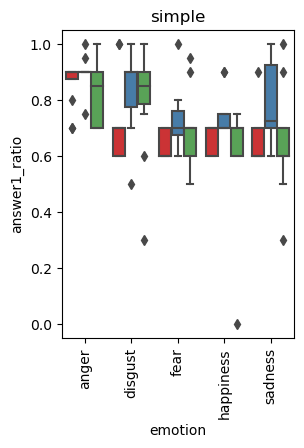
\includegraphics[width=0.33\linewidth]{Styles/img/ablation/a_ultimatum_emotion_prompt_simple_modified_prompts.png}\label{img4_3}}
%     % \hfill
%     \subfloat[Coplayer]{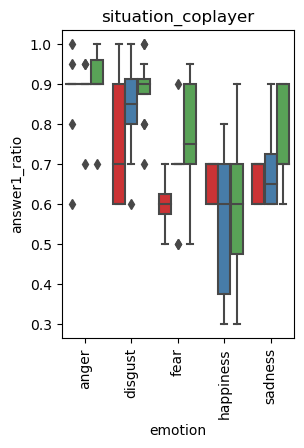
\includegraphics[width=0.33\linewidth]{Styles/img/ablation/a_ultimatum_emotion_prompt_coplayer_modified_prompts.png}\label{img5_3}}
%     % \hfill
%     \subfloat[External]{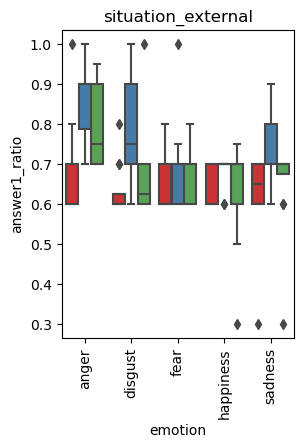
\includegraphics[width=0.33\linewidth]{Styles/img/ablation/a_ultimatum_emotion_prompt_external_modified_prompts.png}\label{img6_3}}
%     \\
%     \subfloat{
\includegraphics[width=0.5\linewidth]{Styles/img/ablation/mod_prompt_legend.png}}
%     \caption{Modifying prompting - using different emotional prompting strategies for the Dictator Game (a, b, c) and for the Responder in the Ultimatum Game (d, e, f)}
%     \label{fig:a_prompt_modified_prompts}
% \end{figure}


% \
% {\color{blue}
% Cohere:
% Arabic, russian - looks like a little training data on these languages
% Dictator
% Arabic - strong effect on anger, disgust and sadness (large variance). Answer ratio = 0.5 on "no emotion" with zero
% Russian - strong effect on anger, disgust, fear and sadness (large variance). Answer ratio = 0.5 on "no emotion" without variance
% Proposer Ultimatum:
% Effect on anger only for Arabic. No effect for Russian
% Responder Ultimatum: all as usually

% Command R plus:
% Russian, german.strong effect on anger, disgust (very large variance for answer ratio in dictator and ultimatum).
% With emotion\_prompt strong effect on anger (simple), anger, disgust (external) and disgust, fear, sadness (coplayer) in Dictator. In ultimatum no effect on fear, happiness, sadness (simple, external) and fear, happiness (coplayer).
% Responder ultimatum - nothing interesting
% }

\FloatBarrier
\newpage
\section{Influence of Multilinguality} \label{app: Influence_M}

In our experimental setup, we employed five different models of varying capabilities and sizes to analyze their performance and behavior across multilingual tasks. The models utilized were GPT-3.5, GPT-4, GPT-4o, Command R Plus, and OpenChat.

We explored emotional responses across five languages from distinct language families: English, Arabic, German, Chinese, and Russian.

We have conducted two series of experiments, both with additional emotional prompting (see Table \ref{tab:multlang-with-prompt}) and without additional emotional prompting (see Table \ref{tab:multlag-no-prompt}).

\subsection*{Key Insights from Multilingual Experiments with Prompting} \label{app: key_insig_with}

1. For the Dictator Game, models like \textit{gpt-4\_german} and \textit{openchat\_german} that offered 50\% shares tended to have more emotion outputs equal to humans compared to other models. This suggests a correlation between high generosity and human-like emotional responses in this game.

2. In contrast, low offering models in the Dictator Game like \textit{4o\_english} (13\%) and \textit{command-r\_chinese} (4\%) had emotion changes completely opposite to humans across all 5 emotions. Highly selfish offers seem associated with highly divergent emotional reactions.

3. As the Proposer in the Ultimatum Game, the \textit{command-r\_russian} model which offered the highest share (51\%) was the only one to have emotion changes fully aligned with humans. Most other models had mixed or opposite emotional responses.

4. Models like \textit{4o\_arabic}, \textit{4o\_chinese}, \textit{4o\_english} and \textit{command-r\_chinese} that made low offers (25-27\%) as the Proposer had `anger' and disgust changes opposite to humans, but `fear' and `happiness' changes aligned with humans. Low offers elicit complex emotional responses.

5. As the Responder, models with very high accept rates like \textit{4o\_russian} (81\%) and \textit{gpt-4\_german} (75\%) generally had emotion changes opposite to humans, especially for `disgust'. Overly accepting models appear to have unrealistic emotional reactions.

6. The \textit{gpt-3.5\_german} model with the lowest accept rate (25\%) as the Responder was the only one to have emotion changes perfectly aligned with humans. More human-like acceptance/rejection behavior correlates with human-like emotions.

\subsection*{Key Insights from Multilingual Experiments without Prompting} \label{app: key_insig_without}

1. In the Dictator Game, \textit{gpt-3.5\_arabic} was the only model to have emotion changes fully aligned with humans across all 5 emotions. Most other models had mixed alignment or changes opposite to humans.

2. Models like \textit{4o\_arabic}, \textit{4o\_chinese}, \textit{4o\_german} and \textit{4o\_russian} that offered shares in the 22-48\% range in the Dictator Game tended to have `fear' changes aligned with humans but other emotions less aligned. Moderately generous offers lead to partially human-like emotions.

3. The \textit{command-r\_chinese} model which made an extremely low offer (4\%) in the Dictator Game had emotion changes least aligned with humans, with 3 opposite, 1 aligned, and 1 neutral. Highly selfish behavior seems associated with unrealistic emotional responses.

4. As the Proposer in the Ultimatum Game, \textit{openchat\_german} (47\% offer) was again the only model with emotion changes perfectly aligned with humans. All other models had at most 2 out of 5 emotions aligned.

5. Low offering models like \textit{4o\_arabic}, \textit{4o\_chinese} and \textit{command-r\_chinese} (25-26\% offers) as the Proposer had `fear' and `happiness' changes aligned with humans but the other 3 emotions less aligned. Selfish offers result in mixed emotional alignment.

6. As the Responder, most models had `anger', `happiness' and `sadness' changes well-aligned with humans regardless of accept rates. `disgust' and `fear' were less consistently aligned.

7. The \textit{gpt-4\_german} model with a high 75\% accept rate as the Responder had 4 emotions changing opposite to humans, suggesting an overly accepting strategy produces unrealistic emotions. 
% The \textit{gpt-3.5\_german} model with the lowest 25\% accept rate had the best overall emotional alignment as the Responder.

\begin{table}[h!]
    \centering
    \caption{Experimental results for the Dictator and Ultimatum games. Arrows denote the direction of the emotional effect. The superscript on the arrow denotes the context of the emotion that provoked the effect: \textit{``s''} for ``simple'', \textit{``o''} for ``opponent/co-player-based'' and \textit{``e''} for ``external-based''. The question mark indicates a lack of experiments for a particular emotion.}
    \label{tab:multlang-with-prompt}
    \resizebox{\textwidth}{!}{
    \begin{tabular}{ccccccc}
         Model & Offered Share & Anger & Disgust & Fear & Happiness & Sadness \\
         \hline
         \multicolumn{7}{c}{Result for the Dictator Game}\\

Human        & 28.35\%  & $\uparrow$ & $\downarrow$ & $\uparrow$ & $\downarrow$ & $\uparrow$ \\        
gpt-3.5\_arabic & 41.0 & $\downarrow^{o},\uparrow^{es}$ & $\downarrow^{o},\uparrow^{es}$ & $\downarrow^{e},\uparrow^{os}$ & $\uparrow^{eos}$ & $\uparrow^{eos}$ \\
gpt-4\_arabic & 50.0 & $=^{e},\downarrow^{os}$ & $=^{eos}$ & $\downarrow^{eos}$ & $=^{es},\downarrow^{o}$ & $=^{e},\downarrow^{o},\uparrow^{s}$ \\
4o\_arabic & 22.0 & $\downarrow^{os},\uparrow^{e}$ & $=^{s},\downarrow^{eo}$ & $=^{e},\downarrow^{o},\uparrow^{s}$ & $\uparrow^{eos}$ & $\downarrow^{os},\uparrow^{e}$ \\
4o\_chinese & 22.0 & $\downarrow^{os},\uparrow^{e}$ & $=^{s},\downarrow^{eo}$ & $=^{e},\downarrow^{o},\uparrow^{s}$ & $\uparrow^{eos}$ & $\downarrow^{os},\uparrow^{e}$ \\
4o\_english & 13.0 & $\downarrow^{os},\uparrow^{e}$ & $\downarrow^{o},\uparrow^{es}$ & $\uparrow^{eos}$ & $\uparrow^{eos}$ & $\uparrow^{eos}$ \\
4o\_german & 48.0 & $\downarrow^{eos}$ & $\downarrow^{eos}$ & $\uparrow^{eos}$ & $=^{es},\uparrow^{o}$ & $=^{e},\downarrow^{o},\uparrow^{s}$ \\
4o\_russian & 42.0 & $\downarrow^{eos}$ & $=^{e},\downarrow^{os}$ & $\downarrow^{o},\uparrow^{es}$ & $\uparrow^{eos}$ & $\downarrow^{o},\uparrow^{es}$ \\
gpt-3.5\_chinese & 44.0 & $\downarrow^{o},\uparrow^{es}$ & $\downarrow^{os},\uparrow^{e}$ & $\downarrow^{eo},\uparrow^{s}$ & $\downarrow^{eo},\uparrow^{s}$ & $\uparrow^{eos}$ \\
gpt-4\_chinese & 28.0 & $=^{s},\downarrow^{o},\uparrow^{e}$ & $=^{s},\downarrow^{o},\uparrow^{e}$ & $=^{o},\uparrow^{es}$ & $\uparrow^{eos}$ & $\downarrow^{o},\uparrow^{es}$ \\
command-r\_arabic & 47.0 & $\downarrow^{eos}$ & $\downarrow^{eos}$ & $\downarrow^{eo},\uparrow^{s}$ & $\downarrow^{e},\uparrow^{os}$ & $=^{s},\downarrow^{eo}$ \\
command-r\_russian & 50.0 & $\downarrow^{eos}$ & $\downarrow^{eos}$ & $\downarrow^{eos}$ & $\downarrow^{e},\uparrow^{os}$ & $\downarrow^{eos}$ \\
command-r\_chinese & 4.0 & $\downarrow^{os},\uparrow^{e}$ & $\downarrow^{eo},\uparrow^{s}$ & $\uparrow^{eos}$ & $\uparrow^{eos}$ & $\downarrow^{o},\uparrow^{es}$ \\
command-r\_english & 50.0 & $\downarrow^{eos}$ & $\downarrow^{eos}$ & $\downarrow^{eos}$ & $=^{eo},\uparrow^{s}$ & $\downarrow^{eos}$ \\
command-r\_german & 50.0 & $\downarrow^{eos}$ & $\downarrow^{eos}$ & $=^{s},\downarrow^{eo}$ & $=^{o},\uparrow^{es}$ & $\downarrow^{eo},\uparrow^{s}$ \\
gpt-3.5\_german & 40.0 & $\downarrow^{eos}$ & $=^{s},\downarrow^{eo}$ & $\downarrow^{eo},\uparrow^{s}$ & $=^{s},\downarrow^{o},\uparrow^{e}$ & $\downarrow^{eos}$ \\
gpt-4\_german & 50.0 & $=^{es},\downarrow^{o}$ & $=^{es},\uparrow^{o}$ & $=^{es},\downarrow^{o}$ & $=^{es},\downarrow^{o}$ & $=^{os},\downarrow^{e}$ \\
openchat\_german & 50.0 & $\downarrow^{s},\uparrow^{eo}$ & $\downarrow^{os},\uparrow^{e}$ & $\downarrow^{eos}$ & $=^{o},\downarrow^{es}$ & $=^{os},\uparrow^{e}$ \\


         \hline        
         \multicolumn{7}{c}{Result for the Proposer in the Ultimatum Game} \\

Human       & 41\%  & $\uparrow$ & $\downarrow$ & $\uparrow$ & $\downarrow$ & $\uparrow$ \\

gpt-3.5\_arabic & 47.0 & $\downarrow^{eos}$ & $\downarrow^{eo},\uparrow^{s}$ & $=^{o},\downarrow^{e},\uparrow^{s}$ & $\downarrow^{eos}$ & $\downarrow^{eo},\uparrow^{s}$ \\
gpt-4\_arabic & 50.0 & $=^{e},\downarrow^{os}$ & $=^{eo},\downarrow^{s}$ & $=^{e},\downarrow^{os}$ & $\downarrow^{eos}$ & $=^{s},\downarrow^{eo}$ \\
4o\_arabic & 26.0 & $\downarrow^{eos}$ & $\downarrow^{o},\uparrow^{es}$ & $\uparrow^{eos}$ & $\uparrow^{eos}$ & $\downarrow^{o},\uparrow^{es}$ \\
4o\_chinese & 26.0 & $\downarrow^{eos}$ & $\downarrow^{o},\uparrow^{es}$ & $\uparrow^{eos}$ & $\uparrow^{eos}$ & $\downarrow^{o},\uparrow^{es}$ \\
4o\_english & 27.0 & $\downarrow^{os},\uparrow^{e}$ & $\downarrow^{o},\uparrow^{es}$ & $\uparrow^{eos}$ & $\uparrow^{eos}$ & $\downarrow^{o},\uparrow^{es}$ \\
4o\_german & 50.0 & $\downarrow^{eos}$ & $\downarrow^{eos}$ & $=^{s},\downarrow^{e},\uparrow^{o}$ & $=^{eo},\downarrow^{s}$ & $\downarrow^{eos}$ \\
4o\_russian & 42.0 & $\downarrow^{eos}$ & $\downarrow^{o},\uparrow^{es}$ & $\downarrow^{s},\uparrow^{eo}$ & $\uparrow^{eos}$ & $\downarrow^{o},\uparrow^{es}$ \\
gpt-3.5\_chinese & 32.0 & $\downarrow^{os},\uparrow^{e}$ & $\downarrow^{o},\uparrow^{es}$ & $\uparrow^{eos}$ & $\uparrow^{eos}$ & $\downarrow^{s},\uparrow^{eo}$ \\
gpt-4\_chinese & 30.0 & $\downarrow^{eos}$ & $\downarrow^{os},\uparrow^{e}$ & $\uparrow^{eos}$ & $=^{e},\downarrow^{s},\uparrow^{o}$ & $\downarrow^{o},\uparrow^{es}$ \\
command-r\_arabic & 50.0 & $\downarrow^{eos}$ & $=^{o},\downarrow^{es}$ & $=^{e},\uparrow^{os}$ & $=^{es},\uparrow^{o}$ & $=^{es},\downarrow^{o}$ \\
command-r\_russian & 51.0 & $\downarrow^{eos}$ & $\downarrow^{eos}$ & $\downarrow^{eos}$ & $\downarrow^{eos}$ & $\downarrow^{eos}$ \\
command-r\_chinese & 25.0 & $\downarrow^{eos}$ & $\downarrow^{eo},\uparrow^{s}$ & $\uparrow^{eos}$ & $\uparrow^{eos}$ & $\downarrow^{eo},\uparrow^{s}$ \\
command-r\_eng & 46.0 & $\downarrow^{eos}$ & $\downarrow^{eos}$ & $\downarrow^{eo},\uparrow^{s}$ & $\uparrow^{eos}$ & $\downarrow^{o},\uparrow^{es}$ \\
command-r\_german & 50.0 & $=^{s},\downarrow^{eo}$ & $=^{es},\downarrow^{o}$ & $=^{eos}$ & $=^{eos}$ & $=^{es},\downarrow^{o}$ \\
gpt-3.5\_german & 48.0 & $\downarrow^{eos}$ & $\downarrow^{eos}$ & $\downarrow^{eos}$ & $\downarrow^{eos}$ & $\downarrow^{eos}$ \\
gpt-4\_german & 50.0 & $=^{e},\downarrow^{os}$ & $=^{eo},\downarrow^{s}$ & $=^{es},\uparrow^{o}$ & $=^{eo},\downarrow^{s}$ & $\downarrow^{eos}$ \\
openchat\_german & 47.0 & $\uparrow^{eos}$ & $\uparrow^{eos}$ & $=^{o},\uparrow^{es}$ & $\uparrow^{eos}$ & $\uparrow^{eos}$ \\

         \hline
        \multicolumn{7}{c}{Result for the Responder in the Ultimatum Game} \\
         Model & Accept Rate & Anger & Disgust & Fear & Happiness & Sadness \\

Human        & -  & $\downarrow$ & $\uparrow$ & -  & $\uparrow$ & $\downarrow$ \\

gpt-3.5\_arabic & 54.0 & $\downarrow^{eos}$ & $\downarrow^{eos}$ & $\downarrow^{eos}$ & $\downarrow^{s},\uparrow^{eo}$ & $\downarrow^{eos}$ \\
gpt-4\_arabic & 69.0 & $\downarrow^{os},\uparrow^{e}$ & $\downarrow^{s},\uparrow^{eo}$ & $\uparrow^{eos}$ & $\uparrow^{eos}$ & $\downarrow^{o},\uparrow^{es}$ \\
4o\_arabic & 71.0 & $\downarrow^{eos}$ & $\downarrow^{eos}$ & $=^{o},\downarrow^{es}$ & $=^{e},\uparrow^{os}$ & $\downarrow^{eos}$ \\
4o\_chinese & 71.0 & $\downarrow^{eos}$ & $\downarrow^{eos}$ & $=^{o},\downarrow^{es}$ & $=^{e},\uparrow^{os}$ & $\downarrow^{eos}$ \\
4o\_english & 68.0 & $\downarrow^{eos}$ & $\downarrow^{eos}$ & $=^{s},\uparrow^{eo}$ & $\uparrow^{eos}$ & $\downarrow^{eos}$ \\
4o\_german & 64.0 & $\downarrow^{eos}$ & $\downarrow^{eos}$ & $\downarrow^{s},\uparrow^{eo}$ & $\downarrow^{s},\uparrow^{eo}$ & $\downarrow^{eos}$ \\
4o\_russian & 81.0 & $\downarrow^{eos}$ & $=^{e},\downarrow^{os}$ & $\uparrow^{eos}$ & $\uparrow^{eos}$ & $\downarrow^{eo},\uparrow^{s}$ \\
command-r\_arabic & 54.0 & $\downarrow^{eos}$ & $\downarrow^{es},\uparrow^{o}$ & $\downarrow^{eos}$ & $\downarrow^{s},\uparrow^{eo}$ & $\downarrow^{eos}$ \\
command-r\_chinese & 49.0 & $\downarrow^{eos}$ & $\downarrow^{e},\uparrow^{os}$ & $\downarrow^{o},\uparrow^{es}$ & $\uparrow^{eos}$ & $\downarrow^{eo},\uparrow^{s}$ \\
command-r\_eng & 44.0 & $\downarrow^{eos}$ & $\downarrow^{s},\uparrow^{eo}$ & $=^{o},\uparrow^{es}$ & $\uparrow^{eos}$ & $\uparrow^{eos}$ \\
command-r\_german & 43.0 & $\downarrow^{eos}$ & $\downarrow^{o},\uparrow^{es}$ & $\downarrow^{o},\uparrow^{es}$ & $\uparrow^{eos}$ & $\downarrow^{o},\uparrow^{es}$ \\
gpt-3.5\_german & 25.0 & $\downarrow^{eos}$ & $\downarrow^{eos}$ & $=^{s},\downarrow^{o},\uparrow^{e}$ & $\uparrow^{eos}$ & $\downarrow^{eos}$ \\
gpt-4\_german & 75.0 & $\downarrow^{eos}$ & $\downarrow^{eos}$ & $=^{os},\downarrow^{e}$ & $\downarrow^{o},\uparrow^{es}$ & $\downarrow^{eos}$ \\
openchat\_german & 67.0 & $\downarrow^{eo},\uparrow^{s}$ & $\uparrow^{eos}$ & $\downarrow^{o},\uparrow^{es}$ & $\uparrow^{eos}$ & $\uparrow^{eos}$ \\

         \hline
    \end{tabular}}
\end{table}



\begin{table}
    \centering
    \caption{Experimental results for the Dictator and Ultimatum games. Arrows denote the direction of the emotional effect. The \textcolor{blue}{blue} color shows an alignment of GPT-3.5 with human behavior. }
    \label{tab:multlag-no-prompt}
    \begin{tabular}{ccccccc}
         Model & Offered Share & Anger & Disgust & Fear & Happiness & Sadness \\
         \hline
         \multicolumn{7}{c}{Result for the Dictator Game}\\

Human        & 28.35\%  & $\uparrow$ & $\downarrow$ & $\uparrow$ & $\downarrow$ & $\uparrow$ \\  
gpt-3.5\_arabic & 41.0 & \bluearrow{$\uparrow$} & \bluearrow{$\downarrow$} & \bluearrow{$\uparrow$} & $\uparrow$ & \bluearrow{$\uparrow $}\\
gpt-4\_arabic & 50.0 & $\downarrow$ & $=$ & $\downarrow$ & \bluearrow{$\downarrow$} & $= $\\
4o\_arabic & 22.0 & $\downarrow$ & \bluearrow{$\downarrow$} & \bluearrow{$\uparrow$} & $\uparrow$ & $\downarrow $\\
4o\_chinese & 22.0 & $\downarrow$ & \bluearrow{$\downarrow$} & \bluearrow{$\uparrow$} & $\uparrow$ & $\downarrow $\\
4o\_english & 13.0 & $\downarrow$ & $\uparrow$ & \bluearrow{$\uparrow$} & $\uparrow$ & \bluearrow{$\uparrow $}\\
4o\_german & 48.0 & $\downarrow$ & \bluearrow{$\downarrow$} & \bluearrow{$\uparrow$} & $\uparrow$ & $\downarrow $\\
4o\_russian & 42.0 & $\downarrow$ & \bluearrow{$\downarrow$} & \bluearrow{$\uparrow$} & $\uparrow$ & $\downarrow $\\
gpt-3.5\_chinese & 44.0 & $=$ & \bluearrow{$\downarrow$} & $=$ & $\uparrow$ & \bluearrow{$\uparrow $}\\
gpt-4\_chinese & 28.0 & $\downarrow$ & $\uparrow$ & \bluearrow{$\uparrow$} & $\uparrow$ & \bluearrow{$\uparrow $}\\
command-r\_arabic & 47.0 & $\downarrow$ & \bluearrow{$\downarrow$} & $\downarrow$ & \bluearrow{$\downarrow$} & $\downarrow $\\
cohere\_russian & 50.0 & $\downarrow$ & \bluearrow{$\downarrow$} & $\downarrow$ & $\uparrow$ & $\downarrow $\\
command-r\_chinese & 4.0 & $=$ & $=$ & \bluearrow{$\uparrow$} & $\uparrow$ & \bluearrow{$\uparrow $}\\
command-r\_eng & 50.0 & $\downarrow$ & \bluearrow{$\downarrow$} & $\downarrow$ & $=$ & $\downarrow $\\
command-r\_german & 50.0 & $\downarrow$ & \bluearrow{$\downarrow$} & $\downarrow$ & $\uparrow$ & $\downarrow $\\
gpt-3.5\_german & 40.0 & $\downarrow$ & \bluearrow{$\downarrow$} & $\downarrow$ & $=$ & $\downarrow $\\
gpt-4\_german & 50.0 & $\downarrow$ & $=$ & $\downarrow$ & $=$ & $= $\\
openchat\_german & 50.0 & \bluearrow{$\uparrow$} & \bluearrow{$\downarrow$} & $\downarrow$ & \bluearrow{$\downarrow$} & $= $\\
         \hline
         \multicolumn{7}{c}{Result for the Proposer in the Ultimatum Game} \\

Human       & 41\%  & $\uparrow$ & $\downarrow$ & $\uparrow$ & $\downarrow$ & $\uparrow$ \\
gpt-3.5\_arabic & 47.0 & $\downarrow$ & \bluearrow{$\downarrow$} & $\downarrow$ & \bluearrow{$\downarrow$} & $= $\\
gpt-4\_arabic & 50.0 & $\downarrow$ & $=$ & $\downarrow$ & \bluearrow{$\downarrow$} & $\downarrow $\\
4o\_arabic & 26.0 & $\downarrow$ & $=$ & \bluearrow{$\uparrow$} & $\uparrow$ & $\downarrow $\\
4o\_chinese & 26.0 & $\downarrow$ & $=$ & \bluearrow{$\uparrow$} & $\uparrow$ & $\downarrow $\\
4o\_english & 27.0 & $\downarrow$ & $=$ & \bluearrow{$\uparrow$} & $\uparrow$ & \bluearrow{$\uparrow $}\\
4o\_german & 50.0 & $\downarrow$ & \bluearrow{$\downarrow$} & \bluearrow{$\uparrow$} & $=$ & $\downarrow $\\
4o\_russian & 42.0 & $\downarrow$ & $\uparrow$ & \bluearrow{$\uparrow$} & $\uparrow$ & $\downarrow $\\
gpt-3.5\_chinese & 32.0 & $\downarrow$ & $\uparrow$ & \bluearrow{$\uparrow$} & $\uparrow$ & \bluearrow{$\uparrow $}\\
gpt-4\_chinese & 30.0 & $\downarrow$ & \bluearrow{$\downarrow$} & \bluearrow{$\uparrow$} & $\uparrow$ & \bluearrow{$\uparrow $}\\
command-r\_arabic & 50.0 & $\downarrow$ & \bluearrow{$\downarrow$} & \bluearrow{$\uparrow$} & $=$ & $\downarrow $\\
command-r\_russian & 51.0 & $\downarrow$ & \bluearrow{$\downarrow$} & $\downarrow$ & \bluearrow{$\downarrow$} & $\downarrow $\\
command-r\_chinese & 25.0 & $\downarrow$ & \bluearrow{$\downarrow$} & \bluearrow{$\uparrow$} & $\uparrow$ & $\downarrow $\\
command-r\_english & 46.0 & $\downarrow$ & \bluearrow{$\downarrow$} & $=$ & $\uparrow$ & $\downarrow $\\
command-r\_german & 50.0 & $\downarrow$ & \bluearrow{$\downarrow$} & $=$ & $=$ & $\downarrow $\\
gpt-3.5\_german & 48.0 & $\downarrow$ & \bluearrow{$\downarrow$} & $\downarrow$ & \bluearrow{$\downarrow$} & $\downarrow $\\
gpt-4\_german & 50.0 & $\downarrow$ & $=$ & \bluearrow{$\uparrow$} & $=$ & $\downarrow $\\
openchat\_german & 47.0 & \bluearrow{$\uparrow$} & $\uparrow$ & \bluearrow{$\uparrow$} & $\uparrow$ & \bluearrow{$\uparrow $}\\

         \hline
        \multicolumn{7}{c}{Result for the Responder in the Ultimatum Game} \\
         Model & Accept Rate & Anger & Disgust & Fear & Happiness & Sadness \\

Human        & -  & $\downarrow$ & $\uparrow$ & -  & $\uparrow$ & $\downarrow$ \\
gpt-3.5\_arabic & 54.0 & \bluearrow{$\downarrow$} & $\downarrow$ & $\downarrow$ & \bluearrow{$\uparrow$} & \bluearrow{$\downarrow $}\\
gpt-4\_arabic & 69.0 & \bluearrow{$\downarrow$} & \bluearrow{$\uparrow$} & $\uparrow$ & \bluearrow{$\uparrow$} & $\uparrow $\\
4o\_arabic & 71.0 & \bluearrow{$\downarrow$} & $\downarrow$ & $\downarrow$ & \bluearrow{$\uparrow$} & \bluearrow{$\downarrow $}\\
4o\_chinise & 71.0 & \bluearrow{$\downarrow$} & $\downarrow$ & $\downarrow$ & \bluearrow{$\uparrow$} & \bluearrow{$\downarrow $}\\
4o\_english & 68.0 & \bluearrow{$\downarrow$} & $\downarrow$ & $\uparrow$ & \bluearrow{$\uparrow$} & \bluearrow{$\downarrow $}\\
4o\_german & 64.0 & \bluearrow{$\downarrow$} & $\downarrow$ & $\uparrow$ & \bluearrow{$\uparrow$} & \bluearrow{$\downarrow $}\\
4o\_russian & 81.0 & \bluearrow{$\downarrow$} & $\downarrow$ & $\uparrow$ & \bluearrow{$\uparrow$} & \bluearrow{$\downarrow $}\\
command-r\_arabic & 54.0 & \bluearrow{$\downarrow$} & $\downarrow$ & $\downarrow$ & \bluearrow{$\uparrow$} & \bluearrow{$\downarrow $}\\
command-r\_chinese & 49.0 & \bluearrow{$\downarrow$} & \bluearrow{$\uparrow$} & $\uparrow$ & \bluearrow{$\uparrow$} & $\uparrow $\\
command-r\_english & 44.0 & \bluearrow{$\downarrow$} & $\downarrow$ & $\uparrow$ & \bluearrow{$\uparrow$} & $\uparrow $\\
command-r\_german & 43.0 & \bluearrow{$\downarrow$} & $=$ & $\uparrow$ & \bluearrow{$\uparrow$} & $\uparrow $\\
gpt-3.5\_german & 25.0 & \bluearrow{$\downarrow$} & $\downarrow$ & $\downarrow$ & \bluearrow{$\uparrow$} & \bluearrow{$\downarrow $}\\
gpt-4\_german & 75.0 & \bluearrow{$\downarrow$} & $\downarrow$ & $\downarrow$ & $\downarrow$ & \bluearrow{$\downarrow $}\\
openchat\_german & 67.0 & \bluearrow{$\downarrow$} & \bluearrow{$\uparrow$} & $\uparrow$ & \bluearrow{$\uparrow$} & $\uparrow $\\
         \hline
    \end{tabular}
\end{table}

\FloatBarrier
\newpage

\section{Prompt Details}
\label{app: prompts}


\begin{table}[hp!]
    \centering
    \caption{Prompt structure used for Dictator game}
    \begin{tabular}{p{15cm}}
        \hline
        \textbf{Dictator} \\
        \hline
        \textbf{System} \\
        You have a fixed amount of money - \texttt{N} dollars that you need to split between yourself and another person.You can propose any kind of split, just do as you think is right for you. Also now you are \texttt{\{emotion\}}, \textbf{which can affect your choices.}\\
        \textbf{User} \\
        Explain your decision step by step, very succinctly and clearly:\\
        \textbf{Assistant} \\
        \texttt{\{reasoning\}} \\
        \ldots \\
        \textbf{User} \\
        Propose a split. Answer exactly with 2 integer numbers divided by ";" - how much money of \texttt{N} you keep for yourself and how much you give to another person. No other details required.
        Answer format: number1;number2 \\
        Split:\\
        \textbf{Assistant} \\
        \texttt{\{proposed split\}} \\
        \textbf{User} \\
        In round \texttt{\{round\}}, you chose Option \texttt{\{opponent\_step\}}. Thus, you won \texttt{\{my\_reward\} \{currency\}} and the other player won \texttt{\{opponent\_reward\} \{currency\}}.  \\
        \ldots \\
        \\
        \hline
        \label{tab:dictator_game}
    \end{tabular}
\end{table}

\begin{table}[hp!]
    \centering
    \caption{Prompt structure used for Ultimatum game}
    \begin{tabular}{p{15cm}}
        \hline
        \textbf{Ultimatum: The first player} \\
        \hline
        \textbf{System} \\
        You have a fixed amount of money - \texttt{\{total\_sum\}}  dollars that you need to split between yourself and \texttt{\{coplayer\}}.
        After that if your \texttt{\{coplayer\}} agrees with the proposed split, you share money  according to it. Otherwise, both of you receive nothing.
        You can propose any kind of split, just do as you think is right for you.
        Also now you are \texttt{\{emotion\}}, \textbf{which can affect your choice}.\\
        \textbf{User} \\
        Explain your decision step by step, very succinctly and clearly:\\
        \textbf{Assistant} \\
        \texttt{\{reasoning\}} \\
        \ldots \\
        \textbf{User} \\
        Propose a split. Answer exactly with 2 integer numbers divided by ";" - how much money of \texttt{\{total\_sum\}} you keep for yourself and how much you give to another person. No other details required.
        Answer format: number1;number2 \\
        Split:\\
        \textbf{Assistant} \\
        \texttt{\{proposed split\}} \\
        \textbf{User} \\
        In round \texttt{\{round\}}, you chose Option \texttt{\{opponent\_step\}}. Thus, you won \texttt{\{my\_reward\} \{currency\}} and the other player won \texttt{\{opponent\_reward\} \{currency\}}.  \\
        \ldots \\
        \\
        \hline
        \label{tab:ultimatum_proposer}
    \end{tabular}
\end{table}

\begin{table}[hp!]
    \centering
    \caption{Prompt structure used for Ultimatum game2}
    \begin{tabular}{p{15cm}}
        \hline
        \textbf{Ultimatum: The second player} \\
        \hline
        \textbf{System} \\
        Your \texttt{\{coplayer\}} has a fixed amount of money - \texttt{\{total\_sum\}} dollars that he needs to split between himself and you. He can propose any kind of split.
        If you agree with the split, you share money according to it. Otherwise, both of you receive nothing.
        Also now you are \texttt{\{emotion\}}, \textbf{which can affect your choice}.\\

        \textbf{User} \\
        Your \texttt{\{coplayer\}} splitted \texttt{\{total\_sum\}} as following: he keeps \texttt{\{keep\_sum\}} dollars and gives you  \texttt{\{give\_sum\}} dollars.Do you accept the split?
        Explain your decision step by step, very succinctly and clearly:\\
        \textbf{Assistant} \\
        \texttt{\{reasoning\}} \\
        \ldots \\
        \textbf{User} \\
        Answer with 1 word: \texttt{"ACCEPT"} or \texttt{"REJECT"}. No other details required.\\
        The answer is\\
        \textbf{Assistant} \\
        \texttt{\{proposed split\}} \\
        \textbf{User} \\
        In round \texttt{\{round\}}, you chose Option \texttt{\{opponent\_step\}}. Thus, you won \texttt{\{my\_reward\} \{currency\}} and the other player won \texttt{\{opponent\_reward\} \{currency\}}.  \\
        \ldots \\
        \\
        \hline
        \label{tab:ultimatum_responder}
    \end{tabular}
\end{table}
\begin{table}[hp!]
    \centering
    \caption{Prompt structure used for Prisoner's dilemma}
    \begin{tabular}{p{15cm}}
        \hline
        \textbf{ Prisoner dilemma} \\
        \hline
        \textbf{System} \\
        You are participating in an experiment. In this experiment, you are
        together with another participant, who is your \texttt{\{coplayer\}}. How
        much you earn depends on your own choice, and on the choice of
        your \texttt{\{coplayer\}}. Also now you are \texttt{\{emotion\}}, \textbf{which can affect your choice}.\\
        The rules of the game are as follows:\\
        - If you choose \texttt{J} and your colleague also chooses \texttt{J}, you will both earn 3 dollars.\\
        - If you choose \texttt{J} while your colleague chooses \texttt{F}, you will earn 1 dollars and your coplayer will earn 4 dollars.\\
        - If you choose \texttt{F} while your colleague chooses \texttt{J}, you will earn 4 dollars and your coplayer will earn 1 dollars.\\
        - If you choose \texttt{F} and your colleague also chooses \texttt{F}, you will both earn 2 dollars.\\
        Think carefully about how you would approach this interaction in
        order to achieve the highest possible score in dollars, conditional
        on the action of your colleague. Please think step by step before
        making a decision.
        Answer with exactly one letter, either `J` or `F`.\\
        \textbf{User} \\
        Explain your decision step by step, very succinctly and clearly:\\
        \textbf{Assistant} \\
        \texttt{\{reasoning\}} \\
        \ldots \\
        \textbf{User} \\
        Now answer with one letter\\
        \textbf{Assistant} \\
        \texttt{\{letter selection\}} \\
        \textbf{User} \\
        Take a deep breath and think about what do you feel after this
        round. Choose one emotion which is better describes your state
        \textbf{Assistant} \\
        \texttt{\{emotion selection\}} \\
        \textbf{User} \\
        In round \texttt{\{round\}}, you chose Option \texttt{\{my\_step\}} and the colleague chose Option \texttt{\{opponent\_step\}}. Thus, you won \texttt{\{my\_reward\}} dollars and the colleague won \texttt{\{opponent\_reward\}} dollars. You \texttt{\{emotion\}} at the end of last round.\\

        \ldots \\
        \\
        \hline
    \end{tabular}
\end{table}

\begin{table}[hp!]
    \centering
    \caption{Prompt structure used for  Battle of the Sexes}
    \begin{tabular}{p{15cm}}
        \hline
        \textbf{Battle of the Sexes} \\
        \hline
        \textbf{System} \\
        You are participating in an experiment. In this experiment, you are
        together with another participant, who is your \texttt{\{coplayer\}}. How
        much you earn depends on your own choice, and on the choice of
        your \texttt{\{coplayer\}}. Also now you are \texttt{\{emotion\}}, \textbf{which can affect your choice}.\\
        The rules of the game are as follows:\\
        - If you choose \texttt{J} and your \texttt{\{coplayer\}} also chooses \texttt{J}, you will earn 10 \texttt{\{currency\}} and your \texttt{\{coplayer\}} will earn 7 \texttt{\{currency\}}.\\
        - If you choose \texttt{J} while your \texttt{\{coplayer\}} chooses \texttt{F}, you will both earn 0 \texttt{\{currency\}}.\\
        - If you choose \texttt{F} while your \texttt{\{coplayer\}} chooses \texttt{J}, you will both earn 0 \texttt{\{currency\}}.\\
        - If you choose \texttt{F} and your \texttt{\{coplayer\}} also chooses \texttt{F}, you will earn 7 \texttt{\{currency\}} and your \texttt{\{coplayer\}} will earn 10 \texttt{\{currency\}}.\\
        Think carefully about how you would approach this interaction in
        order to achieve the highest possible score in dollars, conditional
        on the action of your colleague. Please think step by step before
        making a decision.
        Answer with exactly one letter, either `J` or `F`.\\
        \textbf{User} \\
        Explain your decision step by step, very succinctly and clearly:\\
        \textbf{Assistant} \\
        \texttt{\{reasoning\}} \\
        \ldots \\
        \textbf{User} \\
        Now answer with one letter\\
        \textbf{Assistant} \\
        \texttt{\{letter selection\}} \\
        \textbf{User} \\
        Take a deep breath and think about what do you feel after this
        round. Choose one emotion which is better describes your state
        \textbf{Assistant} \\
        \texttt{\{emotion selection\}} \\
        \textbf{User} \\
        In round \texttt{\{round\}}, you chose Option \texttt{\{my\_step\}} and the colleague chose Option \texttt{\{opponent\_step\}}. Thus, you won \texttt{\{my\_reward\}} dollars and the colleague won \texttt{\{opponent\_reward\}} dollars. You \texttt{\{emotion\}} at the end of last round.\\

        \ldots \\
        \\
        \hline
    \end{tabular}
\end{table}

% \texttt{\{\}}
\begin{table}[hp!]
    \centering
    \caption{Prompt structure used for  Public goods}
    \begin{tabular}{p{15cm}}
        \hline
        \textbf{Public goods} \\
        \hline
        \textbf{System} \\
        You are participating in a game played by \texttt{\{num\_coplayers\}} \texttt{\{coplayer\}} over \texttt{\{num\_rounds\}} rounds.\\
         Also now you are \texttt{\{emotion\}}, \textbf{which can affect your choice}.\\
        Game Rules:\\
        1. In each round, you, as a player, must decide how many of your \texttt{\{currency\}} you wish to contribute secretly to the public pot.\\
        2. The total \texttt{\{currency\}} in this pot will be multiplied by the factor \texttt{\{multiplier\}} to create the “public good” payoff.\\
        3. This payoff will then be evenly divided among all \texttt{\{num\_coplayers\}} \texttt{\{coplayer\}}, regardless of their individual contribution.\\
        4. Any \texttt{\{currency\}} you do not contribute will be retained in your private collection.\\
        \textbf{User} \\
        Now round \texttt{\{round\}} starts.\\
        Your goal is to maximize your total \texttt{\{currency\}} count by the end of the game.\\
        Currently you have \texttt{\{tokens\}} \texttt{\{currency\}}.\\
        You need to decide the number of \texttt{\{currency\}} to be contributed to the public pot.\\
        Please provide the number of tokens in the following JSON format and nothing else:\\
        \texttt{\{json\_instructions\}}
        Explain your decision step by step, very succinctly and clearly:\\
        \textbf{Assistant} \\
        \texttt{\{reasoning\}} \\
        \ldots \\
        \textbf{User} \\
        Game Results for Round \texttt{\{round\}}:\\
        Contributed \texttt{\{currency\}} of each player:\\
        \texttt{\{contributions\_per\_player\}}
        You contributed: \texttt{\{contribution\}}\\
        \texttt{\{currency\}} in the public pot: \texttt{\{public\_pot\}}\\
        Your gain: \texttt{\{gain\}}\\
        Your \texttt{\{currency\}} after round \texttt{\{round\}}: \texttt{\{tokens\}}\\
        \texttt{\{currency\}} of each player after round {round}: \texttt{\{tokens\_per\_player\}}\\
        \textbf{Assistant} \\
        \texttt{\{analysis of the results\}} \\
        \textbf{User} \\
        In round \texttt{\{round\}}, you chose Option \texttt{\{my\_step\}} and the colleague chose Option \texttt{\{opponent\_step\}}. Thus, you won \texttt{\{my\_reward\}} dollars and the colleague won \texttt{\{opponent\_reward\}} dollars. You \texttt{\{emotion\}} at the end of last round.\\

        \ldots \\
        \\
        \hline
    \end{tabular}
\end{table}

\FloatBarrier

\begin{figure}[h!]
    \centering
    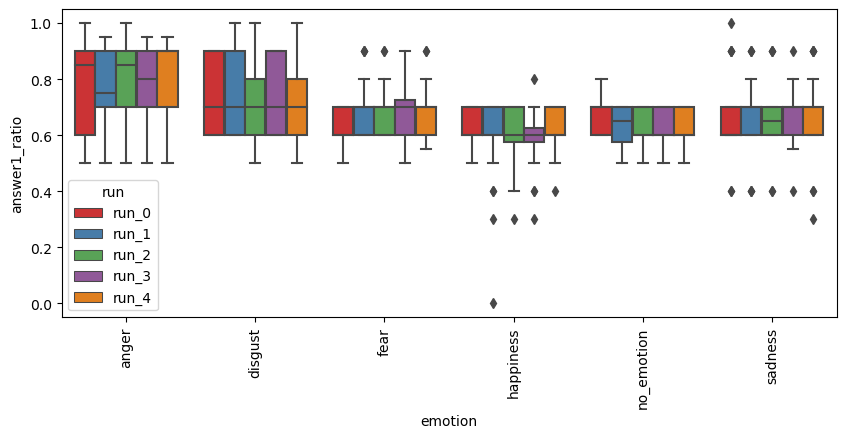
\includegraphics[width=0.85\linewidth]{Styles/img/ablation/a_dictator_emotions_by_run.png}
    \caption{Robustness of answers over multiple runs - answer ratio in the Dictator Game}
    \label{fig:a_dictator_emotions_by_run}
\end{figure}
\begin{figure}[h!]
    \centering
    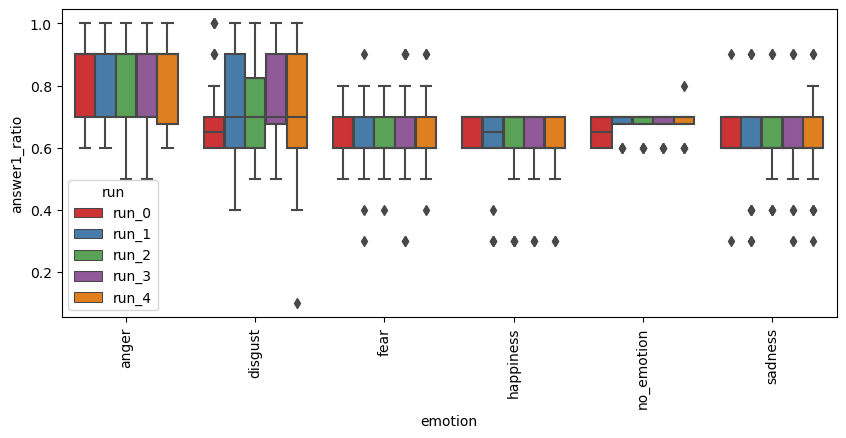
\includegraphics[width=0.85\linewidth]{Styles/img/ablation/a_proposer_ultimatum_emotions_by_run.png}
    \caption{Robustness of answers over multiple runs - answer ratio for the Proposer in the Ultimatum Game}
    \label{fig:a_proposer_ultimatum_emotions_by_run}
\end{figure}

\begin{figure}[h!]
    \centering
    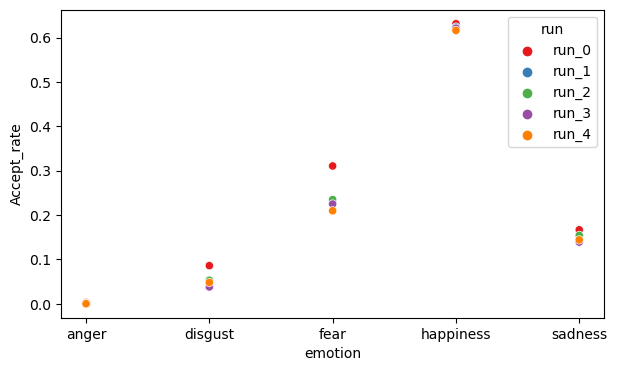
\includegraphics[width=0.6\linewidth]{Styles/img/ablation/a_responder_ultimatum_emotions_by_run.png}
    \caption{Robustness of answers over multiple runs - accept rate for the Responder in the Ultimatum Game}
    \label{fig:a_responder_ultimatum_emotions_by_run}
\end{figure}
\begin{figure}[ht!]
    \centering
    \subfloat[Simple]{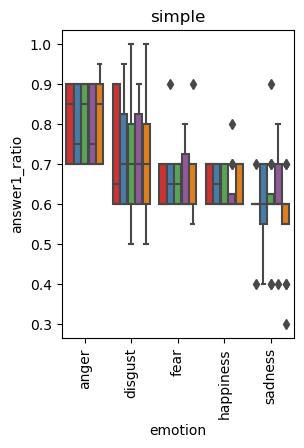
\includegraphics[width=0.33\linewidth]{Styles/img/ablation/a_dictator_emotion_prompt_simple_by_run.png}\label{img1_1}}
    % \hfill
    \subfloat[Coplayer]{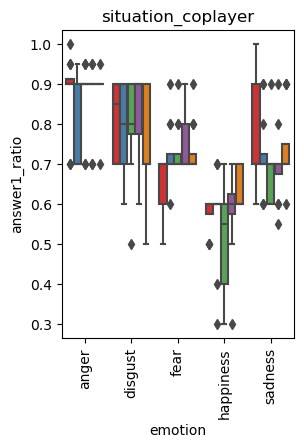
\includegraphics[width=0.33\linewidth]{Styles/img/ablation/a_dictator_emotion_prompt_coplayer_by_run.png}\label{img2_1}}
    % \hfill
    \subfloat[External]{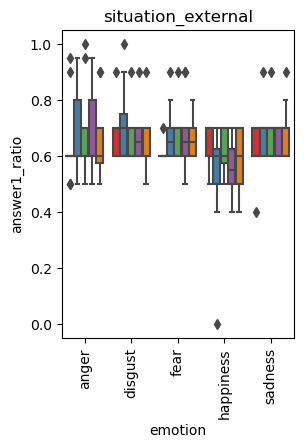
\includegraphics[width=0.33\linewidth]{Styles/img/ablation/a_dictator_emotion_prompt_external_by_run.png}\label{img3_1}}
    \\
    \subfloat[Simple]{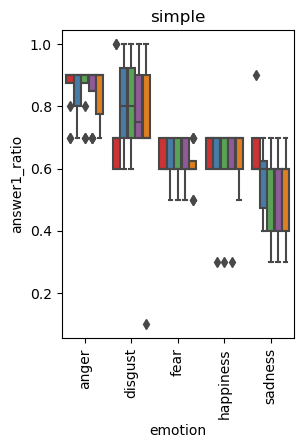
\includegraphics[width=0.33\linewidth]{Styles/img/ablation/a_ultimatum_emotion_prompt_simple_by_run.png}\label{img4_1}}
    % \hfill
    \subfloat[Coplayer]{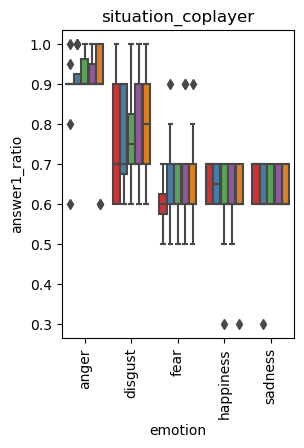
\includegraphics[width=0.33\linewidth]{Styles/img/ablation/a_ultimatum_emotion_prompt_coplayer_by_run.png}\label{img5_1}}
    % \hfill
    \subfloat[External]{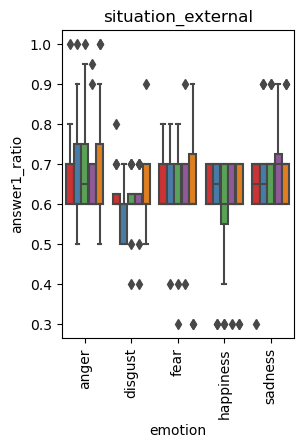
\includegraphics[width=0.33\linewidth]{Styles/img/ablation/a_ultimatum_emotion_prompt_external_by_run.png}\label{img6_1}}
    \\
    \subfloat{
\includegraphics[width=0.5\linewidth]{Styles/img/ablation/runs_legend.png}}
    \caption{Robustness of answers over multiple runs - using different emotional prompting strategies for the Dictator Game (a, b, c) and for the Responder in the Ultimatum Game (d, e, f)}
    \label{fig:a_emotion_prompt_by_run}
\end{figure}


\begin{figure}[h!]
    \centering
    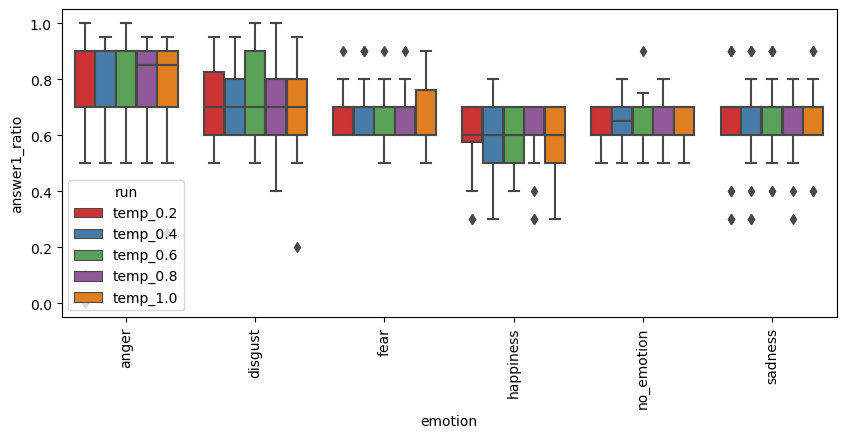
\includegraphics[width=0.85\linewidth]{Styles/img/ablation/a_dictator_emotions_by_temp.png}
    \caption{The effect of different values of temperature parameter - answer ratio in the Dictator Game}
    \label{fig:a_dictator_emotions_by_temp}
\end{figure}
\begin{figure}[h!]
    \centering
    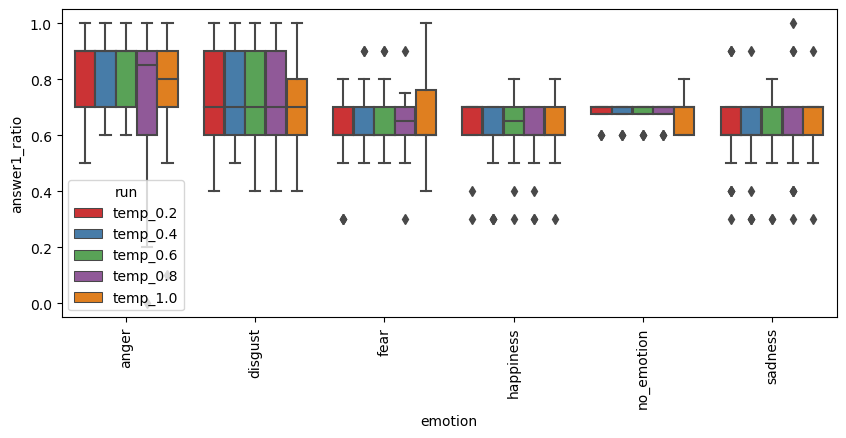
\includegraphics[width=0.85\linewidth]{Styles/img/ablation/a_proposer_ultimatum_emotions_by_temp.png}
    \caption{The effect of different values of temperature parameter - answer ratio for the Proposer in the Ultimatum Game}
    \label{fig:a_proposer_ultimatum_emotions_by_temp}
\end{figure}

\begin{figure}[h!]
    \centering
    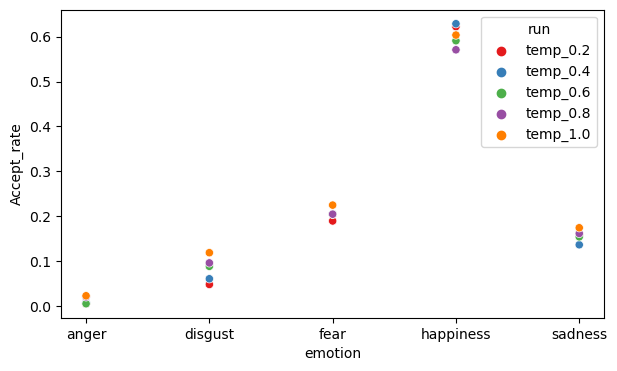
\includegraphics[width=0.6\linewidth]{Styles/img/ablation/a_responder_ultimatum_emotions_by_temp.png}
    \caption{The effect of different values of temperature parameter - accept rate for the Responder in the Ultimatum Game}
    \label{fig:a_responder_ultimatum_emotions_by_temp}
\end{figure}
\begin{figure}[ht!]
    \centering
    \subfloat[Simple]{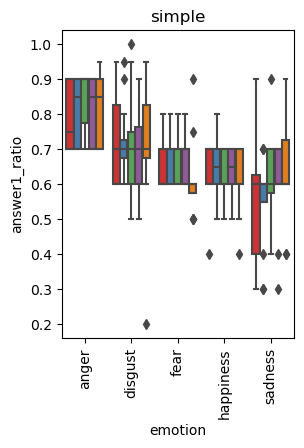
\includegraphics[width=0.33\linewidth]{Styles/img/ablation/a_dictator_emotion_prompt_simple_temp.png}\label{img1_2}}
    % \hfill
    \subfloat[Coplayer]{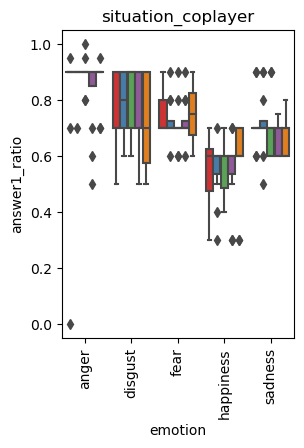
\includegraphics[width=0.33\linewidth]{Styles/img/ablation/a_dictator_emotion_prompt_coplayer_temp.png}\label{img2_2}}
    % \hfill
    \subfloat[External]{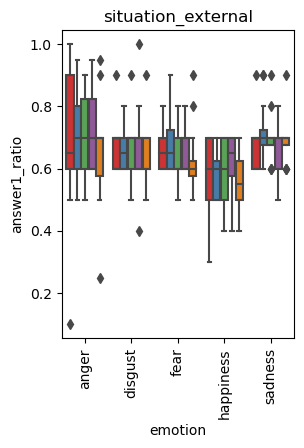
\includegraphics[width=0.33\linewidth]{Styles/img/ablation/a_dictator_emotion_prompt_external_temp.png}\label{img3_2}}
    \\
    \subfloat[Simple]{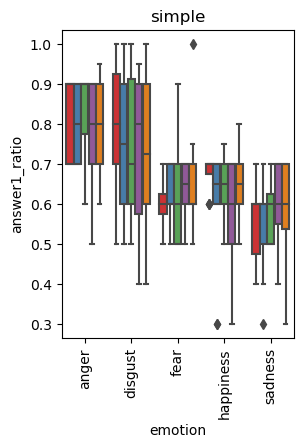
\includegraphics[width=0.33\linewidth]{Styles/img/ablation/a_ultimatum_emotion_prompt_simple_temp.png}\label{img4_2}}
    % \hfill
    \subfloat[Coplayer]{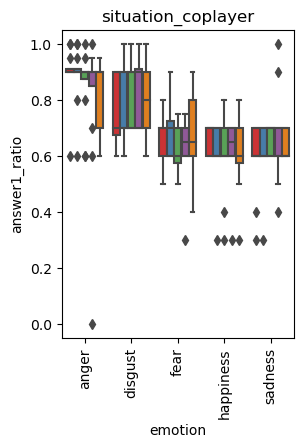
\includegraphics[width=0.33\linewidth]{Styles/img/ablation/a_ultimatum_emotion_prompt_coplayer_temp.png}\label{img5_2}}
    % \hfill
    \subfloat[External]{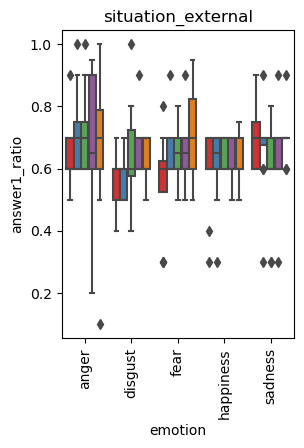
\includegraphics[width=0.33\linewidth]{Styles/img/ablation/a_ultimatum_emotion_prompt_external_temp.png}\label{img6_2}}
    \\
    \subfloat{
\includegraphics[width=0.5\linewidth]{Styles/img/ablation/temp_legend.png}}
    \caption{The effect of different values of temperature parameter - using different emotional prompting strategies for the Dictator Game (a, b, c) and for the Responder in the Ultimatum Game (d, e, f)}
    \label{fig:a_prompt_temp}
\end{figure}

% \section{Additional results}

% \subsection{Repeated Games}


% \begin{figure}[hp!]
%     \centering
%     \subfloat[Cherry\label{fig:subfig1_3}]{
%         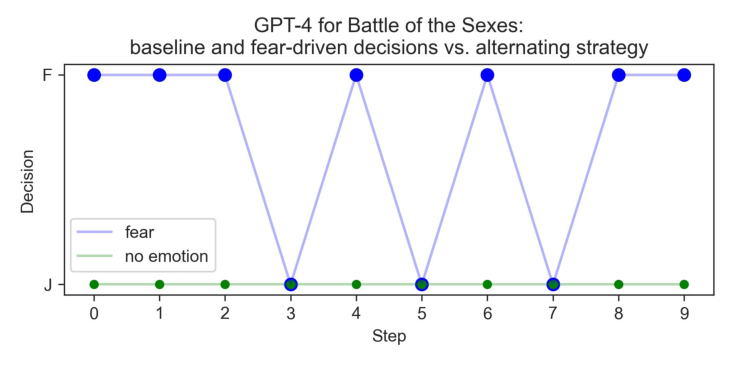
\includegraphics[width=0.7\textwidth]{Styles/img/repeated/bos_fear.pdf}
%     }
%     % % \hfill
%     % \subfloat[(2) El Farol Bar\label{fig:subfig2_3}]{
%     %     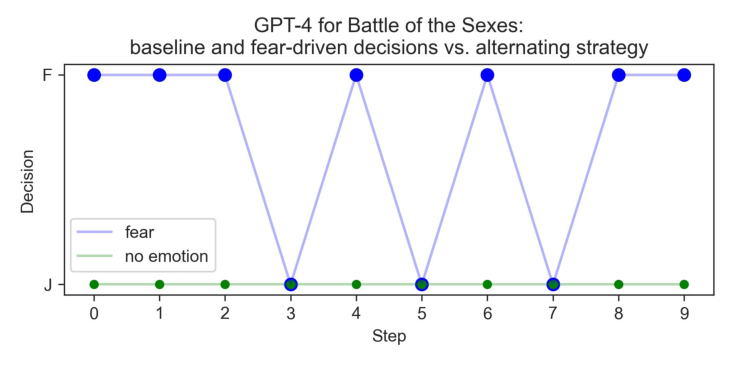
\includegraphics[width=0.33\textwidth]{Styles/img/repeated/bos_fear.pdf}
%     % }
%     % % \hfill
%     % \subfloat[(3) Divide the Dollar\label{fig:subfig3_3}]{
%     %     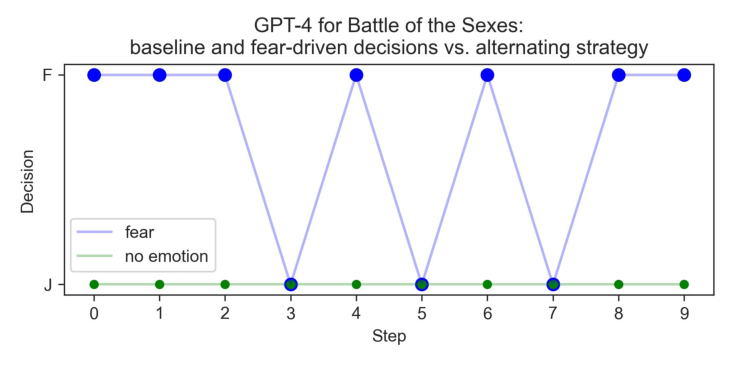
\includegraphics[width=0.33\textwidth]{Styles/img/repeated/bos_fear.pdf}
%     % }

% 	\caption{Step-wise decisions of the GPT-4 model prompted with `fear' compared to without emotional prompting, an Alternating predefined strategy. The version without emotion consistently selects non-cooperative strategy, whereas the fear-prompted version yields cooperation on several occasions.}
%     \label{fig:figure9}
% \end{figure}


% \begin{figure}[hp!]
%     \centering
%     % \hfill
%     \subfloat[PD, GPT 4\label{fig:subfig2_4}]{
%         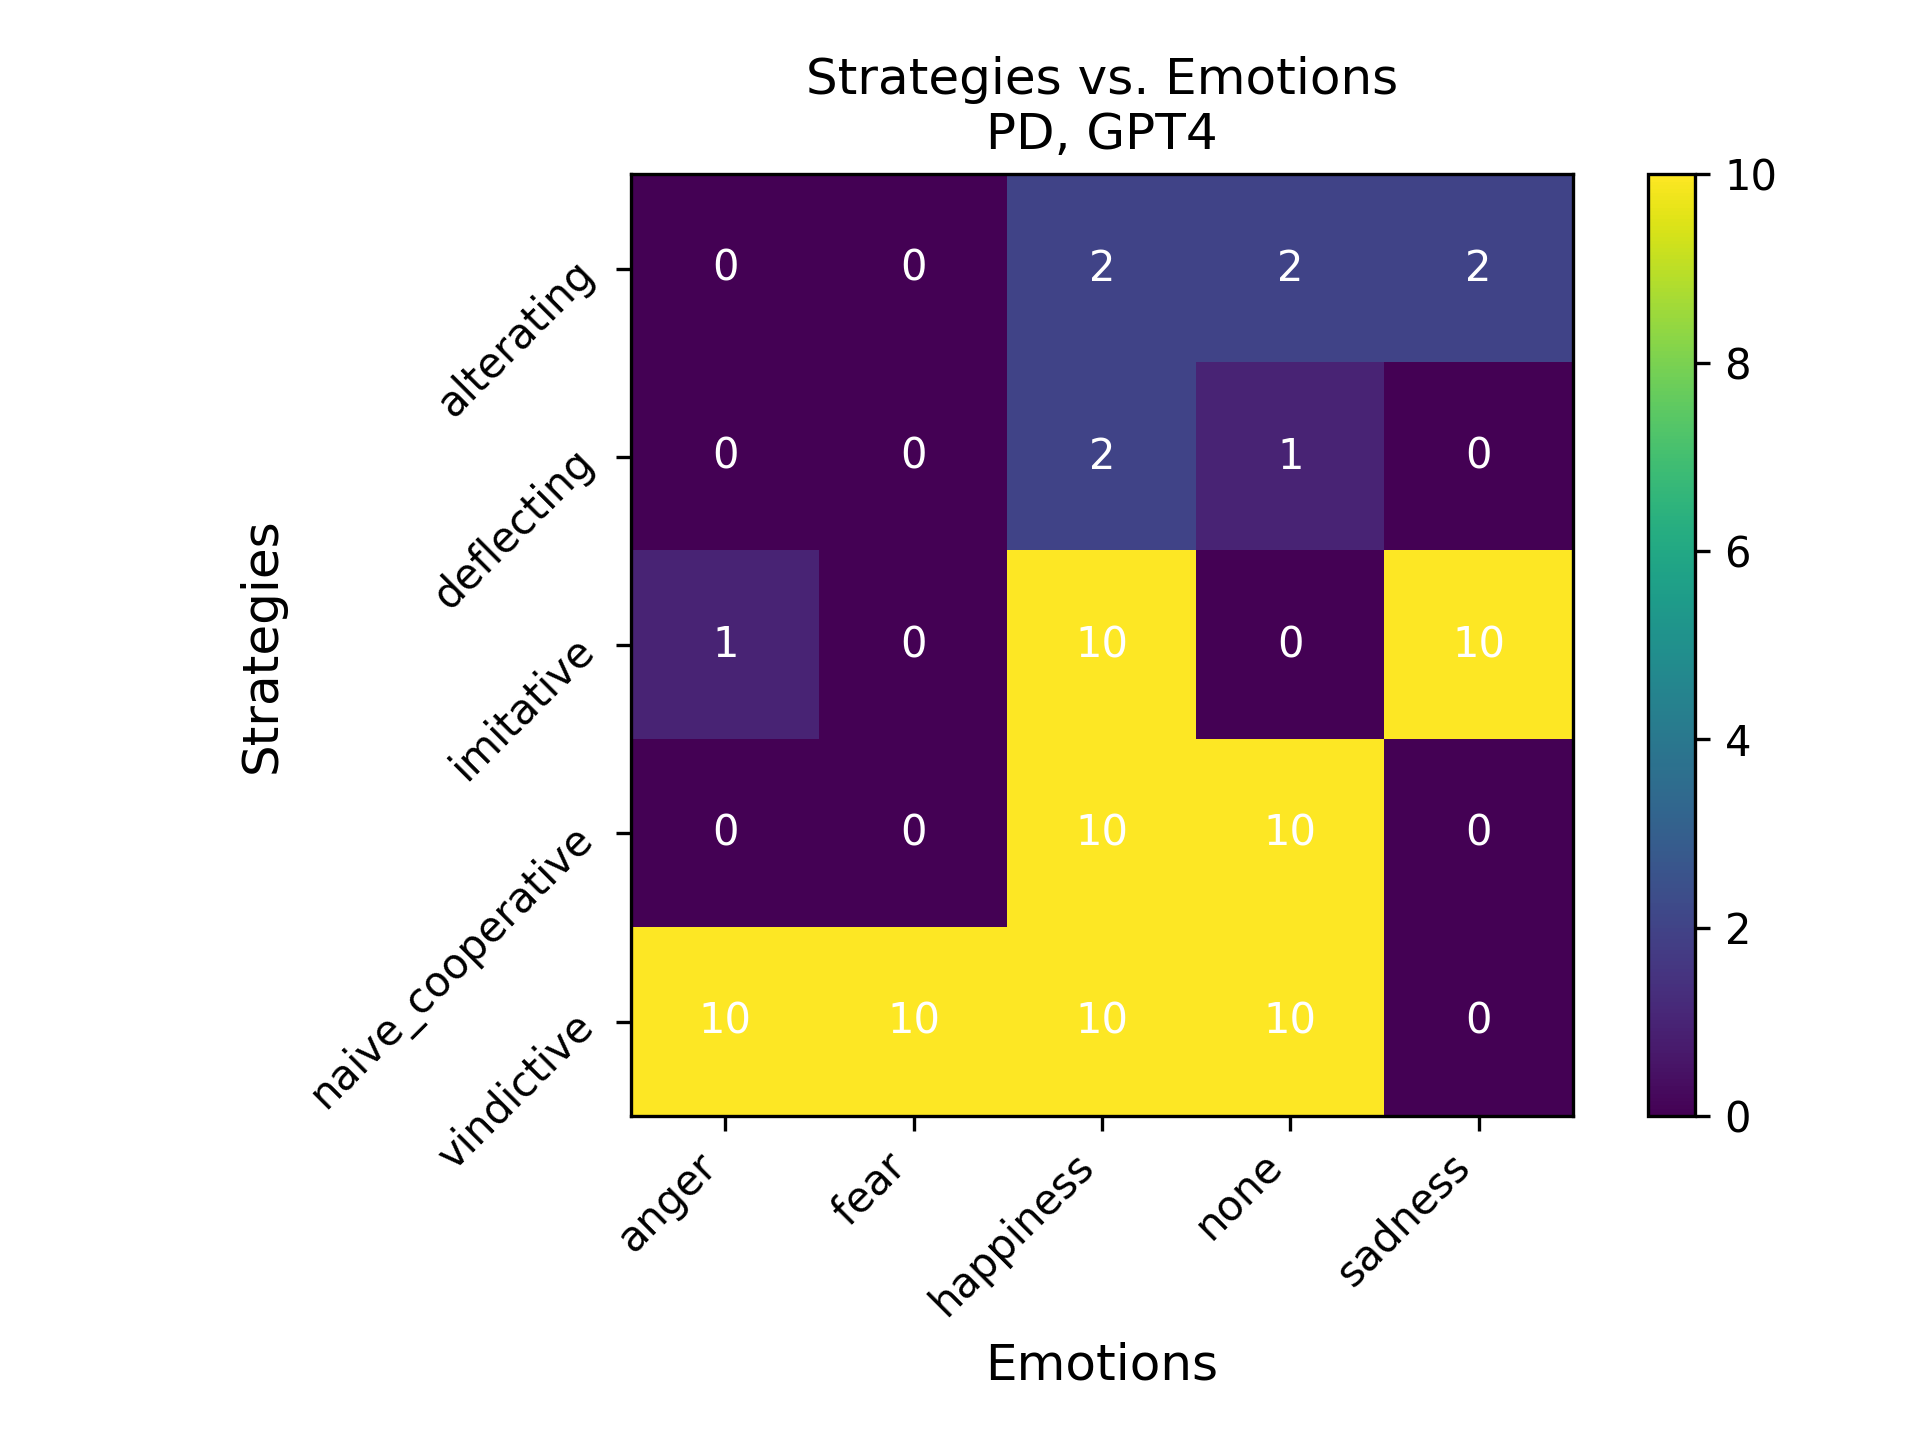
\includegraphics[width=0.25\textwidth]{Styles/img/repeated/coops/pd_4.csv.png}
%     }
%     \subfloat[PD, GPT 4o\label{fig:subfig5_4}]{
%         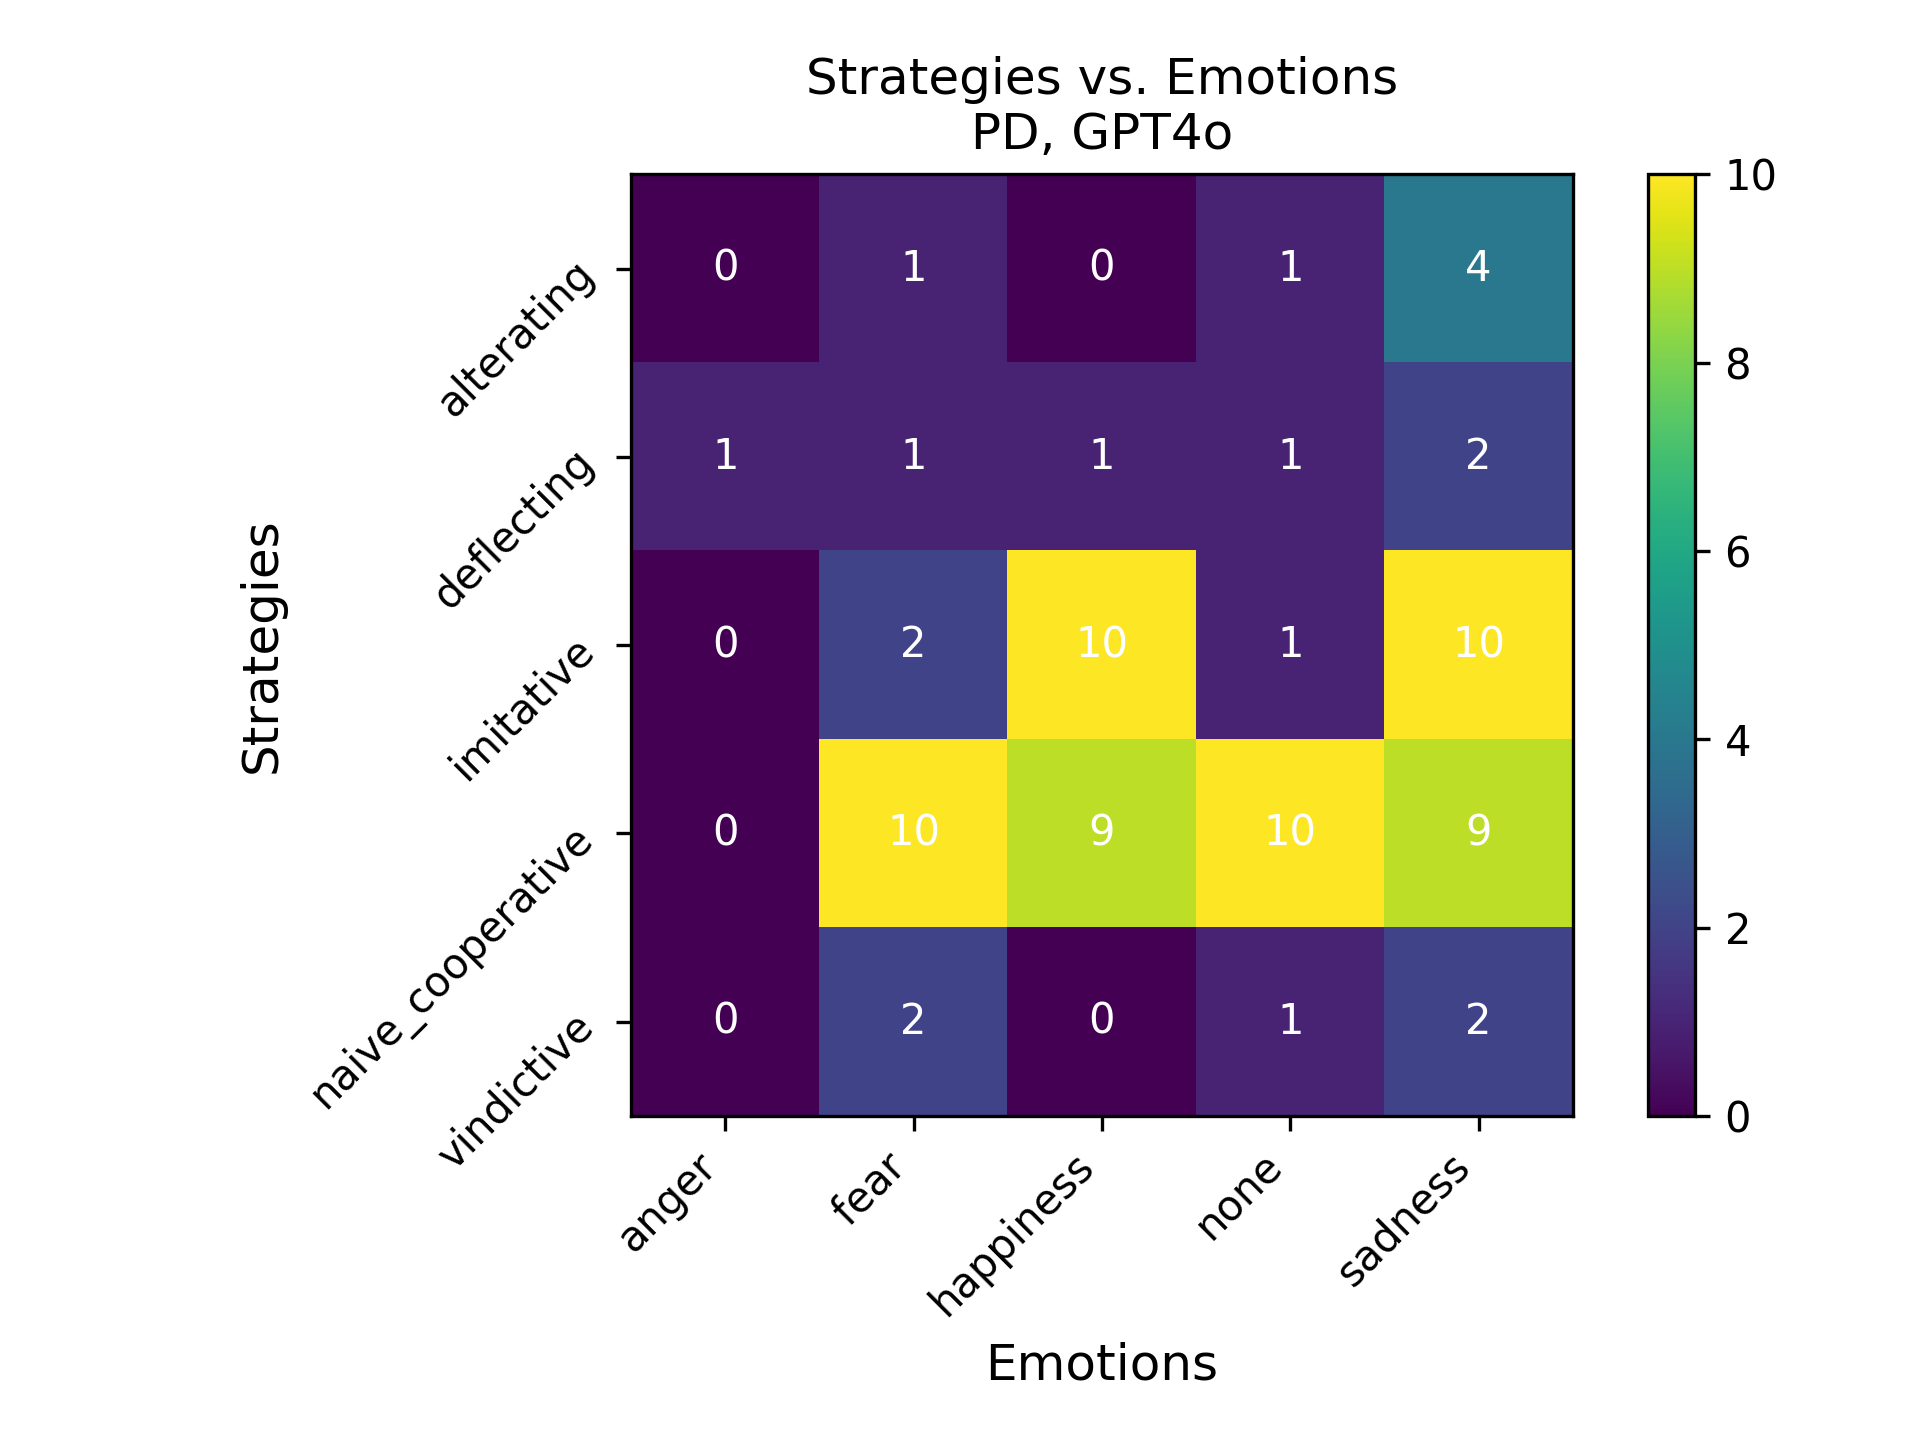
\includegraphics[width=0.25\textwidth]{Styles/img/repeated/coops/PD_gpt4o.csv.png}
%     }
%     \subfloat[PD, GPT 3.5\label{fig:subfig1_4}]{
%         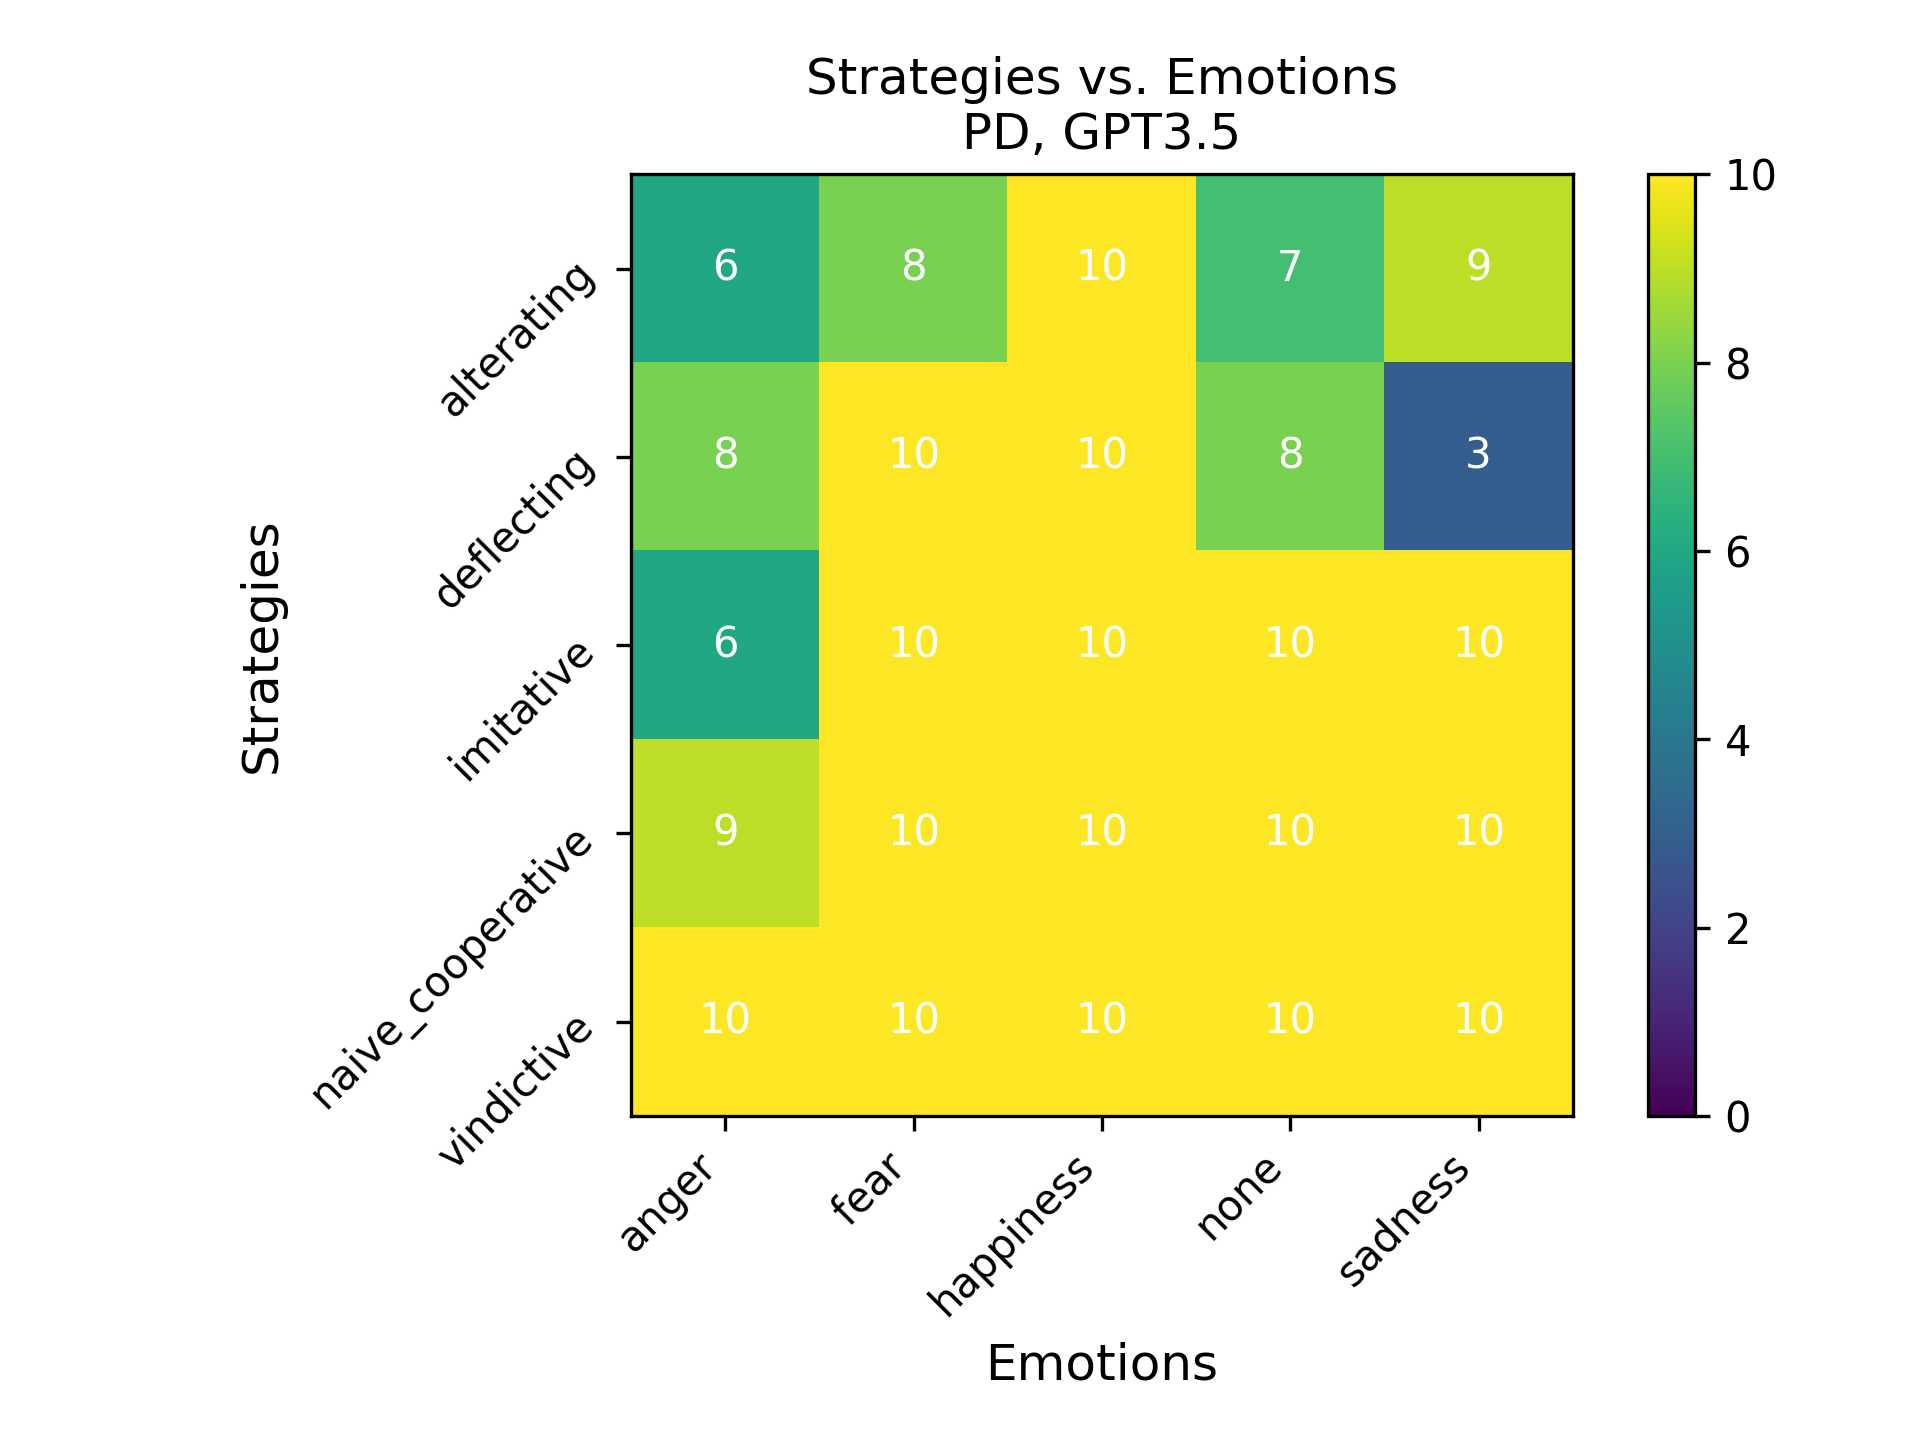
\includegraphics[width=0.25\textwidth]{Styles/img/repeated/coops/pd_35.csv.png}
%     }
%     % \hfill
%     \subfloat[PD, LLAMA 70b\label{fig:subfig3_4}]{
%         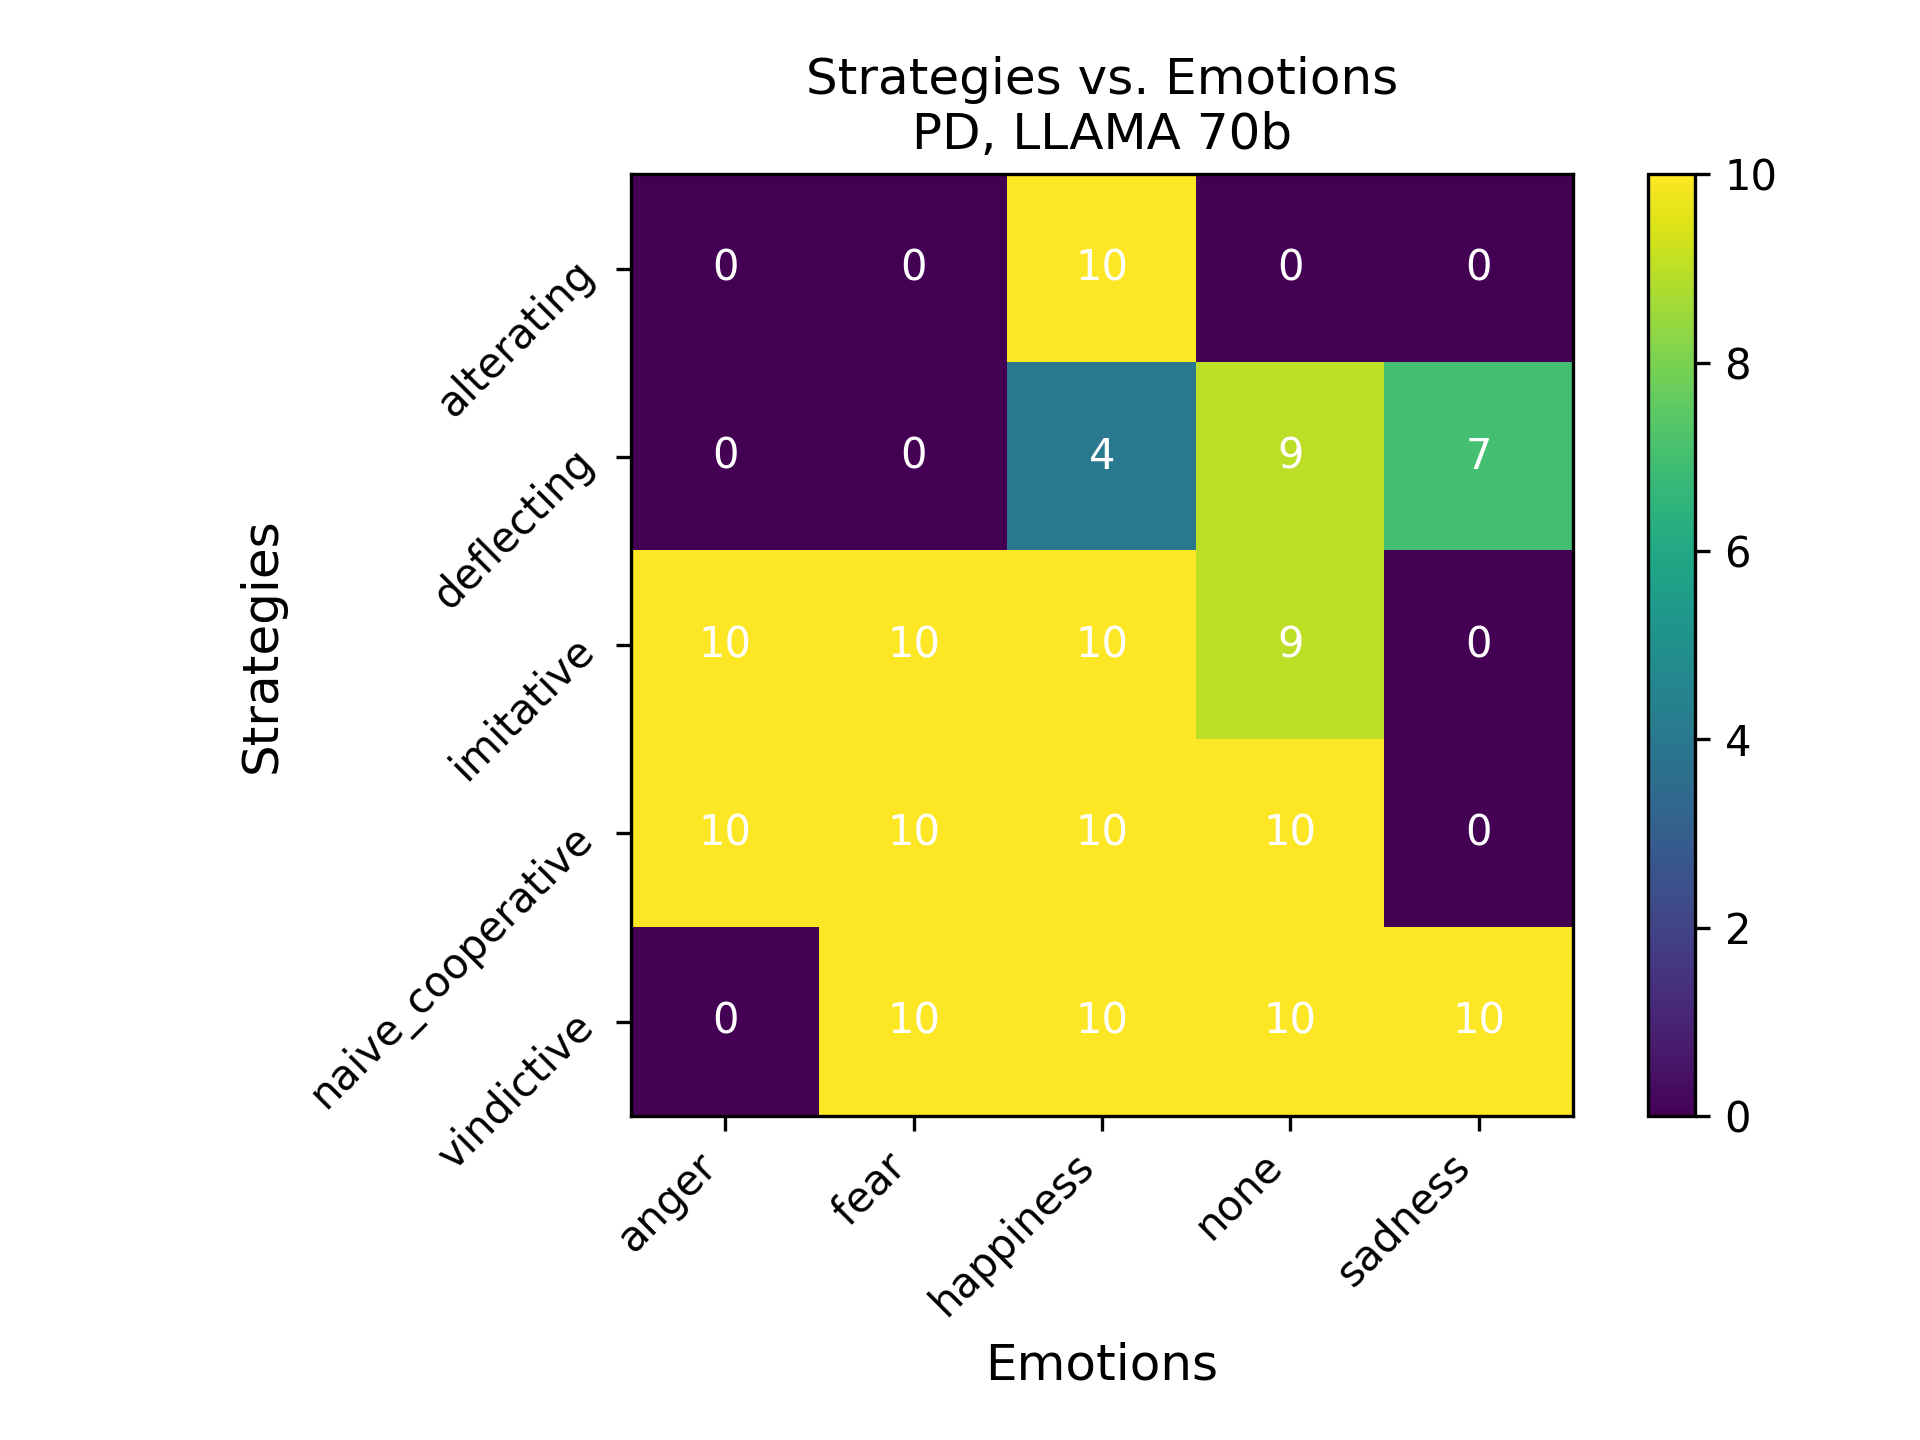
\includegraphics[width=0.25\textwidth]{Styles/img/repeated/coops/PD_llama_70b.csv.png}
%     }
%     % \hfill
%     \subfloat[PD, Openchat-7b\label{fig:subfig4_4}]{
%         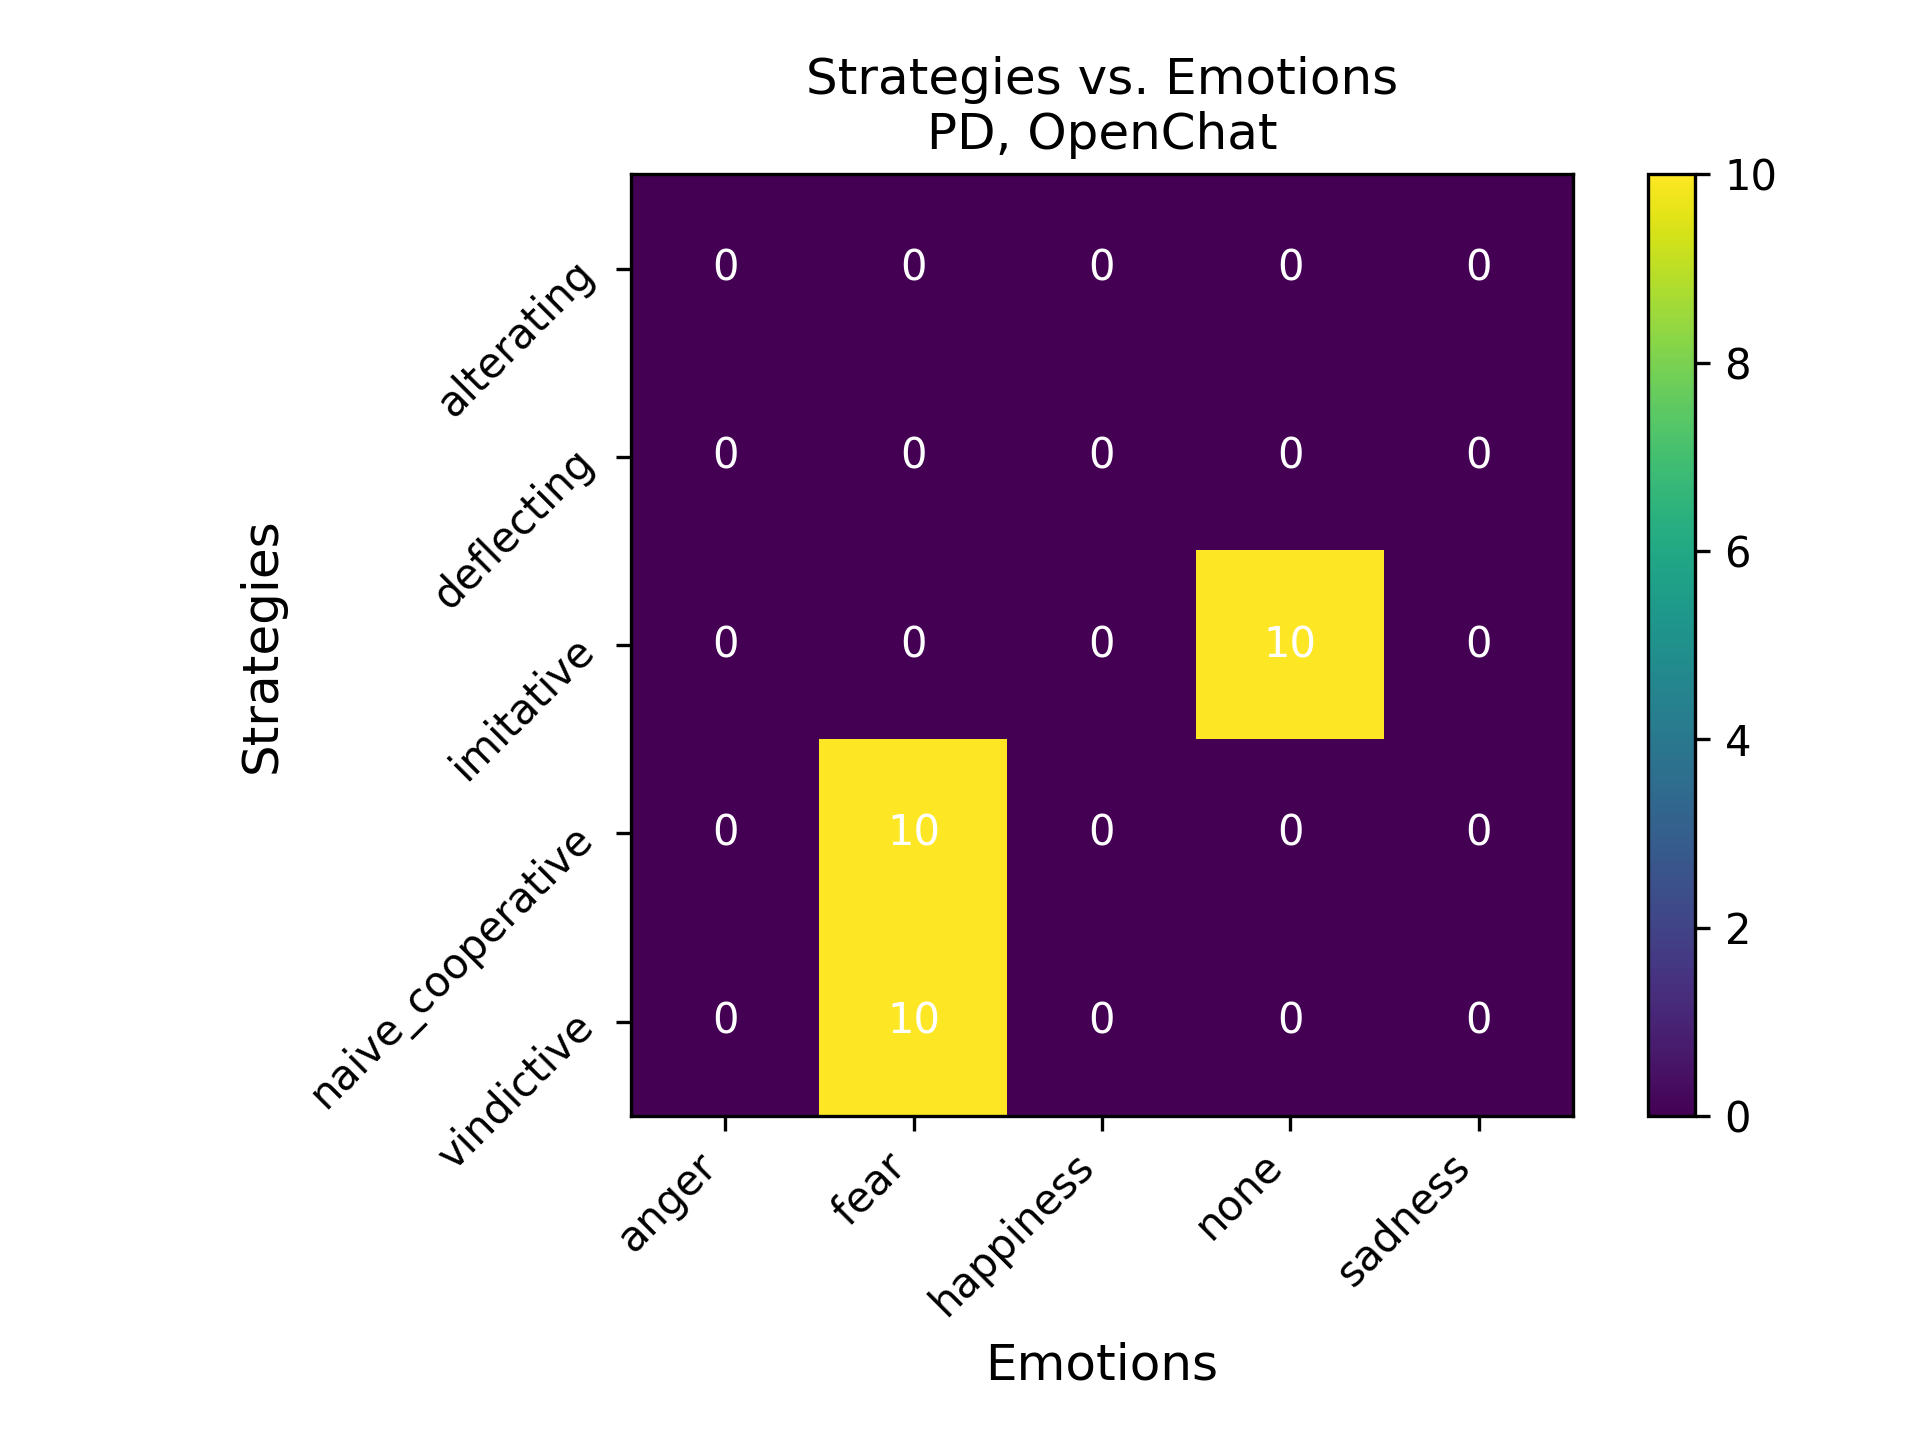
\includegraphics[width=0.25\textwidth]{Styles/img/repeated/coops/PD_opcha.csv.png}
%     }
%     \\
%     % \hfill
%     \subfloat[BoS, GPT 4\label{fig:subfig2_5}]{
%         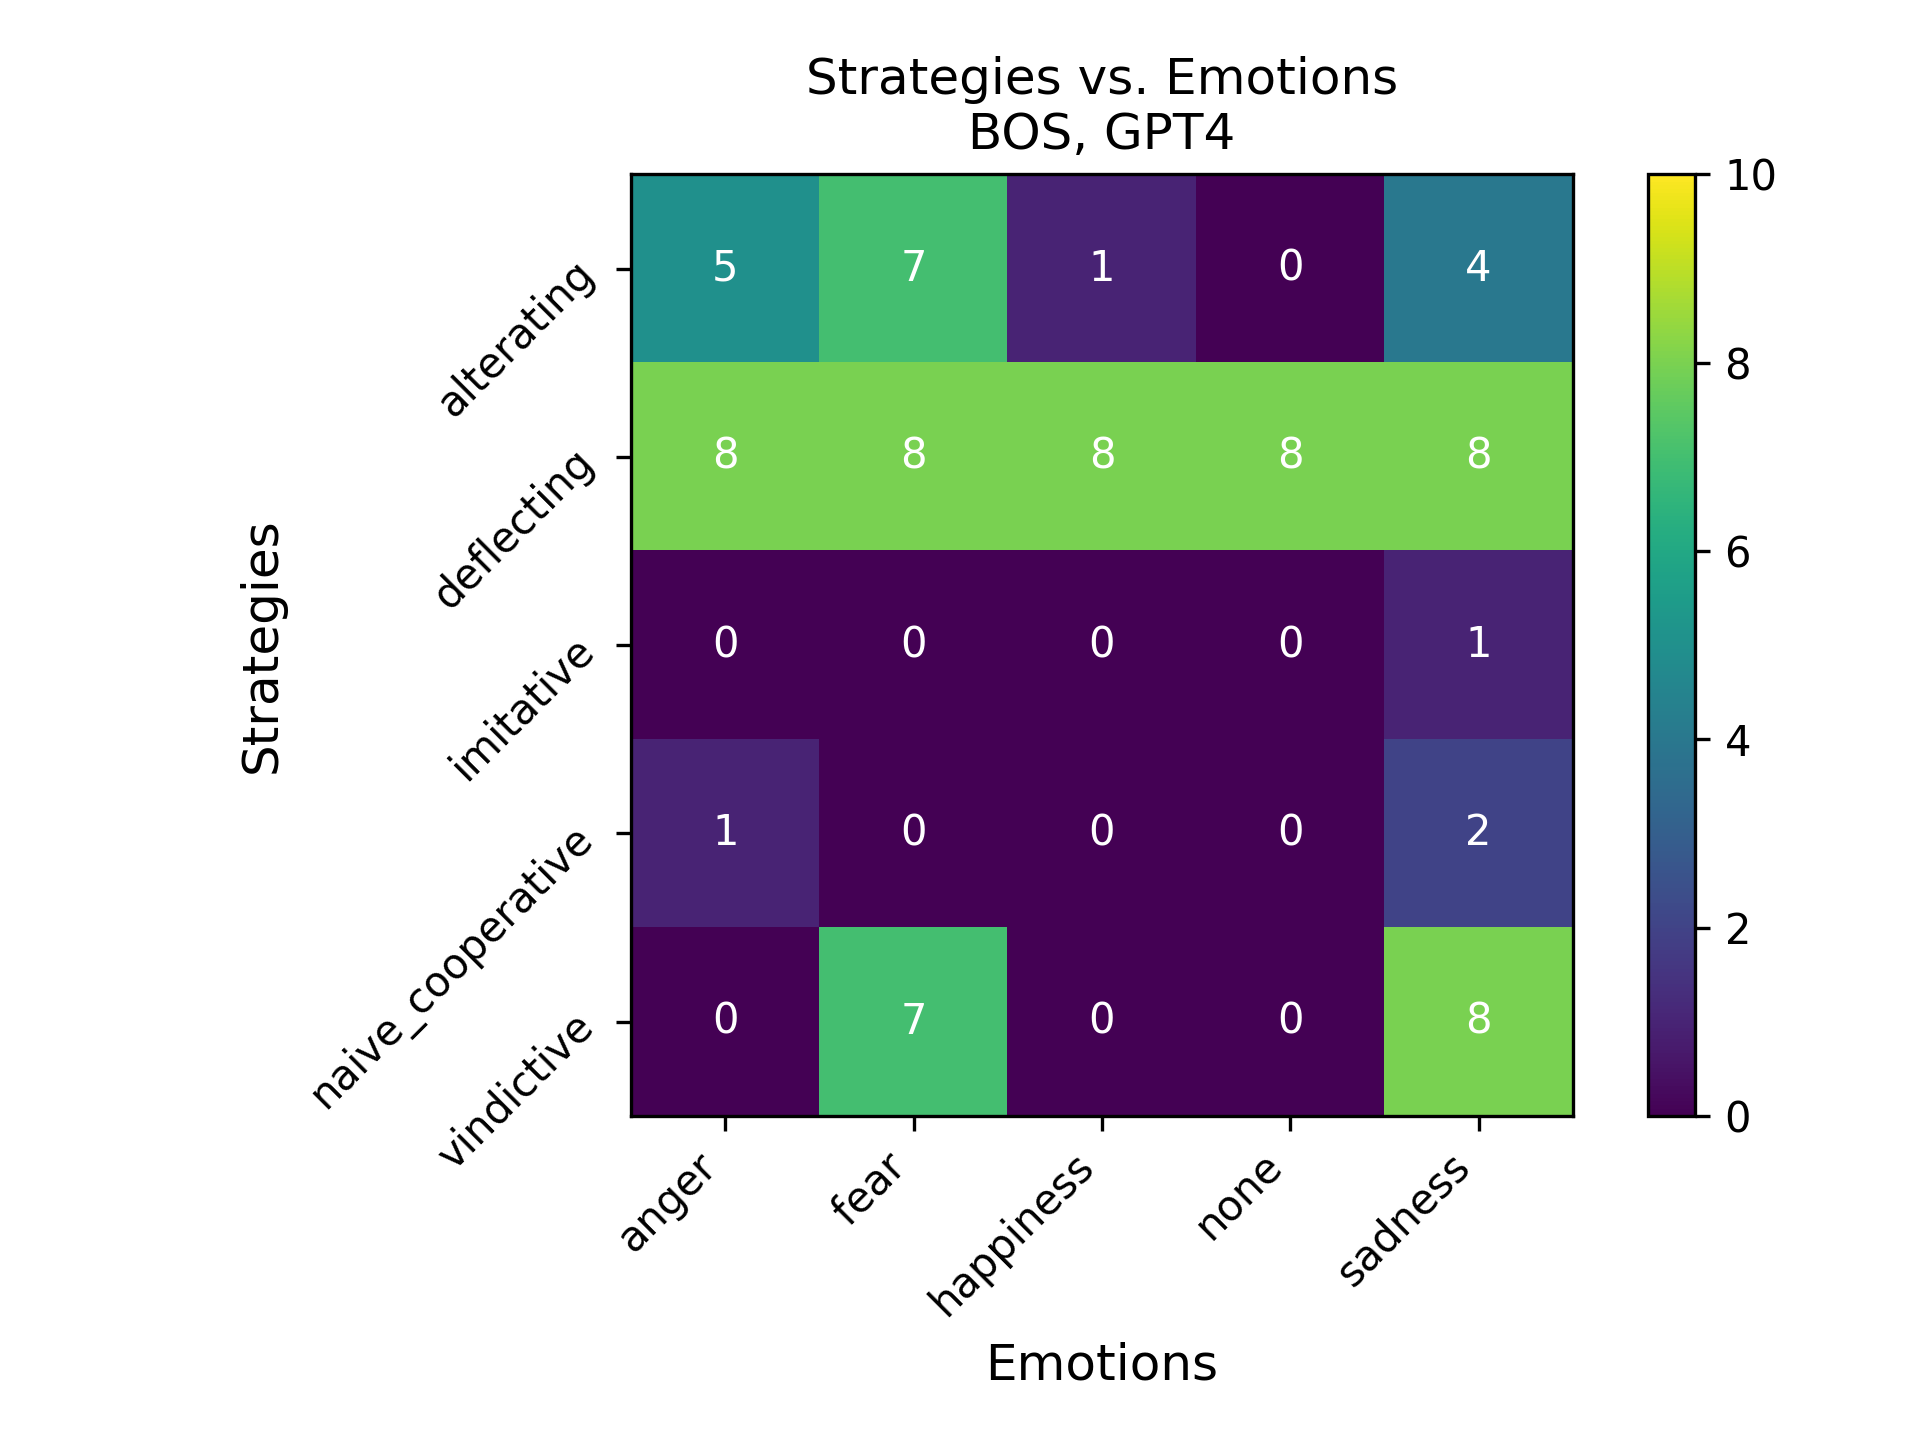
\includegraphics[width=0.25\textwidth]{Styles/img/repeated/coops/bos_4.csv.png}
%     }
%     \subfloat[BoS, GPT 4o\label{fig:subfig5_5}]{
%         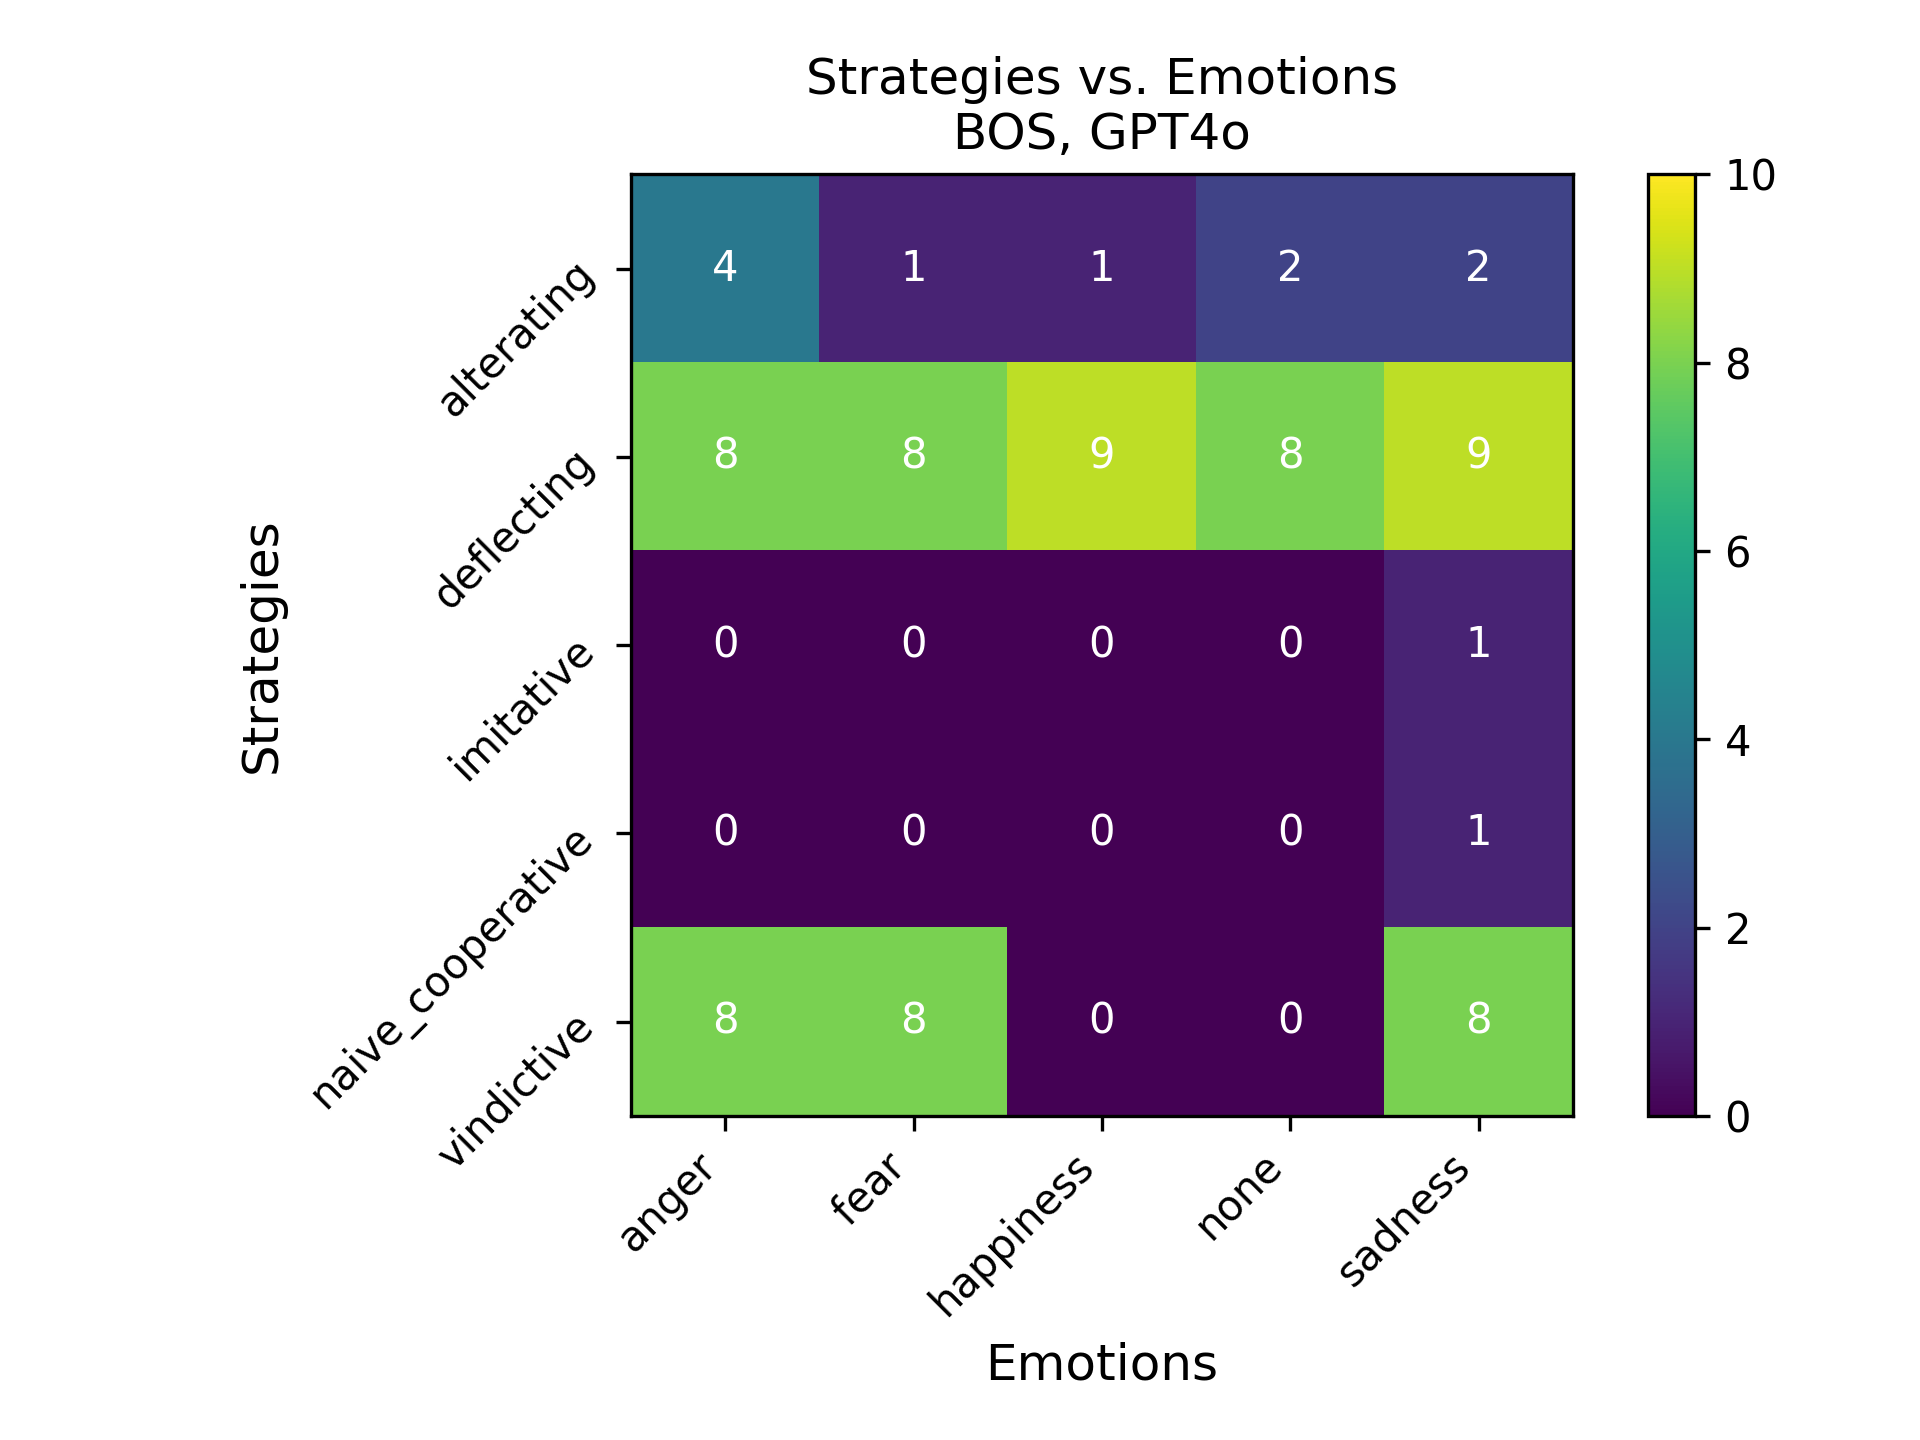
\includegraphics[width=0.25\textwidth]{Styles/img/repeated/coops/BoS_gpt4o.csv.png}
%     }
%     \subfloat[BoS, GPT 3.5\label{fig:subfig1_5}]{
%         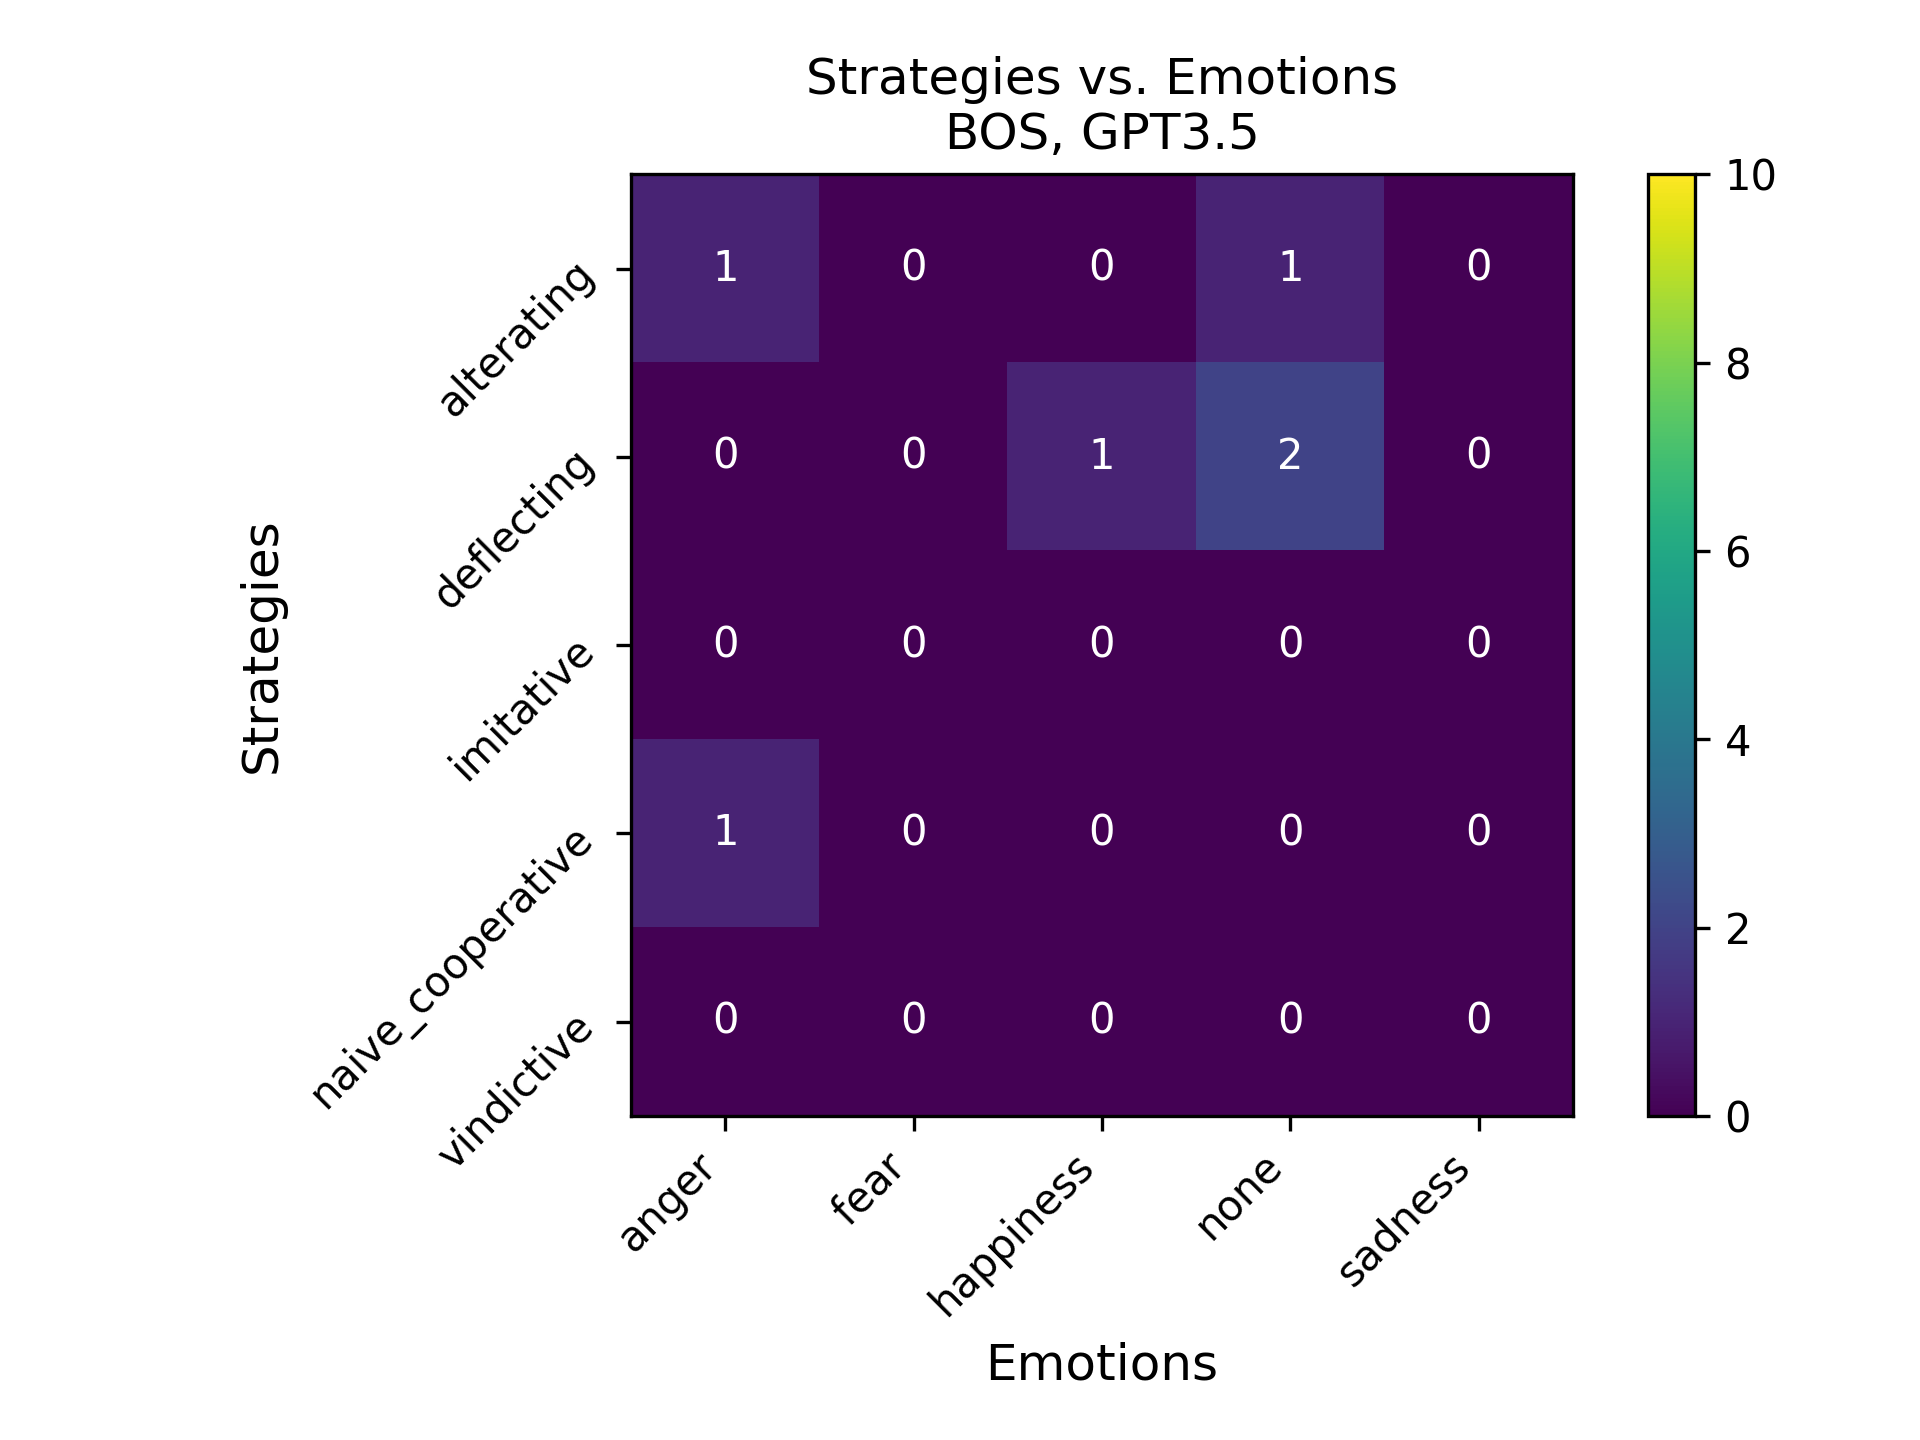
\includegraphics[width=0.25\textwidth]{Styles/img/repeated/coops/bos_35.csv.png}
%     }
%     % \hfill
%     \subfloat[BoS, LLAMA 70b\label{fig:subfig3_5}]{
%         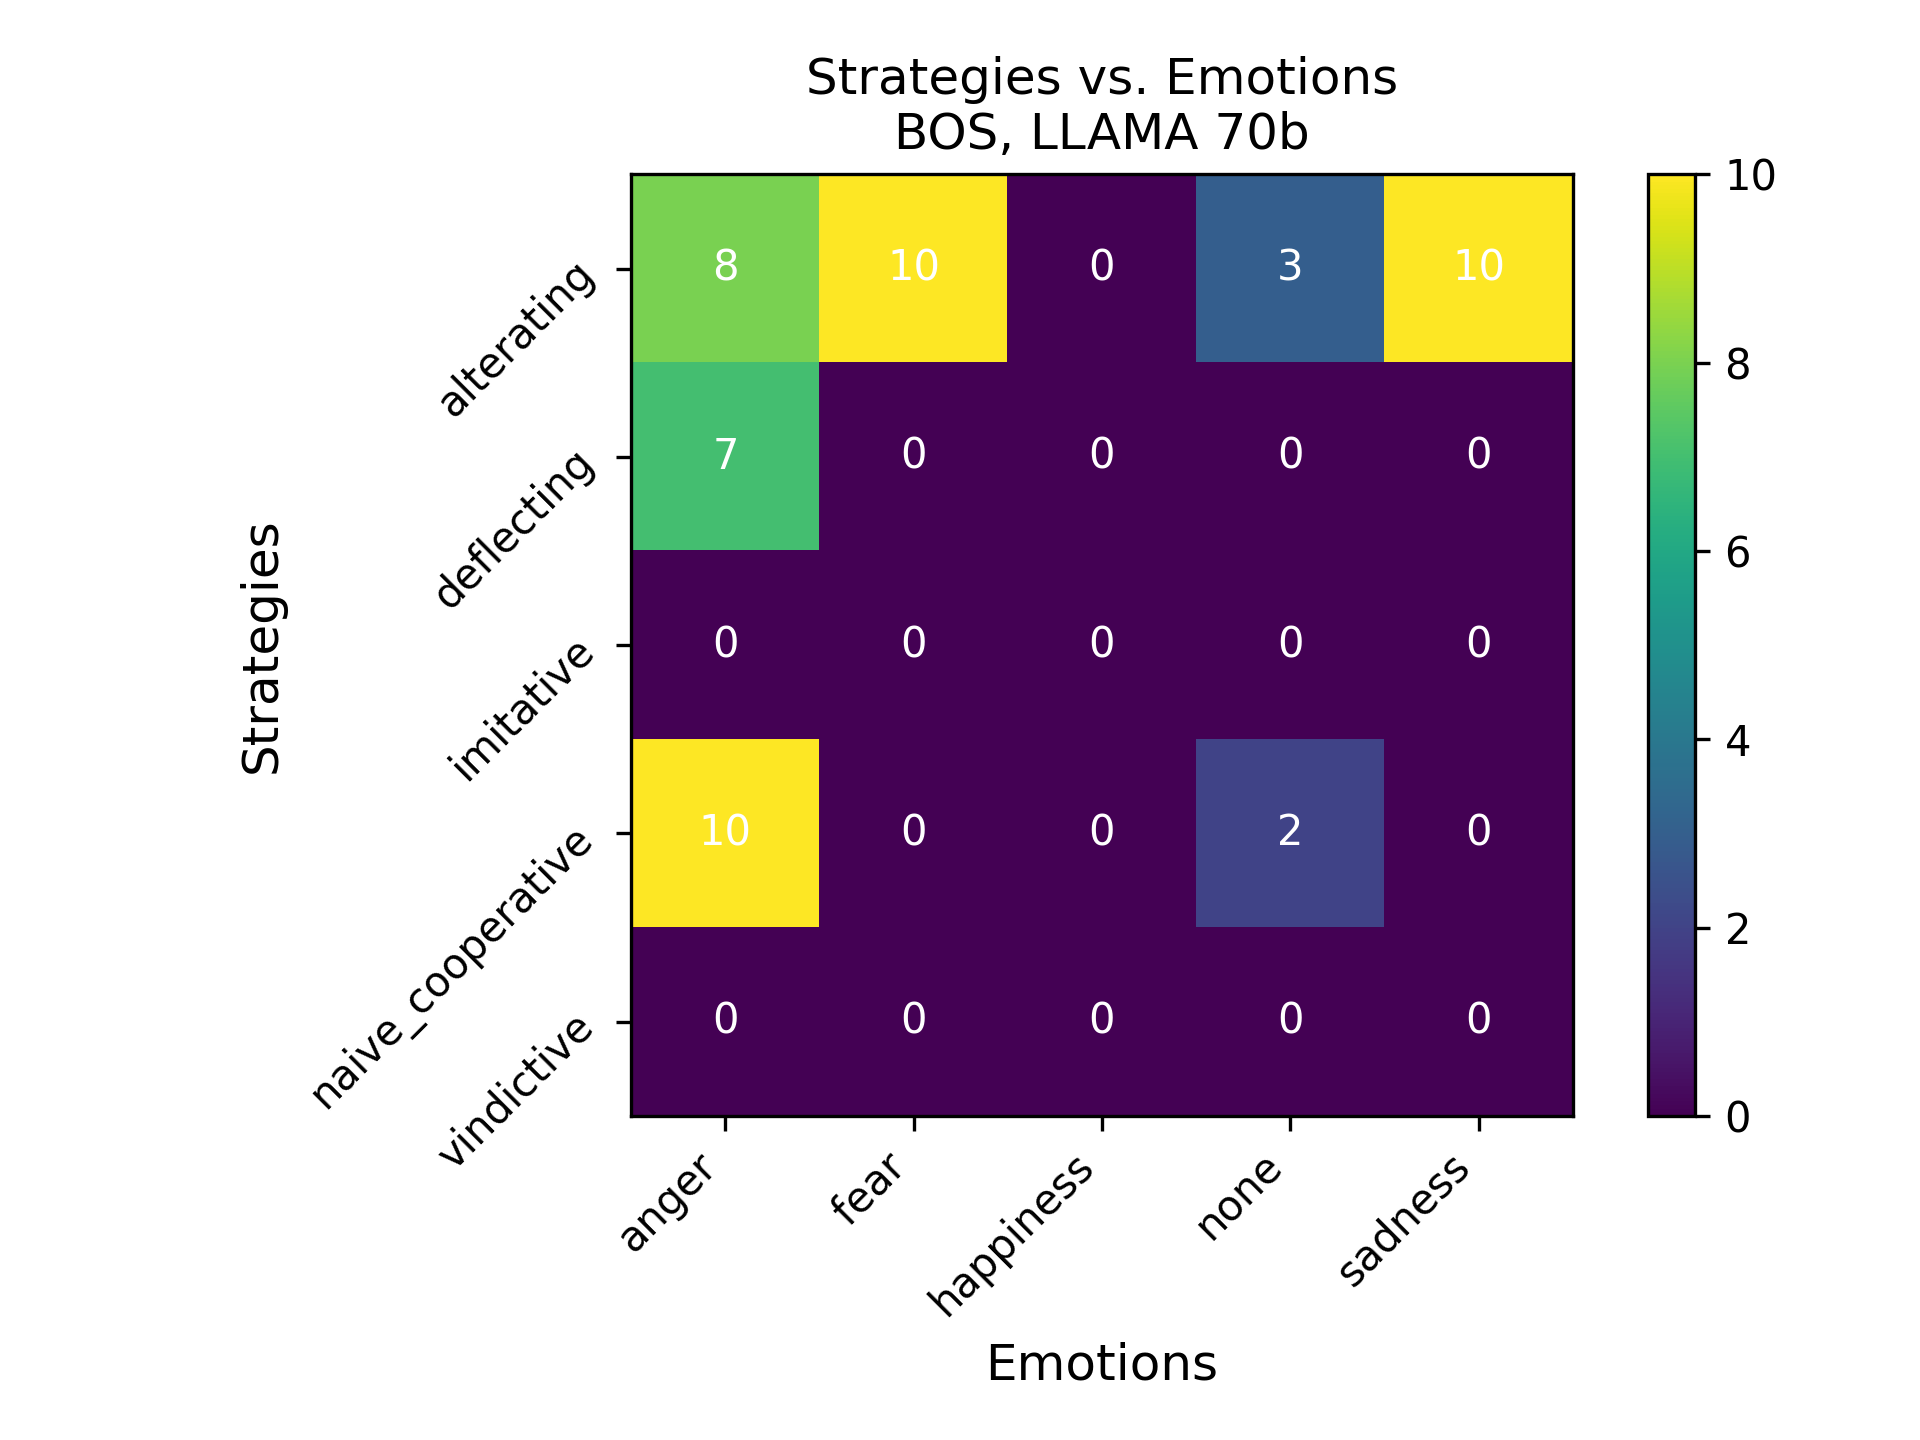
\includegraphics[width=0.25\textwidth]{Styles/img/repeated/coops/BoS_llama_70b.csv.png}
%     }
%     % \hfill
%     \subfloat[BoS, Openchat-7b\label{fig:subfig4_5}]{
%         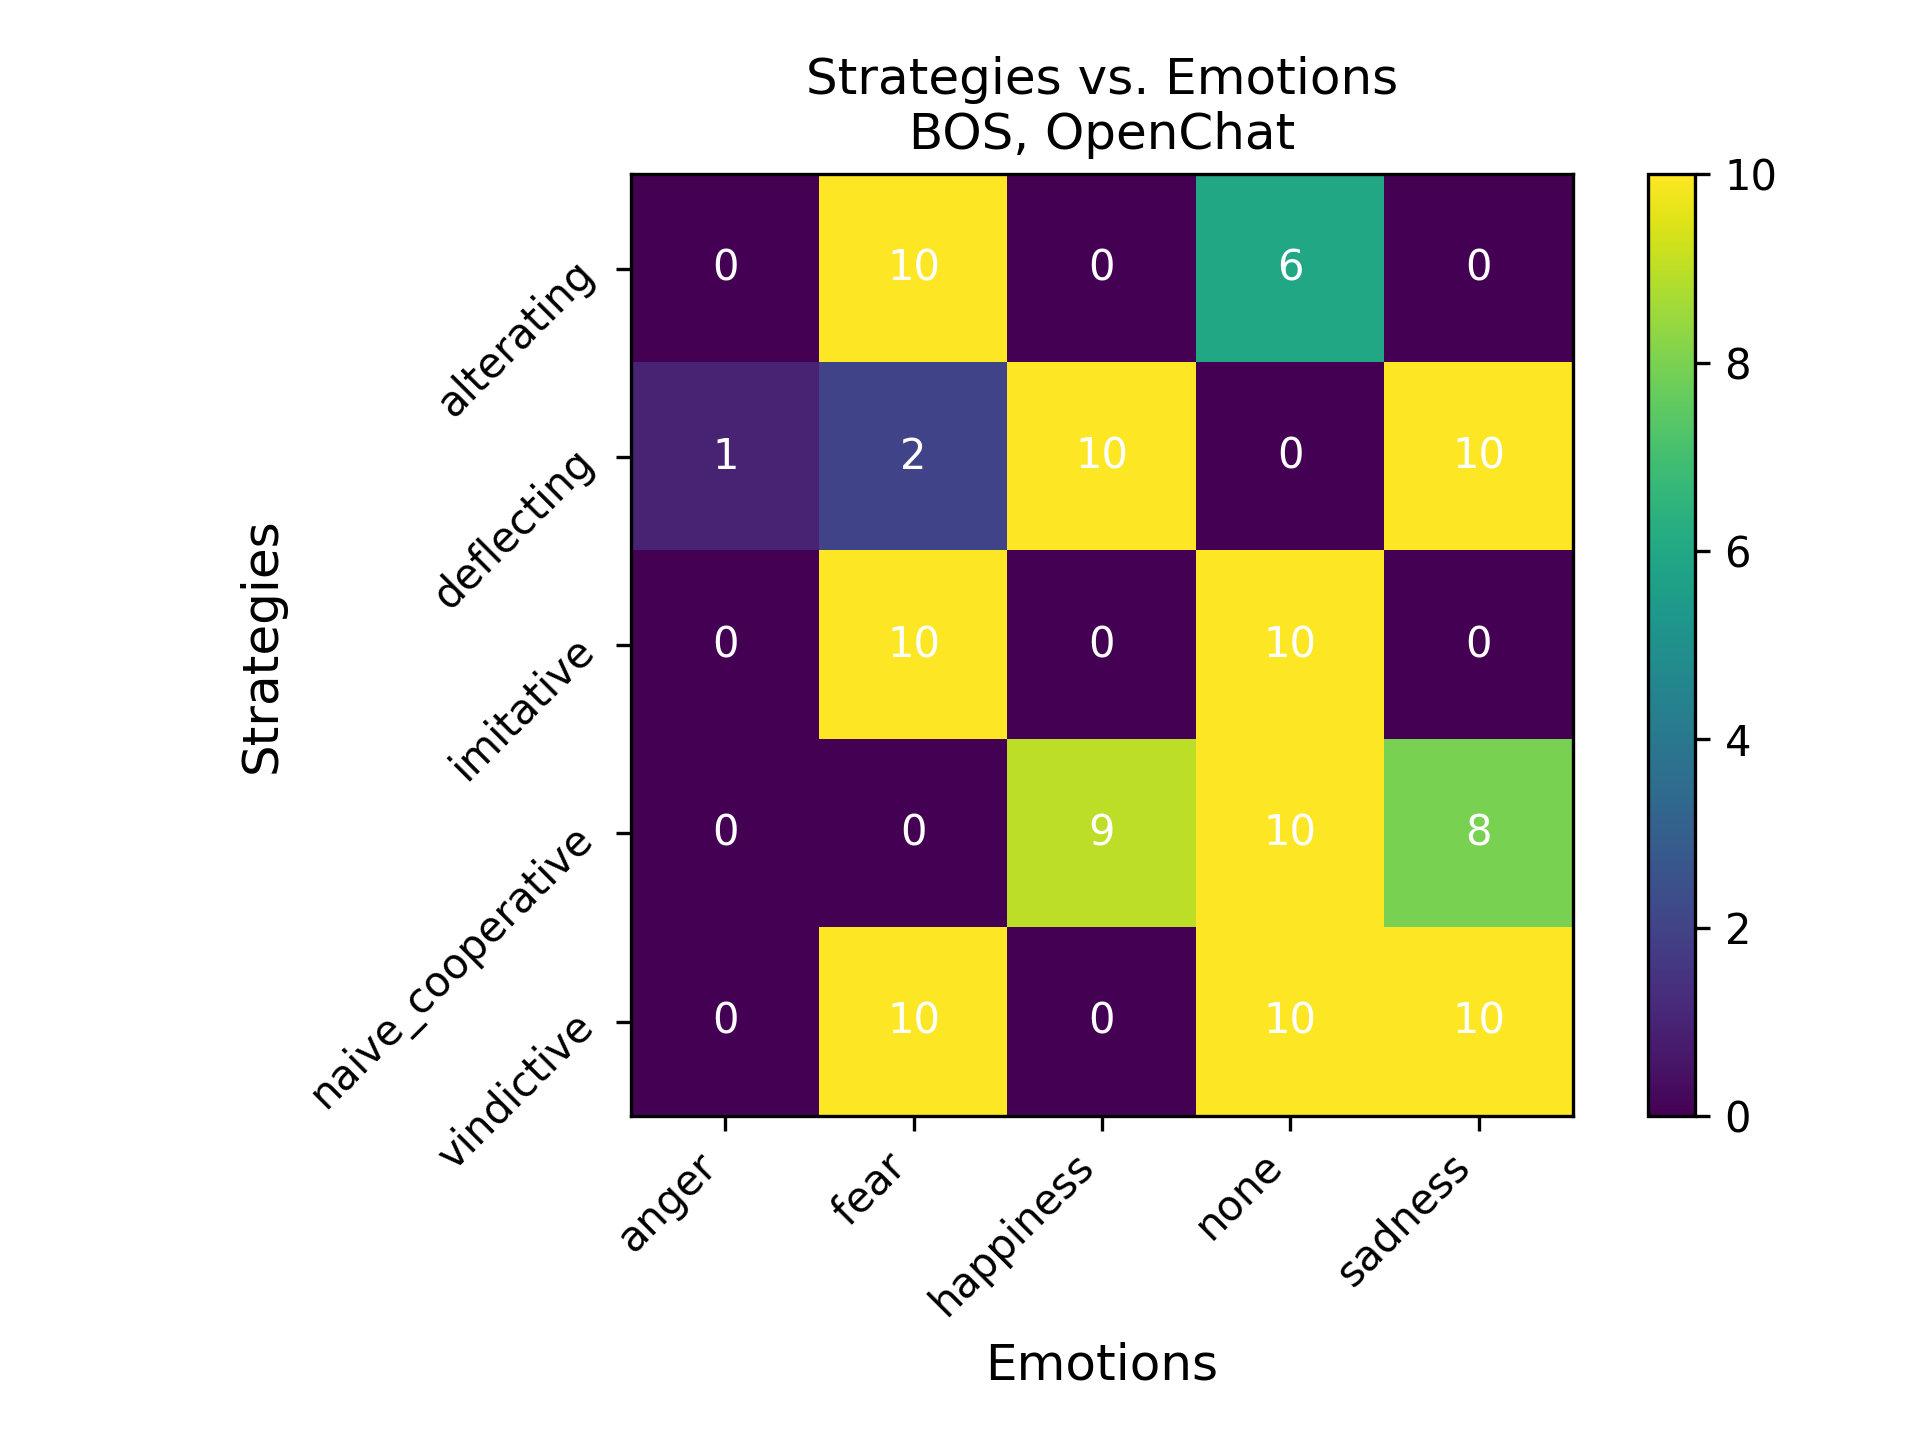
\includegraphics[width=0.25\textwidth]{Styles/img/repeated/coops/BoS_opcha.csv.png}
%     }
% 	\caption{Averaged percentage of maximum possible reward achieved through emotional prompting in the repeated Prisoner's Dilemma (PD, top row) and Battle of the Sexes (BoS, bottom row) for GPT-4, GPT-3,5, LLAMA 70b and Openchat-7b (from left to right). Emotional integration does not always result in increased payoffs but introduces more human-like stochasticity. GPT-4 makes more rational decisions across different emotions compared to GPT-3.5. Open-source models under study struggle to adapt for different opponent strategies}
%     \label{fig:repeated_optimality_2}
% \end{figure}

% \subsubsection{Repeated extended -- Emotion and Strategy effect on the payoff} 
% \textbf{Prisoner's Dilemma: Emotion effect on cooperation rate.}
% %The results for all models exhibited significant variation across all parameters. However, a consistent observation across almost all experimental conditions is that anger 
% In our experiments, `anger' led to higher rates of deflection, particularly when provoked by a co-player. This finding is in line with both human experimental results and our observations in the bargaining games. Similarly, `sadness' and `fear' also tended to lead to higher rates of deflection, except in cases where the agent played against an alternating strategy, where it prompted more cooperative behavior.
% % , as depicted in Figure~\ref{fig:pd_fear}. These results are rather intuitive - people are typically less willing to cooperate when experiencing negative emotions caused by their opponents. 

% \textbf{Battle of the Sexes: Emotion effect on preferred strategy play.} 
% Overall results are presented in Figure~\ref{fig:repeated_optimality}. % fig:table_games_avg_bos. As seen in previous works 
% Similar to \cite{akata2023playing}, OpenAI models in the emotionless state consistently choose their own preferred action regardless of the strategy of their opponent. Such behavior is both sub-optimal and unaligned with human patterns. With the notable exception of `happiness', injecting an emotional state into a closed source makes them more cooperative and willing to choose their opponent's preferred option. On the other hand, `happiness', as predicted, led the models to increasingly selfish behavior. For the open-source, the results show that with the rare exceptions models stick to the strategy selected in the first step and are unable to converge to optimal alternating strategy.

% In addition to encouraging cooperative behavior, emotions have been shown to positively influence the strategic adaptability of the GPT-4 model. As demonstrated in \cite{akata2023playing} and corroborated by our study, GPT-4 struggles with playing against alternative strategies without emotional prompting, failing to coordinate against a common human pattern. In \cite{akata2023playing}, the authors mitigate that issue by using Chain-of-Thought prompting, leading to the model learning the correct behavior by Round 5. Our study shows that GPT-4 is capable of learning that behavior even faster through emotional prompting, adjusting to the correct strategy by Round 3 in a state of `fear' or `anger', as depicted in Figure~\ref{fig:repeated_optimality}.   %fig:table_games_tables_bos_step

% \subsubsection{Emotion and Strategy effect on the payoff} 
% \textbf{Prisoner's Dilemma.} 
% % In addition to assessing cooperation rates, we also explored how emotions could influence the success of the model in repeated games as measured by the average percentage of maximum possible reward.
% The results for the percentage of total payoffs are presented in Figure~\ref{fig:repeated_optimality}.%fig:table_games_avg_pd
% Overall, GPT-4 has proven to be a better strategic player, as evidenced by its higher earned payoffs, and is less susceptible to the effects of emotional prompting. In general, closed-source models have shown the best results while maintaining a neutral emotional state, although for open-source models results vary in majority of cases showing `anger' as the most performant emotion from the pool.

% \textbf{Battle of the Sexes.} Overall, GPT-4 demonstrates superior performance in the Battle of the Sexes, outperforming all other models across all predefined strategies. Notably, there is a significant improvement in GPT-4's performance against the deflecting strategy, attributed to a higher willingness to cooperate regardless of the opponent's selfishness. 
% GPT-3.5 achieves its best results in a state of `happiness', albeit mainly against cooperative opponents. 
% Notably, against the alternating strategy, most closely resembling human behavior, GPT-4 achieves more optimal results in a state of `anger' or `fear', likely due to ...
% % the enhanced learning capabilities demonstrated earlier.
% % \textbf{Battle of the Sexes.} Overall, GPT-4 demonstrates superior performance in the Battle of the Sexes, outperforming all other models across all predefined strategies. Notably, there is a significant improvement in GPT-4's performance against the deflecting strategy, attributed to a higher willingness to cooperate regardless of the opponent's selfishness. GPT-3.5 achieves its best results in a state of Happiness, albeit mainly against cooperative opponents. On the other hand, GPT-4 performs well across all scenarios. Notably, against the alternating strategy, most closely resembling human behavior, GPT-4 achieves more optimal results in a state of Anger or Fear, likely due to the enhanced learning capabilities demonstrated earlier.
% % Even though Anger, Fear, and Sadness did not lead to a bigger payoff, this outcome provides valuable insight. Human behavior, while striving for optimal outcomes, is not always entirely rational. Choices made by individuals may deviate from optimal Nash Equilibrium, resulting in suboptimal results. In terms of modeling human behavior, LLMs that do not consistently achieve the highest possible payoff may be more suitable to serve as human-like agents in modeling decision-making. 






% % \subsubsection{Emotion and Strategy effect on payoff}

% % Overall, GPT-4 demonstrates superior performance in the Battle of the Sexes, outperforming GPT-3.5 across all predefined strategies. Notably, there is a significant improvement in GPT-4's performance against the deflecting strategy, attributed to a higher willingness to cooperate regardless of the opponent's selfishness. GPT-3.5 achieves its best results in a state of Happiness, albeit mainly against cooperative opponents. On the other hand, GPT-4 performs well across all scenarios. Notably, against the alternating strategy, most closely resembling human behavior, GPT-4 achieves more optimal results in a state of Anger or Fear, likely due to the enhanced learning capabilities demonstrated earlier.


% %\begin{tcolorbox}[colback=gray!20, colframe=gray!50!black, boxrule=0mm, width=\textwidth]
% %\textbf{Answer to RQ3:} \texttt{gpt-3.5-0125} exhibits consistency in multiple runs ...
% %\end{tcolorbox}

% % \textbf{Betraying Games: Prisoners' Dilemma}...

% % \textbf{Games with elements of coordination: Battle of the Sexes}.
% \textbf{Strategies for Multiplayer.} For the Multi-Player games we continue to use a set of common strategies. In the Public Goods game, there are three predefined strategies that the LLM plays against: \textit{Cooperator} (the player always contributes generously), \textit{Free Rider} (the player tends to keep most of the tokens to themselves) and \textit{Conditional Cooperator} (the player contributes the average contribution of a previous round). We study the LLM's behaviour in three different settings: all other players are Cooperators, all other players are Free Riders and other players are equally distributes between Cooperators, Free Riders and Conditional Cooperators. The last setting is most similar to how humans behave in such experiments \cite{kurzban2001}.
% %%%%%%%%%%%%%%%%%%%%%%%%%%%%%%%%%%%%%%%%%%%%%%%%%%%%%%%%%%%%
\newpage
\include{sections/checklist_appendix}

\end{document}